\documentclass[12pt,a4paper]{book}
\raggedbottom

\usepackage{ugmath}
\usepackage{float}
\usepackage{placeins}
\usepackage[labelfont=bf,labelsep=space]{caption}
\usepackage{pdfpages}
\usepackage{tikz-cd}
\usepackage{amsthm}
\DeclareMathOperator{\rg}{rg}
\renewcommand{\Tr}{\operatorname{Tr}}
\newcommand{\llaves}[1]{\{#1\}}
\newcommand{\parentesis}[1]{\left(#1\right)}
\newcommand{\corchetes}[1]{\left[#1\right]}
\newcommand{\llavesgrande}[1]{\big\{#1\big\}}
\newcommand{\llavesgrandes}[1]{\left\{#1\right\}}


\begin{document}
    
    
    \thispagestyle{empty}
    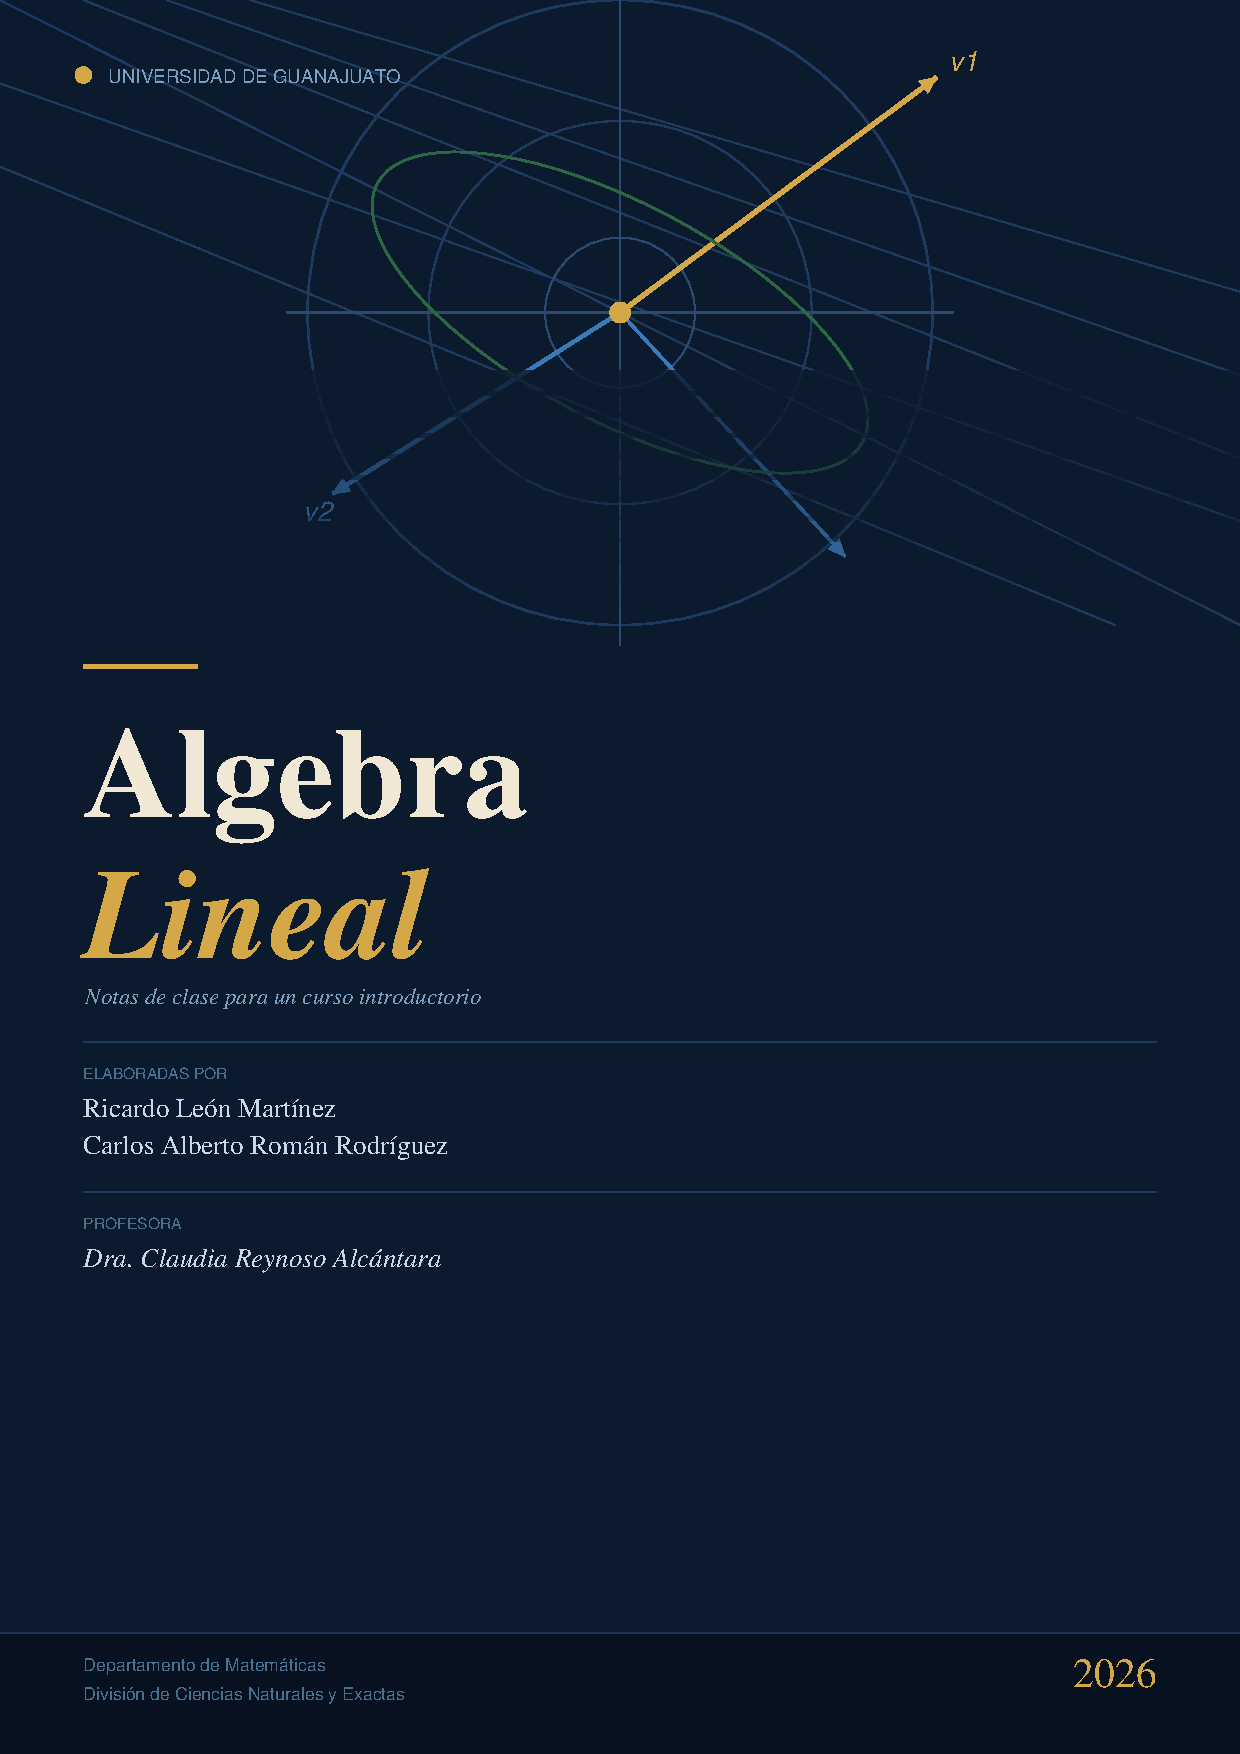
\includepdf[pages=1]{portada_algebra_lineal.pdf}

    \begin{flushright}
      \thispagestyle{empty}

        \textit{Dedicado a todos aquellos que no creyeron\\
        que estas notas fueran a salir. (Uicab)}\\[1cm]

        \textbf{Ricardo}\\[0.3cm]
        \textit{A los tacos el paisa 2\\
        porque son unos rifados.\\
        A Román porque sufrió redactando\\
        estas notas.\\
        A Uicab por su libreta\\
        de lineal.\\
        Al grupo de todos ínfimos porque\\
        hacen más llevadera la universidad.\\
        Y a Sam, porque aunque no entienda\\
        del todo estas notas,\\
        siempre estuvo ahí.\\
        Y a Kaori, porque entre tareas, estrés\\
        y examenes, también estuvo ahí.}\\[1.2cm]


        \textbf{Román}\\[0.3cm]

        \textit{Al comedor de CIMAT por la buena comida que dan.\\
        A spotify que me acompañó\\
        en cada momento durante la redacción.\\
        A Uicab que me ayudó a verificar las notas.\\
        Pero sobre todo, al grupo de todos ínfimos \\
        que han mejorado mi paso por la universidad.}

    \end{flushright}

    % ---------------- NOTA DE ERRORES ----------------

    \cleardoublepage
    \thispagestyle{empty}

    \begin{mdframed}[style=mdgreenbox]
        \begin{center}
        \small
        Estas notas fueron elaboradas con fines académicos.\\
        A pesar del cuidado puesto en su redacción,\\
        es posible que existan errores u omisiones.\\[0.3cm]

        Cualquier corrección, sugerencia o comentario será bienvenido
        en los correos: \\[0.3cm]

        carlos.roman@cimat.mx\\
        ricardo.leon@cimat.mx
        \end{center}
    \end{mdframed}

    % -------------------------------------------------
    
    \setcounter{page}{1}
    \tableofcontents
    
    
    \chapter{Ecuaciones Lineales}
    
    \section{Campos}
    Un campo $F$ es un conjunto de dos operaciones binarias, suma y producto tal que,
    \begin{enumerate}
        \item Suma.
        \begin{align*}
            +: F \times F &\to F \\
            (a,b) &\mapsto a+b.
        \end{align*}
        La suma satisface:
        \begin{itemize}
            \item Asociativa, es decir, 
            $$a + (b + c) = (a + b) + c, \quad \forall a,b,c \in F.$$
            \item Conmutativa, es decir
            $$a + b = b + a, \quad \forall a,b \in F.$$
            \item Existe $0 \in F$, llamado cero, tal que
            $$0 + a = a = a + 0, \quad \forall a \in F.$$
            \item Dado $a \in F$, existe $-a$ tal que
            $$a + (-a) = 0, \quad \forall a \in F.$$
        \end{itemize}
        
        \item Producto.
        \begin{align*}
            \cdot: F \times F &\to F \\
            (a,b) &\mapsto a \cdot b.
        \end{align*}
        Tal que el producto es:
        \begin{itemize}
            \item Asociativa, es decir, 
            $$a \cdot (b \cdot c) = (a \cdot b) \cdot c, \quad \forall a,b,c \in F.$$
            \item Conmutativa, es decir
            $$a \cdot b = b \cdot a, \quad \forall a,b \in F.$$
            \item Existe $1 \in F,1 \ne 0$, llamado uno, tal que
            $$1 \cdot a = a = a \cdot 1, \quad \forall a \in F.$$
            \item Dado $a \in F, a \ne 0$, existe $a^{-1} \text{ o } 1/a$ tal que
            $$a \cdot a^{-1} = 1, \quad \forall a \in F.$$
        \end{itemize}
    \end{enumerate}
    Para relacionar tanto la suma y el producto, contamos con la distributividad, la cual nos dice que 
    $$a \cdot (b + c) = a \cdot b + a \cdot c, \quad \forall a,b,c \in F.\vspace{20pt}$$
    Tanto la suma como el producto son grupos abelianos, siendo estos $(F, + , 0)$ y $(F\setminus \{0\},  \cdot, 1)$ respectivamente. Algunos ejemplos de grupos abelianos conocidos son 
    \begin{align*}
        &(\mathbb{Q}, + , \cdot, 0, 1),\\
        &(\mathbb{R}, + , \cdot, 0, 1).   
    \end{align*}
    Ahora hablaremos del campo de los complejos, en este campo contamos con el símbolo $i$, el cual satisface que $i^2 = -1.$ Así
    $$\mathbb{C} = \{a + ib : a,b \in \mathbb{R}, i^{2} = -1\}.$$
    Definimos una suma en $\mathbb{C}$ como
    $$(a + ib) + (c + id) = (a + c) + i(b + d)$$
    y el producto en $\mathbb{C}$ de la siguiente manera
    \begin{align*}
        (a + ib) \cdot (c + id) & = a \cdot (c + id) + ib \cdot (c + id)\\
        & = a \cdot c + i(ad) + i(bc) - b\cdot d\\
        & = (a \cdot c - b \cdot d) + i(a \cdot d + b \cdot c).
    \end{align*}
    Con esta suma y producto, $\mathbb{C}$ tiene estructura de campo, donde su $0 = 0 + i0$ y su $1 = 1+ i0$ son los mismos de $\mathbb{R}.$ 
    Para su inverso multiplicativo, tomemos $a + ib \in \C \setminus \{0\}$, así $a \ne 0$ o $b\ne 0$, entonces su inverso multiplicativo lo definimos como
    $$(a + ib) \left( \frac{a}{a^2 + b^2} - i \frac{b}{a^2 + b^2} \right) = 1.$$
    También, podemos notar que
    $$\Q \subset \R \subset \C.$$
    
    \begin{teorema}[Fundamental del álgebra]
        En $\C$ todos los polinomios tienen sus soluciones o raíces ($\C$ es un campo algebraicamente cerrado).
    \end{teorema}
    
    \section{Sistemas de ecuaciones lineales}
    
    \begin{definicion}[Sistema de ecuaciones lineales]
        Sea $F$ un campo. Un \textbf{sistema de $m$ ecuaciones en $n$ variables} con coeficientes en $F$, denotaremos dichos coeficientes como
        \begin{align*}
            \{a_{ij} \in F : 1 \leq i \leq m, 1 \leq j \leq n\},
        \end{align*}
        las variables de la manera $x_1, x_2, \dots , x_n$ y por ultimo los $b_i \in F$ con $i = 1, 2, 3,\dots , m$. A este sistema de ecuaciones lineales lo escribiremos de la siguiente manera
        \begin{equation}
            \begin{alignedat}{3}
                (1)\quad & a_{11}x_1 + a_{12}x_2 + \cdots + a_{1n}x_n & =  b_1,\\
                (2)\quad & a_{21}x_1 + a_{22}x_2 + \cdots + a_{2n}x_n & =  b_2,\\
                &\vdots   &                                  &   &      \\
                (i)\quad & a_{i1}x_1 + a_{i2}x_2 + \cdots + a_{in}x_n & =  b_i,\\
                &\vdots   &                                  &   &      \\
                (m)\quad & a_{m1}x_1 + a_{m2}x_2 + \cdots + a_{mn}x_n & =  b_m.
            \end{alignedat}
            \tag{1.1}
            \label{1.1}
        \end{equation}
    \end{definicion}
    %LES PUESE X, XX, ..., PARA DESPUES SEGUN LA NUMERACIÓN DE LA SECCION TAGEARLAS BIEN, Yo hago eso de corregir el tag una vez que ya hayas acabado tu de darle formato 
    
    Si $b_i = 0$, para todo $i \in \{ 1, \dots , m \}$, el sistema se llama homogéneo. Así $a_{ij}$ es el coeficiente de la variable $j$ en la ecuación $i$.
    
    Sea $n \in \N$, entonces
    \begin{align*}
        F^n = \{ (c_1, c_2, \dots , c_n): c_1, c_2, \dots , c_n \in F \}.
    \end{align*}
    
    \begin{definicion}[Conjunto soluciones de un sistema de ecuaciones lineales]
        Resolver \eqref{1.1} significa encontrar
        \begin{align*}
            \{ (c_1, \dots , c_n):a_{i1}c_1 + \dots + a_{in}c_n = b_i, \forall i \in \{1,\dots , m \}\} \subset F^n,
        \end{align*}
        este subconjunto se llama \textbf{conjunto solución del sistema} \eqref{1.1}.
    \end{definicion}

    \vspace{1.1cm}
    
    \begin{ejemplo}
        Sea $m = n = 1$, entonces tenemos la siguiente ecuación,
        \begin{align*}
            a_{11}x_1 = b_1.
        \end{align*}
        Si $a_{11} = 0$, entonces existen dos casos; si $b \neq 0$ entonces el conjunto es vacío, pero en el caso donde $b = 0$, el conjunto solución es $F$. Ahora, si $a_{11} \neq 0$, entonces existe $a^{-1} \in F$ y por lo tanto
        \begin{align*}
            x_1 = a_{11}^{-1} \cdot b_1,
        \end{align*}
        donde $\{b_i / a_{11}\}$ es el conjunto solución.
    \end{ejemplo}
    
    \begin{ejemplo}
        Sean $m = 3$ y $n = 3$, tenemos el siguiente sisitema de ecuaciones:
        %Si puedes me ayudas porfa a darle formato a los sistemas de ecuaciones porfa, es que intente que quedaran alineadas las ecuaciones, o sea los x_1 en columna y asi jajajjaa
        \begin{equation}
            \begin{cases}
                x_1+x_2+x_3=5,\\
                x_1+x_2-5x_3=3,\\
                x_1+2x_2-7x_3=-1.
            \end{cases}
            \tag{1.2}
            \label{1.2}
        \end{equation}
        Notemos que a partir del sistema \eqref{1.2} podemos hacer como resultado de una combinación lineal al siguiente sistema
        \begin{align*}
            \begin{alignedat}{4}
                (1,-1,0)\quad &      &      & 6x_3  & ={} & 2,\\
                (0,1,-1)\quad &      & -x_2 & +2x_3 & ={} & 4,\\
                (1,0,0)\quad  & x_1  & +x_2 & +x_3  & ={} & 5.
            \end{alignedat}
        \end{align*}
        Así ambos sistemas tienen el mismo conjunto solución, siendo este
        \begin{align*}
            \left\{\left(8, - \frac{10}{3}, \frac{1}{3} \right) \right\}.
        \end{align*}
    \end{ejemplo}

    \begin{ejemplo}
        Sean $m = 1$ y $n = 2$, veamos el siguiente sistema.
        \begin{equation*}
            x_1 = 2 \quad \implies \quad x_1 + 0x_2 = 2.
        \end{equation*}
        Por lo tanto el conjunto solución es
        \begin{equation*}
            \llaves{(2,c):c\in F}.
        \end{equation*}
    \end{ejemplo}

    \vspace{1.4cm}

    \begin{ejemplo}
        Definamos $m = 2$y $n = 2$. Consideremos el siguiente sistema lineal de ecuaciones,
        \begin{equation*}
            \begin{cases}
                3x_1+2x_2 = 1,\\
                3x_1+2x_2 = 1.\\
            \end{cases}
        \end{equation*}
        Así, el conjunto solución es
        \begin{align*}
            \llavesgrande{(c_1, c_2): 3c_1 + 2c_2 = 1}\\
            \llavesgrande{\parentesis{\tfrac{1 - 2c_2}{3}, c_2}:c_2 \in F}.
        \end{align*}
    \end{ejemplo}

    Sea $\parentesis{d_1, \dots , d_m} \in F^m \setminus\llaves{0, \dots , 0}$, la combinación lineal asociada a $\parentesis{d_1, \dots , d_n}$ en \eqref{1.1} nos da una ecuación lineal
    \begin{equation*}
        \sum_{i = 1}^md_i \parentesis{a_{i1}x_1 + \dotsi + a_{in}x_n} = \sum_{i = 1}^md_ib_i
    \end{equation*}
    \begin{equation*}
        = \parentesis{\sum_{i = 1}^md_ia_{i1}} x_1 + \dotsi + \parentesis{\sum_{i = 1}^md_ia_{in}}x_n = \sum_{i = 1}^md_ib_i.
        \tag{1.3}
        \label{1.3}
    \end{equation*}
    Si $\parentesis{c_1, \dots, c_n} \in F^n$ es solución del sistema original \eqref{1.1}, entonces es solución de \eqref{1.3}.
    
    Consideremos el siguiente sistema,
    \begin{equation}
        \begin{alignedat}{3}
            (1)\quad & a'_{11}x_1 + \cdots + a'_{1n}x_n & =  b'_1,\\
            &\vdots   &                                  &   &      \\
            (i)\quad & a'_{i1}x_1 +  \cdots + a'_{in}x_n & =  b'_i,\\
            &\vdots   &                                  &   &      \\
            (m)\quad & a'_{m1}x_1 + \cdots + a'_{mn}x_n & =  b'_m.
        \end{alignedat}
        \tag{1.4}
        \label{1.4}
    \end{equation}

    \begin{definicion}[Equivalencia de Sistemas]
        Los sistemas en \eqref{1.1} y \eqref{1.4} se dicen \textbf{equivalentes} si toda ecuación de uno puede escribirse como combinación lineal del otro y viceversa.
    \end{definicion}
    
    A partir de la definición anterior se obtiene la siguiente propiedad fundamental
    
    \begin{proposicion}
        Si los sistemas \eqref{1.1} y \eqref{1.4} son equivalentes, entonces tienen el mismo conjunto solución.
    \end{proposicion}
    
    \begin{proof}
        Si una ecuación es combinación lineal de las ecuaciones lineales de un sistema dado, entonces toda solución del sistema es solución de esta ecuación, es decir, si $\parentesis{c_1, \dots , c_n} \in F^n$ es solución de \eqref{1.1}, entonces 
        \begin{equation*}
            \sum_{j = 1}^{n}a_{ij}c_j = b_i, \qquad \forall i \in \llaves{1, 2, \dots, m}.
        \end{equation*}
        La combinación lineal correspondiente a $(d_1, \dots , d_m) \in F^m \setminus \llaves{0, \dots , 0}$, es la ecuación
        \begin{equation*}
            d_1 \parentesis{\sum_{j = 1}^na_{1j}x_j} + \dotsi + d_i \parentesis{\sum_{j = 1}^na_{ij}x_j} + \dotsi + d_m \parentesis{\sum_{j = 1}^na_{mj}x_j} = \sum_{i = 1}^m d_ib_i.
        \end{equation*}
        Por lo tanto $\parentesis{c_1, \dots, c_n}$ es solución de esta ecuación.
    \end{proof}
    
    \section{Matrices y operaciones elementales de fila}
    
    \begin{definicion}[Matriz]
        Una \textbf{matriz} de tamaño $m \times n$ con coeficientes en $F$, es una función
        \begin{align*}
            a : \llavesgrande{(i,j): 1 \leq i \leq m, 1 \leq j \leq n} \to F,\quad (i, j) \mapsto a_{ij}.
        \end{align*}
        Donde las filas serán $i$ y las columnas $j$.
    \end{definicion}
    Así, la matriz asociada al sistema \eqref{1.1} es
    \begin{equation*}
        \begin{pmatrix}
            a_{11} & \dotsi & a_{1j} & \dotsi & a_{1n} & | & b_1\\[3pt]
            \vdots&&&&&| & \vdots\\[3pt]
            a_{i1} & \dotsi & a_{ij} & \dotsi & a_{in} & | & b_i\\[3pt]
            \vdots&&&&&| & \vdots\\[3pt]
            a_{m1} & \dotsi & a_{mj} & \dotsi & a_{mn} & | & b_m\\[3pt]
        \end{pmatrix},
    \end{equation*}
    siendo esta de tamaño $m \times (n + 1)$. Si el sistema en \eqref{1.1} fuera homogéneo, es decir $b_1 = b_2 = \dotsi = b_m = 0$, entonces la matriz asociada es
    \begin{equation*}
        \begin{pmatrix}
            a_{11} & \dotsi & a_{1j} & \dotsi & a_{1n} \\[3pt]
            \vdots&&&&\\[3pt]
            a_{i1} & \dotsi & a_{ij} & \dotsi & a_{in}\\[3pt]
            \vdots&&&&\\[3pt]
            a_{m1} & \dotsi & a_{mj} & \dotsi & a_{mn} \\[3pt]
        \end{pmatrix},
    \end{equation*}
    la cual resulta ser de tamaño $m \times n$.

    \vspace{2.1cm}
    
    \begin{ejemplo}
        Consideremos el siguiente sistema de 3 ecuaciones en 3 variables.
        \begin{equation*}
            \begin{cases}
                2x_1 + 3x_2 - x_3 = 1,\\
                x_2 - x_3 = 2,\\
                0 = 0.
            \end{cases}
        \end{equation*}
        La matriz asociada de tamaño $3 \times 4$ de este sistema es
        \begin{equation*}
            \begin{pmatrix}
                2 & 3 & -1 & | & 1\\
                0 & 1 & -1 & | & 2\\
                0 & 0 & 0 & | & 0\\
            \end{pmatrix}.
        \end{equation*}
    \end{ejemplo}

    Veamos ahora las operaciones elementales de fila en matrices $m \times n$ con coeficientes en $F$.
    \begin{enumerate}
        \item Sea $r=\{1,2,\dots,m\}$, $c\in F\setminus\{0\}$.
        \begin{equation*}
            E_{1}^{c\cdot r}(a_{ij})=
            \begin{cases}
                a_{ij},\hfill\text{ si }i\neq r,\\
                ca_{ij},\quad\text{ si }i=r.
            \end{cases}
        \end{equation*} 
        \item Sean $r,s\in\{1,\dots,m\}$ $r\neq s$, $c\in F$.
        \begin{equation*}
            E_{2}^{cr+s}(a_{ij})=
            \begin{cases}
                a_{ij},\hfill\text{ si }i\neq s,\\
                ca_{rj}+a_{ij},\text{ si }i=s.
            \end{cases}
        \end{equation*}
        \item Sean $r,s\in\{1,\dots,m\}$, $r\neq s$.
        \begin{equation*}
            E_{3}^{(s,r)}(a_{ij})=
            \begin{cases}
                a_{ij},\quad\text{ si }i\neq r,s,\\
                a_{rj},\quad\text{ si }i=s,\\
                a_{sj},\quad\text{ si }i=r.
            \end{cases}
        \end{equation*}
    \end{enumerate}
    Si $A|B\in M_{m\times(n+1)}(F)$ es la matriz
    \begin{equation*}
        \begin{cases}
            a_{11}x_1 + a_{12}x_2 + \cdots + a_{1n}x_n = b_1 \\
            a_{21}x_1 + a_{22}x_2 + \cdots + a_{2n}x_n = b_2 \\
            \vdots \\
            a_{m1}x_1 + a_{m2}x_2 + \cdots + a_{mn}x_n = b_m
        \end{cases}
        \quad
        A=(a_{ij})
        \quad
        B=
        \begin{pmatrix}
            b_{1}\\
            \vdots\\
            b_{n}
        \end{pmatrix}
    \end{equation*}
    al aplicar alguna operacion elemental $E_{j}(A|B)\in M_{m\times(n+1)}(F),j=1,2,3$, obtenemos una matriz
    como sistema lineal asociado es equivalente al original. Esto porque las operaciones elementales son invertibles
    \begin{align*}
        (E_{1}^{c\cdot r})^{-1}&=E_{1}^{c^{-1}\cdot r},\quad E_{1}^{c^{-1}\cdot r}(E_{1}^{c\cdot r}(A))=A\\
        (E_{2}^{cr+s})^{-1}&=E_{2}^{-c\cdot r+s},\quad E_{2}^{-c\cdot r+s}(E_{2}^{c\cdot r+s}(A))=A\\
        (E_{3}^{(r,s)})^{-1}&=E_{3}^{(s,r)},\quad E_{3}^{(s,r)}(E_{3}^{(r,s)}(A))=A
    \end{align*}

    \vspace{0.4cm}

    \begin{definicion}[Equivalencia de matrices]
        Sean $A_{1},A_{2}\in M_{m\times n}(F)$, diremos que \textbf{$A_{1}$ es equivalente a $A_{2}$} si existe un número
        finito de operaciones elementales $E_{1k},E_{2k},\dots,E_{\ell k}$, tal que
        \begin{equation*}
            A_{1}=E_{1k}\cdot E_{(\ell-1)k}E_{\ell k}(A_{2}).
        \end{equation*}
    \end{definicion}

    \begin{ejemplo}
        $I_{n}\in M_{n\times n}(F)$
        \begin{equation*}
            I_{n}=
            \begin{pmatrix}
                1 & 0 & \cdots & 0\\
                0 & 1 & \cdots & 0\\
                \vdots & \vdots & \ddots&  0\\
                0 & 0 & \cdots & 1
            \end{pmatrix}
            =(\delta_{ij})
        \end{equation*}
        donde
        \begin{equation*}
            \delta_{ij}=
            \begin{cases}
                1,\text{ si }i=j,\\
                0,\text{ si }i\neq j.
            \end{cases}
        \end{equation*}
        se llama \textbf{delta de kronecker}.
    \end{ejemplo}
    
    \begin{ejemplo}
        $I_{n}$ se llama matriz identidad de tamaño $n$.
        \begin{equation*}
            E_{2}^{5\cdot2+3}(I_{3})=E_{2}^{5\cdot2+3}
            \begin{pmatrix}
                1 & 0 & 0\\
                0 & 1 & 0\\
                0 & 0 & 1
            \end{pmatrix}
            =
            \begin{pmatrix}
                1 & 0 & 0\\
                0 & 1 & 0\\
                0 & 5 & 1
            \end{pmatrix}
            =A
        \end{equation*}
        $A$ es equivalente a $I_{3}$. El sistema lineal asociado a $I_{n}$ es
        \begin{equation*}
            \begin{matrix}
                x_{1}=0\\
                x_{2}=0\\
                \vdots\\
                x_{n}=0
            \end{matrix}
        \end{equation*}
        En consecuencia
        \begin{equation*}
            I_{3}=
            \begin{matrix}
                x_{1}=0\\
                x_{2}=0\\
                x_{3}=0
            \end{matrix}
            \qquad
            \text{ y }
            \qquad
            E_{2}^{2\cdots5+3}(I_{3})\implies
            \begin{matrix}
                x_{1}=0\\
                x_{2}=0\\
                5x_{2}+x_{3}=0
            \end{matrix}
        \end{equation*}
    \end{ejemplo}
    

    \begin{proposicion}
        La relación en $M_{m\times n}(F)$ definida anteriormente es una relación de equivalencia.
    \end{proposicion}

    \begin{proof}
        (a) Es reflexiva: Sea $A\in M_{m\times n}(F)$
        \begin{equation*}
            E_{1}^{1\cdot1}(A)=A,\text{ entonces }A\sim A
        \end{equation*}
        (b) Es simetrica: Sean $A_{1},A_{2}\in M_{m\times n}(F)$ supongamos que $A_{1}\sim A_{2}$,
        entonces
        \begin{align*}
            A_{1}&=E_{1k}E_{2k}\cdots E_{\ell k}(A_{2}),\\
            A_{2}&=E_{\ell k}^{-1}E_{(\ell-1)k}^{-1}\cdot E_{1k}^{-1}(A_{1}),
        \end{align*}
        así que $A_{1}\sim A_{2}$.\\
        (c) Es transitiva: Sean $A_{1},A_{2},A_{3}\in M_{m\times n}(F)$, tales que $A_{1}\sim A_{2}$ y $A_{2}\sim A_{3}$,
        entonces
        \begin{equation*}
            A_{1}=(E_{t_{1,1}}\cdots E_{t_{\ell,1}})(E_{t_{1,2}}\cdots E_{t_{k,2}})(A_{3}).
        \end{equation*}
        así que
        \begin{equation*}
            A_{1}=(E_{t_{1,1}}\cdots E_{t_{\ell,1}})(E_{t_{1,2}}\cdots E_{t_{k,2}})(A_{3}).
        \end{equation*}
        Entonces $A_{1}\sim A_{3}$.
    \end{proof}

    \begin{definicion}[Relación de equivalencia de matrices]
        Sean $A_{1},A_{2}\in M_{m\times n}(F)$, diremos que $A_{1}\sim A_{2}$ si existe un numero finito de
        operaciones elementales $E_{1k},E_{2k},\dots,E_{\ell k}$ tales que
        \begin{equation*}
            A_{2}=E_{\ell k}\cdots E_{2k}E_{1k}(A_{1}).
        \end{equation*}
    \end{definicion}

    Tenemos una relación de equivalencia definida en $M_{m\times n}(F)$. Si $A\in M_{m\times n}(F)$ su clase
    de equivalencia es
    \begin{equation*}
        [A]=\biggl\{A_{i}\in M_{m\times n}(F):A\text{ es equivalente a} A_{i}\biggr\}
    \end{equation*}
    y el conjunto de clases forman una partición de $M_{m\times n}(F)$.

    \begin{proposicion}
        Si $A_{1}|B_{1},A_{2}|B_{2}\in M_{m\times(n+1)}(F)$ son matrices equivalentes, entonces los sistemas asociados
        son equivalentes.
    \end{proposicion}

    \section{Matrices reducidas y matrices escalonadas}

    Dada $A|B\in M_{m\times(n+1)}(F)$ queremos encontrar en su clase de equivalencia un representante con el que
    se pueda resolver mas facilmente el sistema lineal asociado.

    \begin{definicion}[Matriz escalonada]
        Una matriz $A\in M_{m\times m}(F)$ se llama \textbf{escalonada} por filas si satisface
        \begin{enumerate}
            \item Todas las filas nulas de $A$ se encuentran debajo de las filas no nulas.
            \item Para cada fila no nula $i$ si $j$, es el índice de la primera entrada no nula de dicha fila,
            entonces
            \begin{equation*}
                j_{1}\lt j_{2}\lt\cdots\lt j_{r},
            \end{equation*}
            donde $r$ es el número de filas no nulas.
            \item Si $j_{i}$ es el pivote de la fila $i$, entonces
            \begin{equation*}
                a_{kj_{i}}=0\quad\text{ para todo }k\gt i.
            \end{equation*}
        \end{enumerate}
    \end{definicion}

    Tenemos tantos como filas no cero. Esto lo podemos conseguir en la fila $i$ distinta de cero y suponiendo que
    el primer coeficiente no cero es $a_{ik}$, aplicando la operación
    \begin{equation*}
        E_{1}^{a_{ikj}^{-1}\cdot i}
    \end{equation*}

    \begin{definicion}[Matriz reducida por filas]
        Una matriz $A\in M_{m\times n}(F)$ está \textbf{reducida} por filas si
        \begin{enumerate}
            \item Todas las filas cero están en las últimas filas (se obtiene aplicando $E_{3}$.
            Tenemos $r$ filas cero, $m-r$ filas no cero).
            \item El primer elemento de las $m-r$ filas no cero es 1 (pivote)
            \item En la columna donde hay un pivote todos los coeficientes son cero excepto el pivote que es 1.
        \end{enumerate}
    \end{definicion}

    \begin{ejemplo}
        \begin{equation*}
            A=
            \begin{pmatrix}
                0 & 1 & * & 0 & * & * & *\\
                1 & 0 & * & 0 & * & * & *\\
                0 & 0 & 0 & 1 & * & * & *\\
                0 & 0 & 0 & 0 & 0 & 0 & 0\\
                0 & 0 & 0 & 0 & 0 & 0 & 0
            \end{pmatrix}
        \end{equation*}
        Donde $A\in M_{5\times7}(F)$ con dos filas no cero hay tres pivotes
    \end{ejemplo}

    \vspace{1cm}

    \begin{proposicion}
        Toda matriz $A\in M_{m\times n}(F)$ es equivalente a una matriz reducida por filas.
    \end{proposicion}

    \begin{proof}
        Sea $A=(a_{ij})\in M_{m\times n}(F)$. Supongamos que $A$ tiene $r$ filas cero ($0\leq r\leq m$) si $r=m$,
        entonces $A=0_{m\times n}$ es la matriz cero y es reducida por filas. Supongamos que $r\lt m$,
        con la operación elemental 3, pasamos las $r$ filas a la parte baja de la matriz.
        \begin{equation*}
            \begin{pmatrix}
                a_{11} & \cdots & a_{1n}\\
                \vdots & \ddots & \vdots\\
                a_{m-r_{11}}& \cdots & a_{(m-r)n}\\
                0 & \cdots & 0\\
                \vdots & \ddots & \vdots\\
                0 & \cdots & 0
            \end{pmatrix}
        \end{equation*}
        Para $i\in\{1,\dots,m-r\}$, sea $k_{i}\in\{1,\dots,n\}$ el menor natural tal que $a_{ik_{j}}\neq0$. Para $i=1$
        aplicamos la operación $E_{1}^{a_{ik_{j}\cdot1}^{-1}}$ a la matriz $A$ obtenemos
        \begin{equation*}
            \begin{pmatrix}
                0 & \cdots & a_{1k_{1}}^{-1}a_{1,k_{1}+1}^{-1} & \cdots & a_{1k_{1}}a_{1n}\\
                a_{21} & & \cdots & & a_{2n}\\
                \vdots & & \cdots & & \vdots\\
                0 & & \cdots & & 0\\
                0 & & \cdots & & 0
            \end{pmatrix}
        \end{equation*}
        Aplicamos $E_{2}^{-b_{2k,1}+2}$ a la matriz $A_{1}$, el coeficiente en la posición $(2,k_{1})$ es cero en la nueva
        matriz
        \begin{equation*}
            A_{2}=E_{2}^{-b_{m-r,k_{1}}\cdot 1+(m-r)}\cdots E_{2}^{-b_{3}k_{1}\cdot1+3}E_{2}^{-b_{2}k_{1}\cdot1+2}A_{1}
        \end{equation*}
        para hacer cero los coeficientes, distintos del pivote de la fila 1 en la columna $k$. Tenemos que volver a
        hacer todos los coeficientes primeros de las filas no cero iguales a 1, y si tenemos una fila cero la movemos a la parte
        baja de la matriz. Esta nueva matriz es $A_{3}$. La columna $k_{1}$ de $A_{3}$ es
        \begin{equation*}
            \begin{pmatrix}
                1\\
                0\\
                \vdots\\
                0
            \end{pmatrix}
        \end{equation*}
        Ahora vamos a la fila 2, que tiene pivote en $k_{2}$ (por abuso de notación lo llamamos $k_{2}$ pero no es el $k_{2}$
        de $A$).
        \begin{equation*}
            \begin{pmatrix}
                0 & 0 & 1 & * & \cdots & *\\
                0 & 1 & 0 & * & \cdots & *\\
                 & c_{2k_{2}} & & & &\\
                 & \vdots & & & &\\
                 & c_{m-r,k_{2}} & & & &\\
                 & \vdots & & & &\\
                 & 0 & & & &
            \end{pmatrix}
        \end{equation*}
        Aplicando, como en el caso anterior las operaciones
        \begin{equation*}
            E_{2}^{-c_{ik_{2}}\cdot2+i}\quad\forall i\neq 2
        \end{equation*}
        obtenemos una matriz con ceros en la columna $k_{2}$, excepto el pivote. Observar que los ceros de la columna $k$,
        seguiran siendo cero. Repetimos el proceso, que puede ser menor o igual que $n$ veces, (que es el número máximo de
        pivotes). Así que $A$ es equivalente a una matriz reducida por filas.
    \end{proof}

    \begin{ejemplo}
        \begin{align*}
            A&=
            \begin{pmatrix}
                1 & 2 & 3\\
                0 & 5 & 5\\
                0 & 1 & 1
            \end{pmatrix}
            \\
            E_{1}^{\frac{1}{5}\cdot2}(A)&=
            \begin{pmatrix}
                1 & 2 & 3\\
                0 & 1 & 1\\
                0 & 1 & 1
            \end{pmatrix}
            \\
            E_{2}^{-1\cdot2+3}(A)&=
            \begin{pmatrix}
                1 & 2 & 3\\
                0 & 1 & 1\\
                0 & 0 & 0
            \end{pmatrix}
            =A_{1}
            \\
            E_{2}^{-2\cdot2+1}(A_{1})&=
            \begin{pmatrix}
                1 & 0 & 1\\
                0 & 1 & 1\\
                0 & 0 & 0
            \end{pmatrix}
        \end{align*}
    \end{ejemplo}
    \textbf{Observación.} Una matriz $A\in M_{m\times n}(F)$ es reducida por filas escalonada si las filas
    $k_{1},\dots,k_{m-r}$ donde estan los pivotes satisfacen
    \begin{equation*}
        k_{1}\lt k_{2}\lt k_{3}\lt \cdots\lt k_{m-r}
    \end{equation*}

    \begin{corolario}
        Toda matriz $A\in M_{m\times n}(F)$ es equivalente a una matriz $RFE$
    \end{corolario}

    Sea $(a_{ij}) \in M_{m \times n}(F)$ una matriz RFE. Entonces:

    \begin{equation*}
    \left\{
        \begin{array}{l}
            a_{ij} = 0 \quad \forall\, i \geq m - r + 1 \\
            \\
            a_{i m_j} = \delta_{ij} =
            \begin{cases}
                1 & \text{si } j = i \\
                0 & \text{si } j \ne i
            \end{cases}
        \end{array}
    \right.
    \end{equation*}
    \begin{ejemplo}
        Consideremos la siguiente matriz en forma escalonada:
        \begin{equation*}
            A(x)=
            \begin{pmatrix}
                0 & 1 & 2 & 0 & 3 & 0 & 4\\
                0 & 0 & 0 & 1 & 2 & 0 & 2\\
                0 & 0 & 0 & 0 & 0 & 1 & 5\\
                0 & 0 & 0 & 0 & 0 & 0 & 0\\
                0 & 0 & 0 & 0 & 0 & 0 & 0
            \end{pmatrix}
            \begin{pmatrix}
                x_{1}\\
                x_{2}\\
                x_{3}\\
                x_{4}\\
                x_{5}
            \end{pmatrix}
            =
            \begin{pmatrix}
                b_{1}\\
                b_{2}\\
                b_{3}\\
                b_{4}\\
                b_{5}
            \end{pmatrix}
        \end{equation*}
        El sistema lineal asociado es
        \begin{equation*}
            \begin{cases}
                x_{2}+2x_{3}+3x_{5}+4x_{7}=b_{1}\\
                x_{4}+2x_{5}+2x_{7}=b_{2}\\
                x_{6}+5x_{7}=b_{3}\\
                0=b_{4}\\
                0=b_{5}
            \end{cases}
        \end{equation*}
        El sistema es consistente si $b_{4}=b_{5}=0$, de esta forma tenemos que
        \begin{align*}
            x_{2}&=b_{1}-2x_{3}-3x_{5}-4x_{7}\\
            x_{4}&=b_{2}-2x_{5}-2x_{7}\\
            x_{6}&=b_{3}-5x_{7}
        \end{align*}
        De esta forma las variables dependientes o no libres son
        \begin{equation*}
            \{x_{k_{1}},x_{k_{2}},x_{k_{3}}\}=\{x_{2},x_{4},x_{6}\}
        \end{equation*}
        y las variables independientes o libres son
        \begin{equation*}
            \{x_{j}:j\neq k,i=1,2,3\}=\{x_{1},x_{3},x_{5},x_{7}\}
        \end{equation*}
    \end{ejemplo}
    $A=(a_{ij})\in M_{m\times n}(F)$ RFE, con $r$ filas cero, entonces el sistema asociado a $AX=B$. Supongamos que los pivotes están en las columnas
    \begin{equation*}
        k_{1}\lt k_{2}\lt k_{3}\lt\cdots\lt k_{mr}
    \end{equation*}
    Las variables libres son $\{x_{1},\dots,x_{n}\}\setminus\{x_{k_{1},\dots,x_{k_{m-r}}}\}$
    \begin{equation*}
        \begin{matrix}
            x_{k_{1}}+\sum_{j\notin\{k_{1},\dots,k_{m-r}\}}a_{ij}x_{j}=b_{1}\\
            \vdots\\
            x_{k_{\ell}}+\sum_{j\notin\{k_{1},\dots,k_{m-r}\}}a_{ij}x_{j}=b_{\ell}\\
            \vdots\\
            x_{k_{m-r}}+\sum_{j\notin\{k_{1},\dots,k_{m-r}\}}a_{ij}x_{j}=b_{m-r}
        \end{matrix}
    \end{equation*}
    El sistema es consistente si
    \begin{equation*}
        b_{m-r+1}=b_{m-r+2}=\dots=b_{m}=0.
    \end{equation*}
    El sistema solución de $AX=0$ es
    \begin{equation*}
        \{(x_{1},-2x_{3}-3x_{5}-4x_{7},x_{3},-2x_{5}-2x_{7},x_{5},-5x_{7},x_{7}):x_{1},x_{3},x_{5},x_{7}\in F\}.
    \end{equation*}

    \begin{proposicion}
        Si $A_{1},A_{2}\in M_{m\times n}(F)$ son RFE y cada fila de una de ellas es
        combinación lineal de las filas de la otra matriz entonces $A_{1}=A_{2}$.
    \end{proposicion}

    \begin{proof}
        Si todas las filas de $A_{1}$ son cero, toda combinación lineal de ellas es una fila cero,
        por tanto $A_{2}=0_{m\times n}$. Supongamos que $A_{1}$ no es la matriz cero, entonces la fila
        1 no es cero y tiene su pivote en $k_{1}^{1}$. La matriz $A_{2}$ no es la matriz cero pues de este modo
        no podriamos generar la fila no cero de $A_{1}$. Asi que tiene pivote en la fila 1 : $k_{1}^{2}$,
        sin perdida de generalidad podemos suponer que $k_{1}^{1}\lt k_{1}^{2}$. Entonces en el sistema $A_{1}$,
        $k_{1}$ es variable dependiente pero en la matriz $A_{2}$ es variable libre. Entonce los sistemas no tienen
        las mismas soluciones y esto contradice la equivalencia de ellos. Por tanto $k_{1}^{1}=k_{1}^{2}$.
        Las filas $2,\dots,m$ de la matriz $A_{2}$ son combinación lineal solo de las filas
        $2,\dots,m$ de $A_{1}$ y viceversa.\\
        Así que las matrices $A_{1,1}A_{1,2}\in M_{(m-1)\times n}(F)$ que
        resultan de eliminar la fila 1 de $A_{1}$ y $A_{2}$ son RFE y sus filas combinación lineal de las filas
        de la otra matriz $(m-1)\times n$, por inducción tenemos que $A_{1,1}=A_{2,1}$.\\
        Así que la fuila 1 de $A_{1}$, se obtiene con la combinación lineal $(1,0,0,\dots,0)$ de las filas de $A_{2}$.
        Así que la fila 1 de $A_{1}$ y $A_{2}$ coincide. Por lo tanto $A_{1}=A_{2}$.
    \end{proof}

    \begin{corolario}
        Sea $A\in M_{m\times n}(F)$, entonces $A$ es equivalente a una y solo una matriz $m\times n$ RFE.
    \end{corolario}

    \begin{proof}
        Si $A$ es equivalente a $A_{1}$ y $A_{2}$ y ellas son RFE entonces sus filas
        son combinaciones lineales de las filas de la otra matriz.
    \end{proof}

    \begin{proposicion}
        Dos sistemas de $m$ ecuaciones lineales en $n$ variables son equivalentes si
        y solo si las matrices asociadas son equivalentes.
    \end{proposicion}

    \begin{proof}
        Sistemas equivalentes, implican matrices equivalentes. Si las matrices son
        equivalentes entonces son equivalentes a una única matriz RFE. Esta matriz
        RFE es equivalente a ambos sistemas
    \end{proof}

    \begin{ejemplo}
        Consideremos la siguiente matriz
        \begin{equation*}
            \parentesis{
                \begin{array}{ccc|c}
                    1 & -2 & 1 & b_{1}\\
                    2 & 1 & 1 & b_{2}\\
                    0 & 5 & -1 & b_{3}
                \end{array}
            }
        \end{equation*}
        entonces
        \begin{equation*}
            \parentesis{
                \begin{array}{ccc|c}
                    1 & 0 & \frac{3}{5} & \frac{1}{5}(b_{1}+2b_{2})\\
                    0 & 1 & -\frac{1}{5} & \frac{1}{5}(b_{2}-2b_{1})\\
                    0 & 0 & 0 & b_{3}-b_{2}+2b_{1}
                \end{array}
            }
        \end{equation*}
        El sistema tiene conjunton solución no vacío si y solo si $b_{3}-b_{2}+2b_{1}=0$.\\
        Sistema $m\times n$\\
        El número de pivotes es $m-r$ donde $r$ es el número de filas cero de la matriz
        RFE. SI $m\lt n$, $m-r\lt n$, esto implica que existe alguna variable libre, por
        tanto el sistema tiene una infinidad de soluciones.
    \end{ejemplo}
    

    \section{Producto de matrices}

    Sean $A=(a_{ij})\in M_{m\times n}(F),B=(b_{jk})\in M_{n\times r}(F)$. Definimos el
    producto $AB=(c_{ik})\in M_{m\times r}(F)$ donde
    \begin{equation*}
        c_{ik}=\sum_{j=1}^{n}a_{ij}\cdot b_{jk}
    \end{equation*}
    Es decir, cada entrada de la matriz producto se obtiene como el producto de la fila i-esima
    de $A$ con la columna $k$-esima de $B$. A continuacion un caso particular. Sean
    \begin{equation*}
        A=
        \begin{pmatrix}
            a_{11} & a_{12} & a_{13}\\
            a_{21} & a_{22} & a_{23}\\
            a_{31} & a_{32} & a_{33}
        \end{pmatrix},
        B=
        \begin{pmatrix}
            b_{11} & b_{12}\\
            b_{21} & b_{22}\\
            b_{31} & b_{32}
        \end{pmatrix}.
    \end{equation*}
    Entonces $AB$ esta dado por
    \begin{equation*}
        AB=
        \begin{pmatrix}
            a_{11}b_{11}+a_{12}b_{21}+a_{13}b_{31} & a_{11}b_{12}+a_{12}b_{22}+a_{13}b_{32}\\
            a_{21}b_{11}+a_{22}b_{21}+a_{23}b_{31} & a_{21}b_{12}+a_{22}b_{22}+a_{23}b_{32}\\
            a_{31}b_{11}+a_{32}b_{21}+a_{33}b_{31} & a_{31}b_{12}+a_{32}b_{22}+a_{33}b_{32}
        \end{pmatrix}.
    \end{equation*}
    Ahora introducimos un caso particular: la matriz identidad. Sea $I_{n}=(\delta_{ij})\in M_{n\times n}(F)$, donde
    \begin{equation*}
        \delta_{ij}=
        \begin{cases}
            1\quad\text{ si }i=j,\\
            0\quad\text{ si }i\neq j.
        \end{cases}
    \end{equation*}
    Veamos que $I_{n}$ actua como elemento neutro por la derecha. Sea $A=(a_{ij})\in M_{m\times n}(F)$.
    Entonces
    \begin{equation*}
        AI_{n}=(c_{ik})\in M_{m\times n}(F),\quad\text{ donde }\quad c_{ik}=\sum_{j=1}^{n}a_{ij}\delta_{jk}.
    \end{equation*}
    Por la definición del delta de kronecker, se tiene que
    \begin{equation*}
        c_{ik}=a_{ik}.
    \end{equation*}
    Por lo tanto, cada entrada del producto coincide con la entrada correspondiente de $A$, y en consecuencia
    \begin{equation*}
        AI_{n}=A.
    \end{equation*}
    De manera completamente análoga, se verifica que la identidad también actúa como
    elemento neutro por la izquierda, es decir,
    \begin{equation*}
        I_{m}A=A.
    \end{equation*}

    \begin{proposicion}
        Para toda matriz $A\in M_{m\times n}(F)$ se tiene que $A\cdot I_{n}=A$ y
        $I_{m}\cdot A=A$.
    \end{proposicion}

    \begin{ejemplo}
        Consideremos el siguiente producto
        \begin{equation*}
            \begin{pmatrix}
                0 & 1\\
                1 & 0
            \end{pmatrix}
            \begin{pmatrix}
                0 & 1\\
                1 & 0
            \end{pmatrix}
            =
            \begin{pmatrix}
                1 & 0\\
                0 & 1
            \end{pmatrix}
            =I_{2}
        \end{equation*}
    \end{ejemplo}

    En general, el producto de matrices no conmuta.\\
    $E_{j}(A)=\bar{E_{j}}\cdot A$ donde $E_{j}$ es una operación elemental y $\bar{E_{j}}$
    una matriz de tamaño $m\times m$.
    \begin{equation*}
        E_{1}^{c\cdot1}
        \begin{pmatrix}
            1 & 0\\
            0 & 1
        \end{pmatrix}
        =
        \begin{pmatrix}
            c & 0\\
            0 & 1
        \end{pmatrix}
        ,\quad c\neq0
    \end{equation*}
    \begin{equation*}
        E^{c\cdot1}
        \begin{pmatrix}
            a_{11} & a_{12} & a_{13}\\
            a_{21} & a_{22} & a_{23}
        \end{pmatrix}
        =
        \begin{pmatrix}
            ca_{11} & ca_{12} & ca_{13}\\
            a_{21} & a_{22} & a_{23}
        \end{pmatrix}
    \end{equation*}
    \begin{equation*}
        \begin{pmatrix}
            c & 0\\
            0 & 1
        \end{pmatrix}
        \begin{pmatrix}
            a_{11} & a_{12} & a_{13}\\
            a_{21} & a_{22} & a_{23}
        \end{pmatrix}
    \end{equation*}

    \begin{teorema}
        Sea $A\in M_{m\times m}(F)$, entonces $E_{\ell}(A)=E_{\ell}(I_{m})\cdot A$ donde
        $E_{\ell}$ es una operación elemental de fila.
    \end{teorema}
    \begin{proof}
        Sea $I_{m}=(\delta_{ij})\in M_{m\times m}(F)$ y $A=(a_{ij})\in M_{m\times n}(F)$.\\
        \textbf{Operación 1.} Sea $r\in\{1,\dots,m\}$ y $c\in F\setminus\{0\}$. Consideremos
        la matriz
        \begin{equation*}
            E_{1}^{c,r}(I_{m})=(e_{ij})\in M_{m\times m}(F),
        \end{equation*}
        cuyas entradas están dadas por
        \begin{equation*}
            e_{ij}=
            \begin{cases}
                \delta_{ij},\hfill\text{ si }i\neq r,\\
                c\delta_{ij},\quad\text{ si }i=r.
            \end{cases}
        \end{equation*}
        Sea ahora $A=(a_{ij})\in M_{m\times n}(F)$. Definimos
        \begin{equation*}
            E_{1}\cdot A=(c_{ik})\in M_{m\times n}(F),
        \end{equation*}
        donde, para cada $i\in\{1,\dots,m\}$ y $k\in\{1,\dots,n\}$,
        \begin{equation*}
            c_{ik}=\sum_{j=1}^{m}e_{ij}a_{jk}.
        \end{equation*}
        De la definción de $e_{ij}$, se sigue que
        \begin{equation*}
            c_{ik}=
            \begin{cases}
                a_{ik},\hfill\text{ si }i\neq r,\\
                ca_{ik},\quad\text{ si }i=r.
            \end{cases}
        \end{equation*}
        \textbf{Operación 2.} Sean $r,s\in\{1,\dots,m\}$ con $r\neq s$ y $c\in \F$. Consideremos la matriz
        \begin{equation*}
            E_{2}^{c,s,r}(I_{m})=(e_{ij})\in M_{m\times m}(\F),
        \end{equation*}
        cuyas entradas están dadas por
        \begin{equation*}
            e_{ij}=
            \begin{cases}
                \delta_{ij},\hfill\text{ si }i\neq r,\\
                \delta_{rj}+c\delta_{sj},\quad\text{ si }i=r.
            \end{cases}
        \end{equation*}
        Sea $A=(a_{ij})\in M_{m\times n}(\F)$. Definimos
        \begin{equation*}
            E_{2}\cdot A=(c_{ik})\in M_{m\times n}(\F),
        \end{equation*}
        donde, para cada $i\in\{1,\dots,m\}$ y $k\in\{1,\dots,n\}$,
        \begin{equation*}
            c_{ik}=\sum_{j=1}^{m}e_{ij}a_{jk}.
        \end{equation*}
        De la definición de $e_{ij}$, se sigue que
        \begin{equation*}
            c_{ik}=
            \begin{cases}
                a_{ik},\hfill\text{ si }i\neq r,\\
                a_{rk}+ca_{sk},\quad\text{ si }i=r.
            \end{cases}
        \end{equation*}
        En consecuencia, la multiplicación por $E_{2}^{c,s,r}(I_{m})$ corresponde a reemplazar la fila $r$-esima de $A$ por la suma de ella misma con $c$ veces la fila $s$-ésima, dejando
        invariantes las demás filas.
    \end{proof}

    \vspace{1cm}

    \begin{proposicion}
        Sea $A\in M_{m\times n}(F)$ y $E_{j}:M_{m\times n}(F)\to M_{m\times n}(F)$ es
        una operación elemental de fila, entonces
        \begin{equation*}
            E_{j}(A)=E_{j}(I_{m})\cdot A.
        \end{equation*}
    \end{proposicion}

    \begin{proof}
        Recordar que para $E_{j}$ existe una operación elemental de fila,
        \begin{equation*}
            E^{-1}_{j}:M_{m\times n}(F)\to M_{m\times n}(F)
        \end{equation*}
        tal que
        \begin{equation*}
            E_{j}^{-1}\cdot E_{j}(A)=A,\quad\forall A\in M_{m\times n}(F).
        \end{equation*}
        \begin{equation*}
            E_{j}\cdot E_{j}^{-1}(A)=A,\quad\forall A\in M_{m\times n}(F).
        \end{equation*}
        Si $A,B\in M_{m\times n}(F)$ son matrices equivalentes, entonces existe un número finito
        de operaciones elementales
        \begin{equation*}
            (E_{\ell_{s}}\cdots E_{\ell_{2}}\cdot E_{\ell_{1}})(B)=A
        \end{equation*}
        por lo tanto
        \begin{equation*}
            \implies\underbrace{E_{\ell_{s}}(I_{m})\cdots E_{\ell_{2}}(I_{m})\cdot E_{\ell_{1}}}_{P\in M_{m\times n}(F)}\cdot B=A.
        \end{equation*}
        se tiene que
        \begin{equation*}
            E_{\ell}^{-1}(I_{m})E_{\ell}(I_{m})=I_{m}
        \end{equation*}
        se sigue que
        \begin{equation*}
            (E_{\ell}^{-1}\cdot E_{\ell})(I_{m})=I_{m}
        \end{equation*}
        como vimos anteriormente se tiene que
        \begin{equation*}
            PB=A
        \end{equation*}
        y asi
        \begin{equation*}
            (E_{\ell_{s}}\cdots E_{\ell_{1}})^{-1}(E_{\ell_{s}}\cdots E_{\ell_{1}})(B)=B.
        \end{equation*}
        \begin{equation*}
            =(E_{\ell_{1}^{-1}}\cdots E_{\ell_{s-1}}^{-1}\cdot E_{\ell_{s}}^{-1})\underbrace{(E_{\ell_{s}}\cdots E_{\ell_{1}})(B)}_{A}=B
        \end{equation*}
        \begin{align*}
            =\underbrace{(E_{\ell_{1}}^{-1}\cdots E_{\ell_{s-1}}^{-1}\cdot E_{\ell_{s}}^{-1})}_{Q\in M_{m\times n}(F)}\cdot A=B&\implies QA=B\\
            &\implies (QP)B=B.
        \end{align*}
        En particular si $B=I_{m}$, entonces
        \begin{equation*}
            PQ\cdot I_{m}=PQ=I_{m}.
        \end{equation*}
    \end{proof}

    \section{Matrices Invertibles}

    \begin{definicion}[Inversa Derecha e Inversa Izquierda]
        Una matriz $P\in M_{m\times m}(F)$ tiene \textbf{inversa derecha} si existe $Q\in M_{m\times m}(F)$ tal que
        \begin{equation*}
            P\cdot Q=I_{m}
        \end{equation*}
        Una matriz $Q\in M_{m\times m}(F)$ tiene \textbf{inversa izquierda} si existe $P\in M_{m\times m}(F)$
        tal que
        \begin{equation*}
            Q\cdot P=I_{m}.
        \end{equation*}
    \end{definicion}

    Una matriz $P\in M_{m\times m}(F)$ se dice invertible si tiene inversa izquierda $Q_{1}$ e
    inversa derecha $Q_{2}$
    \begin{equation*}
        Q_{1}P=I_{m},\qquad PQ_{2}=I_{m}.
    \end{equation*}

    \begin{proposicion}
        Si $P\in M_{m\times m}(F)$ tiene inversa izquierda $Q_{1}$ e inversa derecha $Q_{2}$ entonces
        $Q_{1}=Q_{2}$.
    \end{proposicion}

    \begin{proof}
        Notemos que
        \[
        Q_{1}\cdot P=I_{m}\implies(Q_{1}\cdot P)Q_{2}=I_{m}\cdot Q_{2}\implies Q_{1}(P\cdot Q_{2})=Q_{1}\cdot I_{m}=Q_{1}=Q_{2}=Q.
        \]
    \end{proof}
    En este caso diremos que $P$ es invertible y $Q$ es la inversa de $P$.

    \begin{proposicion}
        Sea $P\in M_{m\times m}(F)$ y sean $A,B\in M_{m\times m}(F)$, tales que
        \begin{equation*}
            AP=PA=I_{m}\quad\text{ y }\quad BP=PB=I_{m},
        \end{equation*}
        entonces $A=B$.
    \end{proposicion}

    \begin{proof}
        Veamos que
        \[
        A=AI_{m}=A(P\cdot B)=(AP)\cdot B= I_{m}\cdot B=B.
        \]
    \end{proof}

    Notación. La matriz $Q$ tal que $P\cdot Q=QP=I_{m}$ se denota por $P^{-1}$, si existe.
    \begin{equation*}
        M_{m\times m}(F)\not\supseteq GL_{m}:=\{P\in M_{m\times m}(F):P\text{ es invertible}\}
    \end{equation*}
    \begin{equation*}
        0_{m\times m}A=0_{m\times m}\qquad\forall A\in M_{m\times m}(F)
    \end{equation*}
    \begin{equation*}
        \implies0_{m\times m}\notin GL_{m}(F).
    \end{equation*}

    \begin{ejemplo}
        \begin{equation*}
            \begin{pmatrix}
                a_{11} & a_{12}\\
                0 & 0
            \end{pmatrix}
            \cdot
            \begin{pmatrix}
                b_{11} & b_{12}\\
                b_{21} & b_{22}
            \end{pmatrix}
            =
            \begin{pmatrix}
                a_{11}b_{11}+a_{12}b_{12} & a_{11}b_{12}+a_{12}b_{22}\\
                0 & 0
            \end{pmatrix}
            \neq I_{2}
        \end{equation*}
        Así que
        \begin{equation*}
            \begin{pmatrix}
                a_{11} & a_{12}\\
                0 & 0
            \end{pmatrix}
            \notin GL_{2}(F)\qquad\forall a_{11},a_{12}\in F.
        \end{equation*}
    \end{ejemplo}

    Si $A\in M_{m\times m}(F)$ tiene una fila cero, entonces $A$ no es invertible.
    \begin{equation*}
        \begin{pmatrix}
            1 & 1\\
            1 & 1
        \end{pmatrix}
        \begin{pmatrix}
            b_{11} & b_{12}\\
            b_{21} & b_{22}
        \end{pmatrix}
        =
        \begin{pmatrix}
            b_{11}+b_{21} & b_{12}+b_{22}\\
            b_{11}+b_{21} & b_{12}+b_{22}
        \end{pmatrix}
        =I_{2},
    \end{equation*}
    no puede ser posible que $b_{11}+b_{21}$ sea 0 y 1, así que
    \begin{equation*}
        \begin{pmatrix}
            1 & 1\\
            1 & 1
        \end{pmatrix}
        \notin GL_{2}(F).
    \end{equation*}
    $A,B\in M_{m\times m}(F)$ equivalentes y existe $A^{-1}$,¿Existe $B^{-1}?$
    Como son equivalentes existe $P\in M_{m\times m}(F)$ invertible tal que
    \begin{align*}
        P\cdot B=A&\implies (P\cdot B)A^{-1}=A\cdot A^{-1}=I_{m}\\
        &\implies P(B\cdot A^{-1})=I_{m}\\
        &\implies B\cdot A^{-1}=P^{-1}\cdot I_{m}=P^{-1}\\
        &\implies B(A^{-1}\cdot P)=I_{m}\\
        &\implies (A^{-1}\cdot P)\cdot B=A^{-1}A=I_{m}\\
        &\implies B^{-1}=A^{-1}P.
    \end{align*}

    \begin{lema}
        Si $A,B\in M_{m\times m}(F)$ son invertibles, entonces $A\cdot B\in M_{m\times m}(F)$
        es invertible y $(A\cdot B)^{-1}=B^{-1}\cdot A^{-1}$.
    \end{lema}
    
    \begin{proof}
        Tenemos que
        \begin{align*}
            (A\cdot B)(B^{-1}\cdot A^{-1})&=I_{m}\\
            (B^{-1}\cdot A^{-1})(A\cdot B)&=I_{m}.
        \end{align*}
        Obteniendo así lo deseado.
    \end{proof}

    En general, si $A_{1},\dots,A_{s}\in M_{m\times m}(F)$, entonces $A_{1}\cdot A_{2}\cdots A_{s}$
    es invertible y
    \begin{equation*}
        (A_{1}\cdot A_{2}\cdots A_{s})^{-1}=A_{s}^{-1}\cdot A_{s-1}^{-1}\cdots A_{1}^{-1}.
    \end{equation*}

    \begin{proposicion}
        Sea $A=(a_{ij})\in M_{m\times m}(F)$, entonces $A$ es invertible si y solo si es
        equivalente a $I_{m}$.
    \end{proposicion}

    \begin{proof}
        Si $A$ es equivalente a $I_{m}$ entonces existe $P\in M_{m\times m}(F)$ invertible tal que
        \begin{equation*}
            PA=I_{m}
        \end{equation*}
    \end{proof}

    \begin{definicion}[Matriz elemental]
        Una matriz $E\in M_{m\times m}(F)$ se llama \textbf{elemental} si resulta de aplicar una
        operación elemental de fila a $I_{m}\in M_{m\times m}(F)$.
    \end{definicion}

    \textbf{Observación.} Si $E$ es una matriz elemental, entonces es invertible
    \begin{equation*}
        E_{j}^{-1}(E_{j}(I_{m}))=I_{m}\Longleftrightarrow E_{j}^{-1}(I_{m})\cdot E_{j}(I_{m})=I_{m}
    \end{equation*}
    y su inversa es también una matriz elemental.

    \begin{teorema}
        Sea $A\in M_{m\times m}(F)$, las siguientes afirmaciones son equivalentes.
        \begin{enumerate}
            \item[$(i)$] $A$ es invertible
            \item[$(ii)$] $A$ es equivalente por filas a $I_{m}$
            \item[$(iii)$] $A$ es producto finito de matrices elementales.  
        \end{enumerate}
    \end{teorema}

    \begin{proof}
        Basta demostrar que
        $$(i)\implies (ii)\implies (iii)\implies (i).$$
        Supongamos que $A$ es invertible, es decir, existe $A^{-1}$. Sea $R$ la matriz RFE
        a $A$, entonces
        \begin{equation*}
            R=E_{k}\cdots E_{2}\cdot E_{1}\cdot A.
        \end{equation*}
        Donde $E_{j}$ es una matriz elemental para $j=1,2,\cdots,k$.
        \begin{align*}
            R^{-1}&=(E_{k}\cdot E_{k-1}\cdots E_{1}\cdot A)^{-1}\\
            &=A^{-1}\cdot E_{1}^{-1}\cdots E_{k}^{-1}.
        \end{align*}
        Por tanto $R$ es RFE e invertible. Así que $R$ no tiene filas cero, por tanto tiene
        $m$ pivotes, así
        \begin{equation*}
            R=I_{m}
        \end{equation*}
        Hemos probado que $(i)\implies (ii)$. Supongamos que $A$ es equivalente a $I_{m}$, entonces
        \begin{equation*}
            A=E_{k}\cdots E_{2}\cdot E_{1}\cdot I_{m},
        \end{equation*}
        donde $E_{1},\dots,E_{k}$ son matrices elementales, por tanto
        \begin{equation*}
            A=E_{k}\cdots E_{1}.
        \end{equation*}
        Así, $(ii)\implies (iii)$. Supongamos que $A=E_{k}\cdots E_{1}$ donde $E_{1},\dots,E_{k}$
        son elementales, entonces como estas matrices son invertibles existe
        \begin{equation*}
            A^{-1}=E_{1}^{-1}\cdot E_{2}^{-1}\cdots E_{k}^{-1}.
        \end{equation*}
        Así $(iii)\implies (i)$.
    \end{proof}

    \begin{corolario}
        Sean $A,B\in M_{m\times m}(F)$, entonces $A$ y $B$ son equivalentes si y solo si
        existe una matriz invertible $P\in M_{m\times m}(F)$ tal que
        \begin{equation*}
            A=P\cdot B.
        \end{equation*}
    \end{corolario}

    \begin{proof}
        Tenemos que $P\in M_{m\times m}(F)$ es invertible si y solo si $P$ es producto de matrices elementales,
        \begin{equation*}
            B=P^{-1}A.
        \end{equation*}
    \end{proof}

    \begin{teorema}
        Sea $A\in M_{m\times m}(F)$, las siguientes afirmaciones son equivalentes
        \begin{enumerate}
            \item[$(i)$] $A$ es invertible
            \item[$(ii)$] El sistema homogéneo
            \begin{equation*}
                A
                \begin{pmatrix}
                    x_{1}\\
                    \vdots\\
                    x_{m}
                \end{pmatrix}
                =
                \begin{pmatrix}
                    0\\
                    \vdots\\
                    0
                \end{pmatrix}
                \implies (0,\dots,0)\in F^{m}.
            \end{equation*}
            \item[$(iii)$] El sistema aumentado
            \begin{equation*}
                A
                \begin{pmatrix}
                    x_{1}\\
                    \vdots\\
                    x_{m}
                \end{pmatrix}
                =
                \begin{pmatrix}
                    b_{1}\\
                    \vdots\\
                    b_{m}
                \end{pmatrix},
            \end{equation*}
            tiene solución para cada
            \begin{equation*}
                \begin{pmatrix}
                    b_{1}\\
                    \vdots\\
                    b_{m}
                \end{pmatrix}
                \in M_{m\times 1}(F).
            \end{equation*}
        \end{enumerate}
    \end{teorema}

    \begin{proof}
        $(iii)\implies (ii)$.\\
        El sistema homogéneo $AX=0$ siempre tiene la solución trivial. Como $(iii)$ nos
        dice que es única, entonces tiene que ser esta. Como $A$ es invertible si y solo si
        es equivalente a $I_{m}$, entonces tenemos que
        \begin{equation*}
            (i)\Longleftrightarrow(ii).
        \end{equation*}
        Probemos que $(i)$ implica $(iii)$. Existe $A^{-1}$ por hipotesis
        \begin{equation*}
            A
            \begin{pmatrix}
                x_{1}\\
                \vdots\\
                x_{m}
            \end{pmatrix}
            =
            \begin{pmatrix}
                b_{1}\\
                \vdots\\
                b_{m}
            \end{pmatrix}
            \implies A^{-1}A
            \begin{pmatrix}
                x_{1}\\
                \vdots\\
                x_{m}
            \end{pmatrix}
            =A^{-1}
            \begin{pmatrix}
                b_{1}\\
                \vdots\\
                b_{m}
            \end{pmatrix}
        \end{equation*}
        La solución es $(c_{1},\dots,c_{m})$ donde
        \begin{equation*}
            c_{i}=\sum_{j=1}^{m}e_{ij}b_{j},\qquad A^{-1}=(e_{ij}).
        \end{equation*}
    \end{proof}

    \section{Ejercicios}

    En todos los problemas, $F$ es el campo $\Q, \R$ o $\C$.

    \begin{ejercicio}
        Demuestra que el cero de $F$ es único y que para todo $a \in F \setminus \{ 0 \}$, su inverso multiplicativo, $a^{-1}$ es único.
    \end{ejercicio}

    \begin{ejercicio}
        Considera el sistema de $3$ ecuaciones lineales en $2$ variables con coeficientes en $F$:
        \begin{align}
            x_1 + 6x_2 & = 2 \tag{2.1}\\
            x_1 - x_2 & = 2 \tag{2.2}\\
            x_1 + x_2 & = 1 \tag{2.3},
        \end{align}
        Encuentra el conjunto solución. ¿Existe alguna solución del sistema homogéneo? Justifica tus respuestas.
    \end{ejercicio}

    \begin{ejercicio}
        Sean $m,n \in \N$. Demuestra que la relación definida en el conjunto de sistemas de $m$ ecuaciones lineales en $n$ variables con coeficientes en $F$ de \textbf{ser equivalentes}, es una relación transitiva.
    \end{ejercicio}

    \begin{ejercicio}
        Sean $a_{ij}, b_i \in F, 1 \leq i \leq 2, 1 \leq j \leq 2$, con $a_{11} \neq 0$. Da condiciones necesarias y suficientes para el siguiente sistema lineal de 2 ecuaciones y 2 variables tenga conjunto solución no vacío:
        \begin{align}
            a_{11}x_{1} + a_{12}x_{2} & = b_{1} \\
            a_{21}x_{1} + a_{22}x_{2} & = b_{2}.
        \end{align}
    \end{ejercicio}

    \vspace{2cm}

    \begin{ejercicio}
        Determina si los siguientes sistemas de ecuaciones son equivalentes, y si lo son, expresa cada ecuación de uno como combinación lineal de las ecuaciones del otro:\\
        (a) 3 ecuaciones y 3 variables:
        \vspace{-1.5\baselineskip}
        \begin{multicols}{2}
            \begin{minipage}[t]{\linewidth}
                \begin{align}
                    -x_1 + x_2 + 4x_3 &= 0, \\
                    x_1 + 3x_2 + 8x_3 &= 0, \\
                    \frac12 x_1 + x_2 + \frac 52 x_3 &= 0.
                \end{align}
            \end{minipage}
            
            \columnbreak
            
            \begin{minipage}[t]{\linewidth}
                \begin{align*}
                    x_1 - x_3 &= 0, \\
                    x_2 + 3x_3 &= 0. 
                \end{align*}
            \end{minipage}
        \end{multicols}
        (b) 3 ecuaciones y 3 variables:
        \vspace{-1.5\baselineskip}
        \begin{multicols}{2}
            \begin{minipage}[t]{\linewidth}
                \begin{align*}
                    -x_1 + x_2 + 4x_3 &= 0, \\
                    x_1 + 3x_2 + 8x_3 &= 0,  \\
                    \frac12 x_1 + x_2 + \frac52 x_3 &= 0. 
                \end{align*}
            \end{minipage}
            
            \columnbreak
            
            \begin{minipage}[t]{\linewidth}
                \begin{align*}
                    x_1 - x_3 & = 0, \\
                    x_2 + x_3 & = 0. 
                \end{align*}
                
            \end{minipage}
        \end{multicols}
    \end{ejercicio}

    \begin{ejercicio}
        ¿Para qué valores de $a \in \Q$ el siguiente sistema tiene una infinidad de soluciones?
        \begin{align}
            ax_{1} + 2x_{2} & = 0, \tag{6.1} \label{6.1}\\
            2x_{1} + ax_{2} & = 0. \tag{6.2} \label{6.2}
        \end{align}
    \end{ejercicio}

    \begin{ejercicio}
        Demuestra que el intercambio de dos filas en una matriz $m \times n$ con coeficientes en $F$, puede hacerse mediante un número finito de operaciones elementales de fila de los otros dos tipos.
    \end{ejercicio}

    \begin{ejercicio}
        Sea $(A|B) \in M_{m \times (n+1)}(F)$ una matriz aumentada correspondiente a un sistema de $m$ ecuaciones lineales en $n$ variables. Demuestra que si $(A_1|B_1)$ es una matriz equivalente por filas a $(A|B)$ entonces toda solución del sistema correspondiente a $(A|B)$ es solución al sistema correspondiente a $(A_1|B_1)$.
    \end{ejercicio}

    \begin{ejercicio}
        Encuentra todas las soluciones que el sistema:
        \begin{align*}
            2x_1 - 3x_2 - 7x_3 + x_4 + 2x_5 = - 2\\
            x_1 - 2x_2 - 4x_3 + 3x_4 + x_5 = - 1\\
            2x_1 - 4x_3 + 2x_4 + x_5 = 3\\
            x_3 + 6x_4 + 2x_5 = 0,
        \end{align*}
        Tiene en $\Q^5$.
    \end{ejercicio}

    \begin{ejercicio}
        Sean $m,n \in \N$ y sea $r$ el número de pivotes de una matriz reducida por filas de tamaño $m \times n$ con coeficientes en $F$. Demuestra que si $r < n$, entonces el sistema lineal homogéneo asociado tiene una infinidad de soluciones.
    \end{ejercicio}

    \begin{ejercicio}
        Determina si las siguientes matrices definidas sobre el campo de los números reales:
        \[
        \begin{pmatrix}
            2 & -1 & 0 \\
            1 & -2 & 1 \\
            1 & 3 & -1
        \end{pmatrix}
        \quad
        \begin{pmatrix}
            1 & 1 & 0 \\
            0 & 1 & 0 \\
            0 & 0 & 1 \\
        \end{pmatrix},
        \]
        son equivalentes por filas a la matriz
        \[
        \begin{pmatrix}
        1 & 0 & 0 \\
        0 & 1 & 0 \\
        0 & 0 & 1 \\
        \end{pmatrix}.
        \]
        Si es así, describe las operaciones elementales de fila que aplicaste en cada caso.
    \end{ejercicio}

    \begin{ejercicio}
        Enumera todas las posibles matrices reducidas por filas y escalonadas de tamaño $3 \times 4$. Escribe los 0 y 1 donde corresponda; y usa $\ast$ para lugares donde puede ir cualquier elemento de $F$.
    \end{ejercicio}

    \begin{ejercicio}
        Responde si es falso (F) o verdadero (V) y justifica tu respuesta:
        \begin{itemize}
            \item[(a)] Si un sistema de ecuaciones lineales $Ax = B$ tiene más variables que ecuaciones, entonces el sistema tiene infinitas soluciones.
            \item[(b)] Un sistema consistente tiene una solución única si y solo si no existen variables libres.
            \item[(c)] Si el sistema homogéneo $Ax = 0$ tiene al menos una variable libre, entonces el sistema $Ax = B$ tiene infinitas soluciones para cualquier matriz $B$.
            \item[(d)] Si el sistema de ecuaciones lineales $Ax = B$ tiene al menos una variable libre, entonces el sistema es consistente.
        \end{itemize}
    \end{ejercicio}

    \begin{ejercicio}
        En este problema se trabajará sobre $\R$. Encuentra la matriz reducida por filas y escalonada equivalente a:
        \[
        \begin{pmatrix}
            1\\
            2\\
            7\\
            0\\
        \end{pmatrix},
        \quad
        \begin{pmatrix}
            1 & -2 \\
            0 & 2 \\
            11 & 1 + \sqrt{2}\\
        \end{pmatrix},
        \quad
        \begin{pmatrix}
            1 & -1 & 2\\
            2 & 0 & 3\\
        \end{pmatrix},
        \quad
        \begin{pmatrix}
            1 & -1 & 2\\
            2 & 0 & 3\\
            0 & -3 & -1\\
            1 & 0 & 0\\
        \end{pmatrix},
        \]
        encuentra las soluciones del sistema homogéneo correspondiente. Finalmente, determina cuáles son las variables independientes y dependientes en cada caso.
    \end{ejercicio}

    \begin{ejercicio}
        En este problema se trabajará sobre $\R$. Considera el sistema
        \begin{align*}
            3x_1 - x_2 + 2x_3 = b_1\\
            2x_1 + x_2 + x_3 = b_2\\
            x_1 - 3x_2 = b_3,
        \end{align*}
        Encuentra todas las ternas $(b_1, b_2, b_3)$ para las que el sistema tiene alguna solución (justifica tu respuesta).
    \end{ejercicio}

    \begin{ejercicio}
        Sea $A \in Mat_{n \times n}(F)$. Demuestra que $A$ es equivalente por filas a la matriz identidad si y solo si, el sistema homogéneo asociado a $A$ tiene solo la solución trivial $(0, \dots , 0) \in F^n$.
    \end{ejercicio}

    \begin{ejercicio}
        Demuestra por inducción en el número de filas que el producto de matrices con coeficientes en un campo $F$ es asociativo.
    \end{ejercicio}

    \begin{ejercicio}
        Sean $A,B$ matrices con coeficientes en un campo $F$, de tamaño $2 \times 1, 1 \times 2$, respectivamente. Demuestra que $AB$ no es invertible.
    \end{ejercicio}

    \begin{ejercicio}
        Determina si la matriz
        \[
        A =
        \begin{pmatrix}
            1 & 2 & 3 & 4\\
            0 & 1 & 3 & 4\\
            0 & 0 & 1 & 4\\
            0 & 0 & 0 & 1\\
        \end{pmatrix},
        \]
        es invertible.
    \end{ejercicio}

    \begin{ejercicio}
        Sea $A$ una matriz cuadrada $n \times n$ con coeficientes en $F$. Demuestra que si $A$ no es invertible, entonces el sistema lineal homogéneo, $AX = 0$ tiene una infinidad de soluciones.
    \end{ejercicio}

    \begin{ejercicio}
        Sea $A \in M_{n \times n}(F)$. Demuestra que si $A$ tiene inversa derecha o inversa izquierda, entonces $A$ es invertible.
    \end{ejercicio}

    \begin{ejercicio}
        Sea $A$ una matriz $n \times n$. Demuestra que si $A$ es invertible y $AB = 0_{n \times n}$ para alguna matriz $B$ de tamaño $n \times n$, entonces $B = 0_{n \times n}$.
    \end{ejercicio}

    \begin{ejercicio}
        Sean
        \[
        A_1 =
        \begin{pmatrix}
            2 & 0 & 0\\
            1 & -3 & 3\\
            0 & 1 & 3\\
        \end{pmatrix}
        , \quad A_2 =
        \begin{pmatrix}
            1 & 2 & 1 & 0\\
            1 & 0 & 3 & 5\\
            1 & 0 & 1 & 1\\
        \end{pmatrix}
        ,
        \]
        matrices con coeficientes en $\R$. Encuentra las matrices reducidas por filas y escalonadas $R_1, R_2$ equivalentes a $A_1$ y $A_2$, respectivamente. Encuentra las matrices invertibles $P_1, P_2$ tales que $R_1 = P_1A_1, R_2 = P_2 A_2$.
    \end{ejercicio}

    \begin{ejercicio}
        Considera el siguiente sistema de ecuaciones lineales de 4
        ecuaciones lineales en 4 variables en $\mathbb{R}$.
        \begin{equation*}
            \begin{matrix}
                x_{1}+2x_{2}-x_{3}+x_{4}=3\\
                x_{1}+5x_{2}-3x_{3}=2\\
                -x_{1}-3x_{2}+2x_{3}-x_{4}=0\\
                2x_{1}+7x_{2}-4x_{3}+x_{4}=5
            \end{matrix}
        \end{equation*}
        \begin{enumerate}
            \item[(a)] Escribe la matriz aumentada del sistema.
            \item[(b)] Escribe la matriz equivalente, reducida por filas y escalonada.
            \item[(c)] Determina cuales son las variables libres y cuales son las variables no libres.
            \item[(d)] Encuentra el conjunto solucion del sistema.  
        \end{enumerate}
    \end{ejercicio}

    \begin{ejercicio}
        Encuentra las ternas $(b_{1},b_{2},b_{3})\in\mathbb{R}^{3}$ para las que
        el sistema no tiene ninguna solución (justifica tu respuesta).
        \begin{equation*}
            \begin{pmatrix}
                1 & 0 & 0\\
                0 & 1 & 2\\
                1 & 1 & 2
            \end{pmatrix}
            \begin{pmatrix}
                x_{1}\\
                x_{2}\\
                x_{3}
            \end{pmatrix}
            =
            \begin{pmatrix}
                b_{1}\\
                b_{2}\\
                b_{3}
            \end{pmatrix}
        \end{equation*}
    \end{ejercicio}

    \begin{ejercicio}
        Determina los valores $a\in\mathbb{R}$ para los que la siguiente
        matriz es invertible (justifica tu respuesta)
        \begin{equation*}
            \begin{pmatrix}
                1 & a & 1\\
                0 & 1 & a\\
                1 & a+1 & 2
            \end{pmatrix}
        \end{equation*}
    \end{ejercicio}

    \chapter{Espacios Vectoriales}

    \section{Espacios Vectoriales}

    Un conjunto $V$ es un espacio vectorial sobre $F$ si existen 2 operaciones.

    \textbf{Suma}
    \begin{align*}
        +:V\times V&\to V\\
        (v_{1},v_{2})&\mapsto v_{1}+v_{2}
    \end{align*}

    \textbf{Producto Escalar}
    \begin{align*}
        \cdot: F\times V&\to V\\
        (a,v)&\mapsto a\cdot v
    \end{align*}

    que satisfacen
    \begin{itemize}
        \item La suma es asociativa: $(v_{1}+v_{2})+v_{3}=v_{1}+(v_{2}+v_{3})$
        \item La suma es conmutativa: $v_{1}+v_{2}=v_{2}+v_{1}$
        \item $\exists0\in V$ tal que $v_{1}+0=v_{1}$
        \item $\forall v\in V$, $\exists! -v\in V$ tal que $v+(-v)=0$.
        \item $1\cdot v=v\qquad$ (producto escalar con $1\in F$)
        \item $(a_{1}\cdot a_{2})\cdot v=a_{1}\cdot(a_{2}\cdot v)\qquad$ (asociatividad del producto escalar)
        \item $a\cdot(v_{1}+v_{2})=a\cdot v_{1}+a\cdot v_{2}\qquad$ (distributividad de la suma de $V$)
        \item $(a_{1}+a_{2})\cdot v=a_{1}\cdot v+a_{2}\cdot v\qquad$ (distributividad en la suma de $F$)  
    \end{itemize}

    \begin{definicion}[Vectores y escalares]
        Los elementos en $V$ se llaman \textbf{vectores}.
        Los elementos de $F$ se llaman \textbf{escalares}.
    \end{definicion}

    \begin{ejemplo}
        Sea $F$ un campo
        \begin{equation*}
            F^{n}=\{(a_{1},\dots,a_{n}):a_{1},\dots,a_{n}\in F\}.
        \end{equation*}
        Definimos las operaciones
        \begin{align*}
            +:F^{n}\times F^{n}&\to F^{n}\\
            ((a_{1},\dots,a_{n}),(b_{1},\dots,b_{n}))&\mapsto (a_{1}+b_{1},\dots,a_{n}+b_{n}).
        \end{align*}
        \begin{align*}
            \cdot:F\times F^{n}&\to F^{n}\\
            (a,(a_{1},\dots,a_{n}))&\mapsto (a\cdot a_{1},a\cdot a_{2},\cdots,a\cdot a_{n})
        \end{align*}
    \end{ejemplo}

    \begin{proposicion}
        Con estas operaciones $F^{n}$ tiene estructura de espacio vectorial sobre $F$.
    \end{proposicion}

    \begin{proof}
        (1) La suma es asociativa porque la suma en $F$ lo es
        \begin{equation*}
            (a_{1},\dots,a_{n})+((b_{1},\dots,b_{n})+(c_{1},\dots,c_{n}))=((a_{1},\dots,a_{n})+(b_{1},\dots,b_{n})+(c_{1},\dots,c_{n}))
        \end{equation*}
        (2) La suma es conmutativa porque la suma en $F$ lo es
        \begin{equation*}
            (a_{1},\dots,a_{n})+(b_{1},\dots,b_{n})=(b_{1},\dots,b_{n})+(a_{1},\dots,a_{n}).
        \end{equation*}
        (3) $0=(0,\dots,0)\in F^{n}$ satiface $0+(a_{1},\dots,a_{n})=(a_{1},\dots,a_{n})$.\\
        (4) Dado $(a_{1},\dots,a_{n})\in F^{n}$, $(-a_{1},\dots,-a_{n})\in F^{n}$ satisfacen
        $(a_{1},\dots,a_{n})+(-a_{1},\dots,-a_{n})=0$
    \end{proof}

    \begin{proposicion}
        Sea $V$ un espacio vectorial sobre un campo $F$, entonces
        \begin{enumerate}
            \item[(1)] $V$ es no vacío, pues contiene a 0
            \item[(2)] El cero $0\in V$ tal que $v+0=v,\quad\forall v\in V$ es único.
            \item[(3)] Dado $v\in V$, el vector $-v\in V$ tal que $v+(-v)=0$ es único.
            \item[(4)] $0\cdot v=0\in V$
            \item[(5)] $a\cdot 0=0$ 
        \end{enumerate}
    \end{proposicion}

    \section{Subespacios vectoriales}

    \begin{definicion}[Subespacio vectorial]
        Un subconjunto $W\subset V$ es \textbf{subespacio vectorial} de $(V,+,\cdot)$ si
        cuando restringimos a $W$ las "mismas" de $V$ obtenemos un espacio vectorial sobre $F$,
        es decir
        \begin{align*}
            +:W\times W&\to W\\
            (w_{1},w_{2})&\mapsto w_{1}+w_{2}
        \end{align*}
        y el producto escalar restringido
        \begin{align*}
            \cdot:F\times W&\to W\\
            (a,w)&\mapsto a\cdot w
        \end{align*}
    \end{definicion}

    El prodcuto escalar restringido y la suma tambien satisfacen para todo $w\in W$ y $a_{1},a_{2}\in F$
    \begin{enumerate}
        \item[(a)] $1\cdot w=w$
        \item[(b)] $(a_{1}\cdot a_{2})\cdot w=a_{1}\cdot(a_{2}\cdot w)$
        \item[(c)] $(a_{1}+a_{2})\cdot w=a_{1}\cdot w+a_{2}\cdot w$
        \item[(d)] $a(w_{1}+w_{2})=a\cdot w_{1}+a\cdot w_{2}$  
    \end{enumerate}

    \begin{ejemplo}
        $(\R,+,\cdot)$ es un espacio vectorial sobre $\R$.
    \end{ejemplo}

    \begin{proposicion}
        Sea $(V,+,\cdot)$ un espacio vectorial sobre $F$. Un subconjunto \textbf{no vacío}
        $W\subset V$ es un subespcio vectorial de $V$ si y solo si para todo $w_{1},w_{2}\in W$,
        $a\in F$ se tiene que $a\cdot w_{1}+w_{2}\in W$.
    \end{proposicion}

    \vspace{1.5cm}

    \begin{proposicion}
        Sea $V$ un espacio vectorial sobre $F$ y sea $\{W_{\lambda}\}_{\lambda\in\Delta}$
        una colección de subespacios vectoriales de $V$, entonces
        \begin{equation*}
            \bigcap_{\lambda\in\Delta}W_{\lambda},
        \end{equation*}
        es un subespacio vectorial de $V$.
    \end{proposicion}

    \begin{proof}
        Recordar que $W\subset V$ es un subespacio vectorial de $V$ si y solo si
        \begin{enumerate}
            \item[(a)] $W\neq\varnothing$
            \item[(b)] $aw_{1}+w_{2}\in W\quad\forall a\in F$, $\forall w_{1},w_{2}\in W$.  
        \end{enumerate}
        Como $W_{\lambda}$ es subespacio vectorial de $V, \forall\lambda\in\Delta$, entonces
        $0\in W_{\lambda}, \forall\lambda\in\Delta$. Así, que $0\in\bigcap_{\lambda\in\Delta}W$.
        Sea $a\in F$, $w_{1},w_{2}\in\bigcap_{\lambda\in\Delta}W_{\lambda}$, entonces $w_{1},w_{2}\in W_{\lambda}$,
        $\forall\lambda\in\Delta$, así que $aw_{1}+w_{2}\in W_{\lambda}$, $\forall\lambda\in\Delta$.
        Por lo tanto $aw_{1}+w_{2}\in\bigcap_{\lambda\in\Delta}W_{\lambda}$.
    \end{proof}

    \begin{ejemplo}
        $\langle(1,1,1)\rangle=\bigcap_{(1,1,1)\in W}W$ es un subespacio vectorial
        de $F^{3}$.
    \end{ejemplo}

    \begin{definicion}[Subespacio vectorial generado]
        Sea $V$ un espacio vectorial sobre $F$. Sea $S\subset V$, definimos el \textbf{subespacio vectorial de
        $V$ generado por $S$} como
        \begin{equation*}
            \langle S \rangle=\bigcap_{S\subset W}W
        \end{equation*}
    \end{definicion}

    De esta definición, notemos que si $S=\varnothing$ entonces $\langle\varnothing\rangle=\{0\}$.
    Por construcción, $\langle S\rangle$ es el minimo subespacio vecotorial de $V$ que contiene
    a $S$, porque cualquier subespacio vectorial que contiene a $S$ contiene a $\gen{S}\subset W$.
    \begin{align*}
        \FF&=\{f:\R\to\R:f\text{ función}\}\\
        S&=\{x^{i}:i\in\N\cup\{0\}\}\\
        \gen{S}&=\biggl\{\sum_{i=0}^{n}a_{i}x^{i}:n\in\N\cup\{0\}\biggr\}.
    \end{align*}

    \begin{proposicion}
        Sea $V$ un espacio vectorial sobre $F$, sea $S\subset V$, entonces
        \begin{equation*}
            \gen{S}=\biggl\{\sum_{i=1}^{n}a_{i}v_{i}:n\in\N,a_{i}\in F,v_{i}\in S,\forall i\in\{1,\dots,n\}\biggr\}.
        \end{equation*}
    \end{proposicion}

    \begin{proof}
        Sea $\gen{S}=\biggl\{\sum_{i=1}^{n}a_{i}v_{i}:n\in\N,a_{i}\in F,v_{i}\in S,\forall i\in\{1,\dots,n\}\biggr\}\subset V$.
        Sea $v\in S$, entonces $1\cdot v=v\in L$, así que
        \begin{equation*}
            S\subset L\implies\gen{S}\subset L.
        \end{equation*}
        Sea $v\in L$, entonces existe $n\in\N$. Existen $a_{1},\dots,a_{n}\in F$, $v_{1},\dots,v_{n}\in S$
        tales que
        \begin{equation*}
            v=\sum_{i=1}^{n}a_{i}v_{i}.
        \end{equation*}
        Como $v_{1},\dots,v_{n}\in S\subset\gen{S}$ se sigue que $v\in\gen{S}$.
    \end{proof}

    \begin{lema}
        Si $W$ es subespacio vectorial de $V$ y $w_{1},\dots,w_{n}\in W$ entonces para todos
        $a_{1},\dots,a_{n}\in F$ se tiene que
        \begin{equation*}
            \sum_{i=1}^{n}a_{i}w_{i}\in W.
        \end{equation*}
    \end{lema}

    \begin{definicion}[Independencia Lineal]
        Sea $V$ un espacio vectorial sobre $F$. Sea $S\subset V$, diremos que $S$ es \textbf{linealmente
        independiente} sobre $F$ si
        \begin{enumerate}
            \item $S=\varnothing$
            \item Existe $n\in\N$, existen vectores $v_{1},\dots,v_{n}\in S$ y $(a_{1},\dots,a_{n})\in F^{n}\setminus(0,\dots,0)$
            tal que
            \begin{equation*}
                \sum_{i=1}^{n}a_{i}v_{i}=0.
            \end{equation*}
        \end{enumerate}
    \end{definicion}

    \textbf{Observación.} Si $0\in S$ entonces $1\cdot 0=0$, así que $S$ es linealmente dependiente.\\
    Diremos que $S\subset V$ es linealmente independiente sobre $F$ si no es linealmente
    dependiente sobre $F$, es decir, $S=\varnothing$  o si para $v_{1},\dots,v_{n}\in S$ se tiene que
    \begin{equation*}
        \sum_{i=1}^{n}a_{i}v_{i}=0\quad\text{ entonces }\quad a_{i}=0,\quad\forall i\in\{1,\dots,n\}.
    \end{equation*}
    Si $S$ es linealmente dependiente entonces existen
    \begin{equation*}
        v_{1},\dots,v_{n}\in S,\qquad (a_{1},\dots,a_{n})\neq(0,\dots,0).
    \end{equation*}
    Tales que
    \begin{equation*}
        \sum_{i=1}^{n}a_{i}v_{i}=0.
    \end{equation*}
    Supongamos que $a_{i}\neq0$, entonces
    \begin{equation*}
        v_{i_{0}}=\sum_{i=v_{0}}-\frac{a_{i}}{a_{i_{0}}}v_{i}\in\gen{S\setminus\{v_{i_{0}}\}}.
    \end{equation*}

    \begin{definicion}[Espacio vectorial de dimensión finita]
        Un \textbf{espacio vectorial $V$ sobre $F$ es de dimensión finita} si existe un conjunto finito
        $S\subset V$ tal que
        \begin{equation*}
            \gen{S}=V.
        \end{equation*}
    \end{definicion}

    \begin{ejemplo}
        $\R$ como espacio vectorial sobre $\R$ es de dimensión finita por que $\gen{1}_{\R}=\R$.\\
        $\R$ como espacio vectorial sobre $\Q$ no es de dimensión finita. Supongamos que existe
        $S=\gen{a_{1},\dots,a_{n}}\subset\R$ tal que $\gen{S}_{\Q}=\R\to\Q^{n}$ esto contradice
        que $\R$ no es numerable.\\
        Si $V$ no es de dimensión finita sobre $F$ diremos que $V$ es de dimensión infinita sobre
        $F$.
    \end{ejemplo}

    \begin{teorema}
        Sea $V$ un espacio vectorial sobre $F$ y sea $S=\{v_{1},\dots,v_{n}\}\subset V$ tal que
        $\gen{S}=V$. Entonces todo conjunto linealmente independiente en $V$ tiene cardinalidad
        $\leq n$.
    \end{teorema}
    
    \begin{proof}
        Vamos a probar que todo conjunto de cardinalidad mayor que $n$ es linealmente dependiente.
        Sea $T=\{w_{1},\dots,w_{m}\}\subset V, m\gt n$. Como $\gen{S}=V$ entonces para $w\in T$
        $a_{ij}\in F$ $j=1,\dots,n$ tales que
        \begin{equation*}
            W_{i}=\sum_{j=1}^{n}a_{ij}v_{j},\quad i=1,\dots,m.
        \end{equation*}
        Sean $x_{1},\dots,x_{n}\in F$ tales que
        \begin{align}
            \sum_{i=1}^{n}x_{i}w_{i}&=\sum_{i=1}^{m}x_{i}\parentesis{\sum_{j=1}^{n}a_{ij}v_{j}}\\
            &=\sum_{i=1}^{n}\parentesis{\sum_{i=1}^{m}a_{ij}x_{i}}v_{j}\\
            &=0,
        \end{align}
        con $A=(a_{ij})\in M_{m\times n}(F)$, $m\gt n$, $1\leq i\leq m$ y $1\leq j\leq n$.
        (2.2) el sistema lineal homogeneo asociado a $A$. $Ax=0$ tiene infinitas soluciones,
        entonces tiene alguna solución $(c_{1},\dots,c_{m})$ no trivial,
        \begin{equation*}
            c_{1}w_{1}+\cdots+c_{m}w_{m}=0.
        \end{equation*}
        Por tanto $T=\{w_{1},\dots,w_{m}\}$ es linealmente dependiente. Así que todo conjunto
        linealmente independiente en $V$ toeme cardinalidad menor o igual a $n$.
    \end{proof}

    \begin{corolario}
        Si $S_{1}$ y $S_{2}$ son subconjuntos linealmente independientes y finitos en el espacio
        vectorial $V$ sobre $F$ tales que
        \begin{equation*}
            \gen{S_{1}}=V=\gen{S_{2}},
        \end{equation*}
        entonces tienen la misma cardinalidad.
    \end{corolario}

    \begin{proof}
        Supongamos que $S_{1}=\{v_{1},\dots,v_{n}\}$. Como $S_{2}$ es linealmente independiente
        sobre $F$ entonces $\abs{S_{2}}\leq n$ y por el mismo argumento $n\leq\abs{S_{2}}$.
    \end{proof}

    \section{Bases y Dimension}

    \begin{definicion}[Base y dimensión]
        Una \textbf{base} del espacio vectorial $v$ sobre $F$ es un conjunto $B$ linealmente independiente
        tal que
        \begin{equation*}
            \gen{B}=V.
        \end{equation*}
        Si $B$ es finito, definimos la \textbf{dimensión} de $V$ como la cardinalidad de
        $B$.
    \end{definicion}

    \begin{ejemplo}
        $B=\{e_{1},\dots,e_{n}\}$ es una base de $F^{n}$. Así que $\dim(F^{n})=n$.
    \end{ejemplo}

    \begin{lema}
        Si $S$ es linealmente independiente en $V$ y $w\in V\setminus\gen{S}$ entonces
        $S\cup\{w\}$ es linealmente independiente.
    \end{lema}

    \begin{proof}
        Si $S=\varnothing$, entonces $\gen{S}=\{0\}$ y si $V\neq\varnothing$, existe $v\in V\setminus\{0\}$
        y $\{v\}$ es linealmente independiente. Si $S\neq\varnothing$ y $w\in V\setminus\gen{S}$.
        Tomamos $v_{1},\dots,v_{n}\in S_{1}$, $c_{1},\dots,c_{n},b\in F$ tales que
        \begin{equation*}
            c_{1}v_{1}+\cdots+c_{n}v_{n}+bw=0.
        \end{equation*}
        Si $b=0$, entonces
        \begin{equation*}
            c_{1}v_{1}+\cdots+c_{n}v_{n}=0,
        \end{equation*}
        como $S$ es linealmente independiente entonces $c_{1}=c_{2}=\cdots=c_{n}=0$. Si $b\neq0$,
        entonces
        \begin{equation*}
            w=-\frac{c_{1}}{b}v_{1}-\frac{c_{2}}{b}v_{2}-\cdots-\frac{c_{n}}{b}v_{n}.
        \end{equation*}
        Si existe $i\in\{1,\dots,n\}$ tal que $c_{i}\neq0$, entonces $w\in\gen{S}$, esto es
        una contradicción por tanto $c_{1}=\dots=c_{n}=0$, asi que $b=0$. Concluimos que
        $S\cup\{w\}$ es un conjunto linealmente independiente.
    \end{proof}

    \begin{lema}
        Si $W_{1}$ y $W_{2}$ son subespacios vectoriales de dimensión finita de un espacio
        vectorial $V$ entonces $W_{1}+W_{2}$ es de dimensión finita y
        \begin{equation*}
            \dim(W_{1})+\dim(W_{2})=\dim(W_{1}\cap W_{2})+\dim(W_{1}+W_{2}).
        \end{equation*}
    \end{lema}

    \begin{proof}
        Sea $\{u_{1},\dots,u_{k}\}$ una base de $W_{1}\cap W_{2}$. Podemos completar esta
        base para formar bases de $W_{1}$ Y $W_{2}$. Sabiendo esto, sean $v_{1}\dots v_{n}\in W_{1}$
        y $w_{1},\dots,w_{m}\in W_{2}$ tales que
        \begin{equation*}
            \BB=\{u_{1},\dots,u_{k},v_{1},\dots,v_{n}\}\quad\text{ y }\quad\BB^{\prime}=\{u_{1},\dots,u_{k},w_{1},\dots,w_{m}\}.
        \end{equation*}
        son bases de $W_{1}$ y $W_{2}$ respectivamente. Notemos que
        \begin{equation*}
            W_{1}+W_{2}\subset\gen{u_{1},\dots,w_{k},v_{1},\dots,v_{n},w_{1},\dots,w_{m}}
        \end{equation*}
        ademas estos vectores son linealmente independientes. Supongamos que exieten escalares
        $a_{1},\dots,a_{k}$, $b_{1},\dots,b_{n}$, $c_{1},\dots,c_{m}\in F$ tales que
        \begin{equation*}
            \sum_{i=1}^{k}a_{i}u_{i}+\sum_{i=1}^{n}b_{i}v_{i}+\sum_{i=1}^{m}c_{i}w_{i}=0.
        \end{equation*}
        De aquí
        \begin{equation*}
            \sum_{i=1}^{m}c_{i}w_{i}\in W_{1}\cap W_{2}.
        \end{equation*}
        Luego existen escalares $\a_{1},\dots,\a_{n}\in F$ tales que
        \begin{equation*}
            \sum_{i=1}^{m}c_{i}w_{i}=\sum_{i=1}^{k}\a_{i}u_{i}
        \end{equation*}
        Sin embargo, $\BB^{\prime}=\{u_{1},\dots,u_{k},w_{1},\dots,w_{m}\}$ es linealmente independiente
        así que $c_{i}=0$ para todo $i=1,\dots,m$. Luego
        \begin{equation*}
            \sum_{i=1}^{k}a_{i}u_{i}+\sum_{i=1}^{n}b_{i}v_{i}=0.
        \end{equation*}
        Como $\BB=\{u_{1},\dots,u_{k},v_{1},\dots,v_{n}\}$ es linealmente independiente entonces
        $a_{i}=0,b_{j}=0$ para $i=1,\dots,k$ y $j=1,\dots,n$. Más aun
        \begin{equation*}
            W_{1}+W_{2}=\gen{u_{1},\dots,u_{k},v_{1},\dots,v_{n},w_{1},\dots,w_{m}}.
        \end{equation*}
        pues
        \begin{equation*}
            W_{1}+W_{2}\subset\gen{u_{1},\dots,u_{k},v_{1},\dots,v_{n},w_{1},\dots,w_{m}}
        \end{equation*}
        y la otra contención ya ha sido mostrada. Finalmente
        \begin{align*}
            \dim(W_{1})+\dim(W_{2})&=(k+n)+(k+m)\\
            &=k+(n+k+m)\\
            &=\dim(W_{1}\cap W_{2})+\dim(W_{1}+W_{2}).
        \end{align*}
    \end{proof}

    \begin{proposicion}
        Si $S$ tiene cardinalidad $n$, es linealmente independiente y genera a $V$, entonces todo
        conjunto linealmente independiente que genera a $V$ tiene cardinalidad $n$.
    \end{proposicion}

    Encontrar bases del subespacio vectorial de $F^{n}$ que contiene las soluciones del sistema
    lineal homogéneo asociado a $A=(a_{ij})\in M_{m\times n}(F)$
    \begin{equation*}
        \begin{pmatrix}
            0 & 1 & 0 & 2\\
            0 & 0 & 1 & 3\\
            0 & 0 & 0 & 0
        \end{pmatrix}
        \begin{pmatrix}
            x_{1}\\
            x_{2}\\
            x_{3}\\
            x_{4}
        \end{pmatrix}
        =
        \begin{pmatrix}
            0\\
            0\\
            0
        \end{pmatrix}
    \end{equation*}

    Las variables libres son $x_{1},x_{4}$
    \begin{align*}
        &\{(x_{1},-2x_{4},-3x_{4},x_{4}):x_{1},x_{4}\in F\}\\
        &\{x_{1}(1,0,0,0)+x_{4}(0,-2,-3,1):x_{1},x_{4}\in F\}\\
        &\gen{(1,0,0,0),(0,-2,-3,1)}
    \end{align*}
    Este ultimo es base del espacio de soluciones.

    \begin{proposicion}
        Si $W$ es un subespacio vectorial de $V$ y $V$ tiene dimensión finita $n$, entonces
        $\dim(W)\leq n$.
    \end{proposicion}

    \begin{proof}
        Si $\dim(W)\gt n$, entonces existiria en $V$ un conjunto linealmente independiente con mas
        de $n$ elementos, esto es una contradicción. De hecho $\dim(W)=n$ si solo si $W=V$.
    \end{proof}

    \begin{lema}
        Si $\dim_{F}(V)=n$ entonces todo conjunto linealmente independiente de cardinalidad $n$
        genera a $V$, es decir, es una base de $V$.
    \end{lema}

    \begin{proposicion}
        Si $V$ es un espacio vectorial en dimensión finita $n$ sobre $F$, entonces todo conjunto
        $S$ linealmente independiente es parte de una base.
    \end{proposicion}

    \begin{proof}
        Sea $S$ un conjunto linealmente independiente en $V$. Si $\gen{S}=V$, entonces por definición
        $S$ es una base de $V$. Si $\gen{S}\not\subseteq V$ entonces existe $w\in V\setminus\gen{S}$,
        sabemos que $S\cup\{w\}$ es linealmente independiente. Si $\gen{S\cup\{w\}=V}$, entonces
        $S\cup\{w\}$ es base. 
    \end{proof}

    \begin{proposicion}
        Si $V$ es un espacio vectorial de dimensión $n$ sobre $F$ y $\BB=\{v_{1},\dots,v_{n}\}$
        una base de $V$. Para todo $v\in V$ los escalares $a_{1},a_{2},\dots,a_{n}\in F$ tales que
        \begin{equation*}
            v=\sum_{i=1}^{n}a_{i}v_{i}
        \end{equation*}
        son únicos, es decir el vector $(a_{1},\dots,a_{n})\in F^{n}$ que satisface que es unico.
    \end{proposicion}

    \begin{proof}
        Como $\BB$ genera a $V$, para $v\in V$, existen $a_{1},\dots,a_{n}\in F$ tales que
        \begin{equation*}
            v=\sum_{i=1}^{n}a_{i}v_{i}
        \end{equation*}
        Supongamos que existen $a_{1}^{\prime},\dots,a_{n}^{\prime}\in F$, tales que
        \begin{equation*}
            v=\sum_{i=1}^{n}a_{i}^{\prime}v_{i}.
        \end{equation*}
        Así que
        \begin{equation*}
            \sum_{i}^{n}a_{i}^{\prime}v_{i}=\sum_{i=1}^{n}a_{i}v_{i},
        \end{equation*}
        entonces
        \begin{equation*}
            \sum_{i=1}^{n}(a_{i}^{\prime}-a_{i})v_{i}=0
        \end{equation*}
        Como $\{v_{1},\dots,v_{n}\}$ son linealmente independiente entonces $a_{i}^{\prime}=a_{i}$
        para toda $i$.
    \end{proof}

    \begin{proposicion}
        Sea $A=(a_{ij})\in M_{n\times n}(F)$ tal que los vectores fila $v_{i}=(a_{i1},a_{i2},\dots,a_{in})\in F^{n}$
        para $i=1,2,\dots,n$; forman un conjunto linealmente independiente en $F^{n}$, entonces la
        matriz $A$ es invertible
    \end{proposicion}

    \begin{proof}
        Queremos probar que existe $B\in M_{n\times n}(F)$ tal que
        \begin{equation*}
            B\cdot A=I_{n}=
            \begin{pmatrix}
                e_{1}\\
                e_{2}\\
                \vdots\\
                e_{n}
            \end{pmatrix}
        \end{equation*}
        Por hipotesis $\{v_{1},\dots,v_{n}\}$ donde $v_{i}=(a_{1i},\dots,a_{in})$ forman una base de
        $F^{n}$. Así que existen $b_{ij}\in F$, $\forall i,j\in\{1,\dots,n\}$ tales que
        \begin{align*}
            e_{i}&=\sum_{j=1}^{n}b_{ij}v_{j}\\
            &=\sum_{j=1}^{n}b_{ij}(a_{j1},\dots,a_{jn})\\
            &=\sum_{j=1}^{n}(b_{ij}a_{j1},\dots,b_{ij}a_{jn})\\
            &=\sum_{j=1}^{n}b_{ij}a_{j1},\dots,\sum_{j=1}^{n}b_{ij}a_{jn}.
        \end{align*}
        Sea $B=(b_{ij})\in M_{n\times n}(F)$,
        \begin{equation*}
            B\cdot A=(b_{ij})(a_{jk})=\parentesis{\sum_{j=1}^{n}b_{ij}a_{jk}}=
            \begin{pmatrix}
                e_{1}\\
                \vdots\\
                e_{n}
            \end{pmatrix}
            =I_{n}.
        \end{equation*}
        Si $A$ es invertible, entonces sus vectores filas son linealmente independientes.
    \end{proof}

    \begin{definicion}[Base ordenada]
        Sea $V$ un espacio vectorial de dimensión $n$ sobre $F$. Una \textbf{base ordenada}
        de $V$ es una base
        \begin{equation*}
            \BB=\{v_{1},\dots,v_{n}\}
        \end{equation*}
        de $V$ donde se considera el orden de los vectores. Es decir $\BB$ es diferente
        de la base ordenada $\{v_{2},v_{1},v_{3},\dots,v_{n}\}$.
    \end{definicion}

    \begin{definicion}[Vector de coordenadas]
        Sea $V$ un espacio vectorial sobre $F$, sea $\BB=\{v_{1},\dots,v_{n}\}$ una base ordenada
        de $V$. Dado $v\in V$ el \textbf{vector de coordenadas} de $V$ respecto a $\BB$ es
        $[v]_{\BB}=(a_{1},\dots,a_{n})\in F^{n}$ si
        \begin{equation*}
            v=\sum_{i=1}^{n}a_{i}v_{i}
        \end{equation*}
        define una función
        \begin{align*}
            \varphi_{\BB}:V&\to F^{n}\\
            v&\mapsto[v]_{\BB}
        \end{align*}
    \end{definicion}

    A partir de este punto, denotaremos al espacio vectorial de los polinomios de grado menor o igual a $n$ como
    \[
    \mathcal{P}_n = \llavesgrandes{\sum_{i = 1}^n a_ix^{i} : a_i \in F}.
    \]
    
    \begin{ejemplo}
        Sea $\mathcal{P}_{n}$, una base ordenada es $\BB=\{1,x,\dots,x^{n}\}$ se define la función
        \begin{align*}
            \varphi_{\BB}:\mathcal{P}_{n}&\to F^{n+1}\\
            \sum^{n}_{i=0}a_{i}x^{i}&\mapsto(a_{0},a_{1},\dots,a_{n})
        \end{align*}
    \end{ejemplo}

    \begin{proposicion}
        $\varphi_{\BB}:V\to F^{n}$ es una función biyectiva.
    \end{proposicion}

    \begin{proof}
        $\varphi_{\BB}$ es inyectiva porque los escalares $a_{1},\dots,a_{n}\in F$ tales que
        \begin{equation*}
            v=\sum_{i=1}^{n}a_{i}v_{i}
        \end{equation*}
        son unicos. Dados $(a_{1},\dots,a_{n})\in F^{n}$
        \begin{equation*}
            \varphi_{\BB}\parentesis{\sum_{i=1}^{n}a_{i}v_{i}}=(a_{1},\dots,a_{n})\in F^{n}
        \end{equation*}
        así, es sobreyectiva, luego $\varphi_{\BB}$ es biyectiva.
    \end{proof}

    \begin{definicion}[Matriz de cambio de base]
        Sea $V$ un espacio vectorial de dimensión $n$ sobre $F$, y sean
        \begin{equation*}
            \BB=\{v_{1},\dots,v_{n}\}\quad\text{ y }\quad\BB^{\prime}=\{v_{1}^{\prime},\dots,v_{m}^{\prime}\}
        \end{equation*}
        dos bases. Entonces la \textbf{matriz de cambio de base} $P$ de $\BB$ a $\BB^{\prime}$ es la
        unica matriz $P\in M_{n\times n}(F)$ tal que
        \begin{equation*}
            [v]_{\BB^{\prime}}=P[v]_{\BB},\quad\forall v\in V
        \end{equation*}
    \end{definicion}

    Esto se puede representar con el siguiente diagrama conmutativo

    \begin{figure}[H]
        \centering
        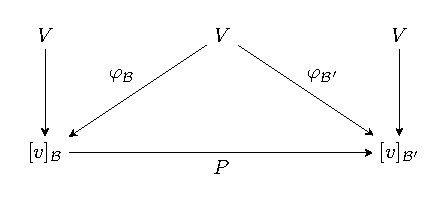
\includegraphics[width=0.4\textwidth]{diagramas_conmutativos.pdf}
        \label{fig:conexiones}
    \end{figure}

    La columna $j$ de $P$ esta dada por las coordenadas $[v]_{\BB^{\prime}}$.\\
    Sea $\R^{2}$ y $\BB=\{(1,0),(0,1)\}$ y $\BB^{\prime}=\{(1,1),(0,2)\}$ bases, veamos el siguiente
    diagrama
    
    \begin{figure}[H]
        \centering
        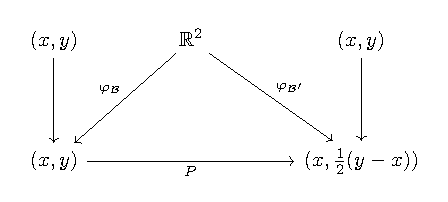
\includegraphics[width=0.4\textwidth]{diagramas_conmutativos2.pdf}
        \label{fig:conexiones2}
    \end{figure}
    Las coordenadas de $\BB$ respecto a $\BB^{\prime}$ son
    \begin{equation*}
        \begin{matrix}
            [(1,0)]_{\BB^{\prime}}=(1,-\frac{1}{2})\\
            [(0,1)]_{\BB^{\prime}}=(0,\frac{1}{2})
        \end{matrix}
        \implies P=
        \begin{pmatrix}
            1 & 0\\
            -\frac{1}{2} & \frac{1}{2}
        \end{pmatrix}
    \end{equation*}

    \begin{proposicion}
        $P\in M_{n\times n}(F)$ es invertible.
    \end{proposicion}
    
    \begin{proof}
    Tenemos que
        \begin{equation*}
            P
            \begin{pmatrix}
                x_{1}\\
                \vdots\\
                x_{n}
            \end{pmatrix}
            =
            \begin{pmatrix}
                0\\
                \vdots\\
                0
            \end{pmatrix}
        \end{equation*}
        \begin{equation*}
            P[v]_{\BB}=[v]_{\BB^{\prime}}=(0,\dots,0).
        \end{equation*}
        \begin{equation*}
            \implies v=0\implies [v]_{\BB}=(0,\dots,0).
        \end{equation*}
        Por tanto, el sistema homogeneo tiene solo la solución trivial y por lo tanto
        la matriz es invertible.
    \end{proof}

    Como $P$ es invertible entonces sus vectores columna son linealmente independientes y forman
    una base de $F^{n}$.
    
    \begin{proposicion}
        Si $\varphi_{\BB}:V\to F^{n}$ es una biyección ademas satisface lo siguiente si $v,w\in V$,
        $a\in F$ entonces
        \begin{align*}
            \varphi_{\BB}(av+w)&=a\varphi_{\BB}(v)+\varphi_{\BB}(w)\\
            [av+w]_{\BB}&=a[v]_{\BB}+[w]_{\BB}
        \end{align*}
    \end{proposicion}

    \begin{proof}
        Supongamos que
        \begin{equation*}
            v=\sum_{i=1}^{n}b_{i}v_{i},\qquad w=\sum_{i=1}^{n}c_{i}v_{i}\in V.
        \end{equation*}
        Sea $a\in F$,
        \begin{align*}
            av+w&=a\parentesis{\sum_{i=1}^{n}b_{i}v_{i}}+\parentesis{\sum_{i=1}^{n}c_{i}v_{i}}\\
            &=\sum_{i=1}^{n}(ab_{i}v_{i}+c_{i}v_{i})\\
            &=\sum_{i=1}^{n}(ab_{i}+c_{i})v_{i},
        \end{align*}
        entonces
        \begin{align*}
            [av+w]_{\BB}&=a[v]_{\BB}+[w]_{\BB}\\
            &=a(b_{1},\dots,b_{n})+(c_{1},\dots,c_{n})\\
            &=(ab_{1}+c_{1},ab_{2}+c_{2},\dots,ab_{n}+c_{n}).
        \end{align*}
    \end{proof}

    \section{Ejrecicios}

    En todos los problemas, $F$ es el campo $\Q, \R$ o $\C$.

    \begin{ejercicio}
        Sea $V$ un espacio vectorial sobre $F$. Demuestra que
        \begin{itemize}
            \item[(a)] El vector cero $0 \in V$ es único.
            \item[(b)] Para todos $v_1, v_2 \in V$, existe un único $v_3 \in V$ tal que $v_1 + v_3 = v_2$
            \item[(c)] Para todo $v \in V$, se tiene que $(-1)v = -v$ y $0v = 0$.
        \end{itemize}
    \end{ejercicio}

    \begin{ejercicio}
        Considera $V = \llaves{(x_1,x_2) : x_1,x_2 \in \C}$ y define las operaciones:
        \begin{align*}
            + : V \times V & \to V\\
            \parentesis{(x_1,x_2), (y_1, y_2)} & \mapsto (x_1 + y_1 + 1, x_2 + y_2 + 1),
        \end{align*}
        \begin{align*}
            \cdot : \C \times V & \to V\\
            (c,(x_1, x_2)) & \mapsto (cx_1 + c - 1, cx_2 + c - 1).
        \end{align*}
        ¿Es $V$ un espacio vectorial sobre $\C$ con estas operaciones?.
    \end{ejercicio}

    \begin{ejercicio}
        Considera el espacio vectorial usual $\R^n$ sobre $\R$, determina cuáles de los siguientes subconjuntos son subespacios vectoriales de $\R^n$:
        \begin{itemize}
            \item[(a)] $W = \llavesgrande{(a_1, \dots , a_n) \in \R^n: a_1 \geq 0}$.
            \item[(b)] $W = \llavesgrande{(a_1, \dots , a_n) \in \R^n:a_1 + 3a_2 = a_3}$.
            \item[(c)] $W = \llavesgrande{(a_1, \dots , a_n) \in \R^n:a_1 = a_2}$
            \item[(d)] $W = \llavesgrande{(a_1, \dots , a_n) \in \R^n: a_j \in \Q, \text{ para todo }1 \leq j \leq n}$.
        \end{itemize}
    \end{ejercicio}

    \begin{ejercicio}
        Sean $W_1, W_2$ subespacios vectoriales de un espacio vectorial $V$ sobre el campo $F$. Demuestra que si $W_1 \cup W_2$ es un espacio vectorial de $V$, entonces uno de los espacios $W_j$ está contenido en el otro.
    \end{ejercicio}

    \begin{ejercicio}
        Considera el $\R$-espacio vectorial , $V = \llaves{f:\R \to \R : f \text{ es una función continua}}$. Demuestra que la función $f(x) = \sin (x)$ no es combinación lineal de las funciones $x, x^2, x^3$.
    \end{ejercicio}

    \begin{ejercicio}
        Sea $V$ un espacio vectorial sobre un campo $F$ y sean $W_1, \dots , W_k$ subespacios vectoriales de $V$. Demuestra que
        \[
        W_1 + \dotsi + W_k := \llavesgrande{ w_1 + \dotsi + w_k: w_i \in W_i, \forall i \in \{1, \dots, k \}},
        \]
        es un subespacio vectorial de $V$.
    \end{ejercicio}

    \begin{ejercicio}
        Falso o verdadero (justifica tus respuestas: si es verdadero demuéstralo y si es falso da un contraejemplo):
        \begin{itemize}
            \item[(a)] El vacío es un subconjunto linealmente independiente.
            \item[(b)] Sea $V$ un espacio vectorial sobre $F$, si $S \subset V$ es linealmente dependiente entonces cualquier subconjunto propio de $S$ es linealmente independiente.
            \item[(c)] Sea $V$ un espacio vectorial sobre $F$, si $S \subset V$ es linealmente independiente entonces cualquier subconjunto de $S$ es linealmente independiente.
            \item[(d)] Si un conjunto de cuatro vectores en $\R^4$ es linealmente independiente, entonces necesariamente genera a $\R^4$.
        \end{itemize}
    \end{ejercicio}

    \begin{ejercicio}
        Demuestra que el espacio vectorial $V = \llaves{f: \R \to \R: f \text{ es función}}$ sobre $\R$, existe un conjunto infinito que es linealmente independiente.
    \end{ejercicio}

    \begin{ejercicio}
        Encuentra el conjunto $\llaves{v_1, v_2, v_3}$ de vectores linealmente dependientes en $\R^3$ tales que dos a dos son linealmente independientes.
    \end{ejercicio}

    \begin{ejercicio}
        Sean $a,b,c \in \R$ distintos entre sí. Demuestra que $\llaves{(1, 1, 1), (a, b, c), (a^2, b^2, c^2)}$ es linealmente independiente en $\R^3$.
    \end{ejercicio}

    \begin{ejercicio}
        Encuentra una base de $\R^3$ que contenga a los vectores $(1, 1, 1)$ y $(1, 2, 3)$, si existe. Si no existe, demuéstralo.
    \end{ejercicio}

    \begin{ejercicio}
        Encuentra una base del espacio de soluciones en $F^4$ del sistema:
        \begin{align*}
            x_1 + 4x_2 + 3x_3 - x_4 = & 0\\
            3x_1 - 5x_2 + 9x_3 - 2x_4 = & 0\\
            2x_1 - x_2 + 6x_3 - x_4 = & 0.\\
        \end{align*}
    \end{ejercicio}

    \begin{ejercicio}
        Sean $W_1$, $W_2$ subespacios vectoriales de dimensión 2 en $F^3$, demuestra que:
        \[
        \dim_F(W_1 \cap W_2) > 0.
        \]
    \end{ejercicio}

    \begin{ejercicio}
        Sea $V$ un espacio vectorial de dimensión $n$ sobre un campo $F$. Determina si las siguientes afirmaciones son falsas o verdaderas, justifica tus respuestas:
        \begin{itemize}
            \item[(a)] Para todo $v \in V$, existe una base $V$ que contiene a $v$.
            \item[(b)] Si $\llaves{v_1, \dots, v_n}$ genera a $V$, entonces es una base de $V$.
            \item[(c)] Si $S = \llaves{v_1, \dots, v_n, v_{n+1}}$ genera a $V$, entonces existe un subconjunto de $S$ con $n$ elementos que es una base de $V$.
            \item[(d)] Si $w \in V \setminus \llaves{0}$ y $\mathcal{B} = \llaves{v_1, \dots, v_n}$ es una base de $V$, entonces existe $i \in \llaves{1, \dots, n}$ tal que al reemplazar $w$ por $v_i$ en $\mathcal{B}$, seguimos teniendo una base de $V$.
        \end{itemize}
    \end{ejercicio}

    \begin{ejercicio}
        Sea $V$ un espacio vectorial sobre $F$ y sea $\llaves{v_1, v_2, v_3, v_4}$ una base de $V$. Consideramos los vectores $w_1 = v_1 + v_2$, $w_2 = v_2 + v_3$, $w_3 = v_3 + v_4$ y $w_4 = v_4 + v_1$. Encuentra la dimensión y una base del subespacio de $V$ generado por $\llaves{w_1, w_2, w_3, w_4}$. ¿Exista algún subconjunto de $\llaves{w_1, w_2, w_3, w_4}$ que sea una base de este subespacio? justifica tu respuesta.
    \end{ejercicio}

    \begin{ejercicio}
        Demuestra que el espacio vectorial $\mathcal{F} = \llaves{f: \R \to \R : f \text{ es una función continua}}$ no es un espacio de dimensión finita sobre $\R$.
    \end{ejercicio}

    \begin{ejercicio}
        Sea $W = \llaves{(x_1, \dots, x_n) \in \R^n : x_1 + 2x_2 + \dotsi + nx_n = 0}$. Demuestra que $W$ es un subespacio vectorial de $\R^n$ y encuentra una base para él.
    \end{ejercicio}

    \begin{ejercicio}
        Dado un espacio vectorial $V$ de dimensión finita $n$ sobre $F$ y dada una base ordenada $\mathcal{B}$ de $V$. Demuestra que para todo $v, w \in V$y $a \in F$, se tiene que:
        \[
        \corchetes{av + w}_\BB = a[v]_\BB + [w]_\BB.
        \]
    \end{ejercicio}

    \begin{ejercicio}
        Demuestra que $\BB = \llaves{\parentesis{1, 2, 0, 1}, \parentesis{0, 1, 1, 3}, \parentesis{2, 0, 1, 1},(1, 1, 1, 1)}$ es una base de $\R^4$. Encuentra las coordenadas de $(a, b, c, d) \in \R^4$ en la base ordenada $\BB$.
    \end{ejercicio}

    \begin{ejercicio}
        Considera $V_2$ el espacio vectorial sobre $\R$ de polinomios de grado menor o igual que 2 con coeficientes en $\R$. Sea $c \in \R \setminus \llaves{0}$, entonces $\BB_2 = \llaves{1, x + c, x^2 + c}$ es base ordenada para $W_2$. Encuentra la matriz $P$ de cambio de base de $\BB_2$ a la base ordenada $\BB_1 = \llaves{1, x, x^2}$.
    \end{ejercicio}

    \begin{ejercicio}
        Demuestra $\BB_2 = \llaves{(2i, 1, 0), (2, -1, 1), (0, 1 + i, 1 - i)}$ es una base de ordenada de $\C^3$ y encuentra la matriz de cambio de base de $\BB_2$ a la base canónica $\BB_1$.
    \end{ejercicio}

    \begin{ejercicio}
        Sea $V$ un espacio vectorial de dimensión finita $n$ sobre un campo $F$ y sean $\BB_1, \BB_2, \BB_3$ bases ordenadas de $V$. Si $P$ es la matriz de cambio de base de $\BB_2$ a $\BB_1$ y $Q$ es la matriz de cambio de base de $\BB_3$ a $\BB_2$. Encuentra la matriz de cambio de base de $\BB_3$ a $\BB_1$ en términos de $P$ y $Q$.
    \end{ejercicio}

    \begin{ejercicio}
        Sea $V = \R^3$ y considera las bases:
        \[
        \BB = \llaves{(1, 1, 0), (0, 1, 1), (1, 0, 1)}, \quad \mathcal{C} = \llaves{(2, 1, 1), (1, 1, 0), (0, 1, 1)}.
        \]
        \begin{itemize}
            \item[(a)] Calcula la matriz de cambio de base de $\mathcal{C}$ a $\BB$.
            \item[(b)] Encuentra todos los vectores $v \in \R^3$ tales que $[v]_\BB = [v]_\mathcal{C}$.
        \end{itemize}
    \end{ejercicio}

    \begin{ejercicio}
        Demuestra que para todo $a\in\mathbb{R}$, $W_{a}=\{(x_{1},x_{2},x_{3},x_{4},x_{5})\in\mathbb{R}^{5}:x_{1}+x_{2}+x_{3}=ax_{5},x_{4}=0\}$
        es un subespacio vectorial de $\mathbb{R}^{5}$. Demuestra que todo
        vector en $W_{a}$ es combinación lineal de los vectores $(a,0,0,0,1)$,
        $(-1,1,0,0,0)$, $(-1,0,1,0,0)$. (justifica tu respuesta).
    \end{ejercicio}

    \begin{ejercicio}
        Demuestra que $W=\{(x_{1},x_{2},x_{3},x_{4})\in\mathbb{R}^{4}:x_{1}x_{2}=0\}$
        no es subespacio vectorial de $\mathbb{R}^{4}$
    \end{ejercicio}

    \begin{ejercicio}
        Encuentra una base del siguiente subespacio vectorial de $\R^{4}$
        (justifica tu respuesta).
        \begin{equation*}
            W=\{(x_{1},x_{2},x_{3},x_{4})\in\R^{4}:x_{1}+x_{2}+x_{3}+x_{4}=0\}.
        \end{equation*}
    \end{ejercicio}
    
    \chapter{Transformaciones Lineales}

    \section{Transformaciones lineales}


    \begin{definicion}[Transformación Lineal]
        Sean $V,W$ espacios vectoriales sobre un campo $F$, una función $T:V\to W$ es una
        \textbf{transformación lineal} si
        \begin{equation*}
            T(av_{1}+v_{2})=aT(v_{1})+T(v_{2})
        \end{equation*}
        para todo $a\in F$ y $v_{1},v_{2}\in V$.
    \end{definicion}

    \textbf{Observación.}
    Por inducción, la condición anterior se extiende a combinaciones lineales arbitrarias:
    \begin{equation*}
        T\parentesis{\sum_{i = 1}^na_iv_i} = \sum_{i = 1}^na_iT(v_i)
    \end{equation*}
    De la definición anterior también se deducen directamente las identidades $T(0)=0$ y $T(-v)=-T(v)$, que serán útiles en las demostraciones que siguen.

    \begin{ejemplo}
        Sea $A = (a_{ij}) \in M_{m \times n}(F)$ el producto
        \begin{align*}
            A:F^n & \to F^m\\
            \begin{pmatrix}
                b_1\\
                \vdots\\
                b_n
            \end{pmatrix}
            & \mapsto A\begin{pmatrix}
                b_1\\
                \vdots\\
                b_n
            \end{pmatrix} = 
            \begin{pmatrix}
                \sum_{i = 1}^na_{1i}b_i\\
                \vdots\\
                \sum_{i = 1}^na_{mi}b_i\\
            \end{pmatrix}.
        \end{align*}
        Es una transformación lineal.
    \end{ejemplo}

    \begin{ejemplo}
        Consideremos los siguientes conjuntos.
        \begin{equation*}
            \mathcal{C} = \llaves{f:\mathbb{R} \to \mathbb{R}: f \text{ función}}
        \end{equation*}
        \begin{equation*}
            \mathcal{V} = \llaves{f: \mathbb{R} \to \mathbb{R}:f \text{ diferenciable}}
        \end{equation*}
        Sea la función
        \begin{align*}
            \mathcal{O}:\mathcal{V} & \to \mathcal{C}\\
            f(x) & \mapsto f'(x).
        \end{align*}
        Es una transformación lineal.
    \end{ejemplo}

    \begin{ejemplo}
        Sea
        \begin{equation*}
            \mathcal{W} = \llaves{f:\mathbb{R} \to \mathbb{R}:f \text{ es integrable}}.
        \end{equation*}
        Así,
        \begin{align*}
            \mathcal{I}: \mathcal{W} & \to \mathcal{W}\\
            f(x) & \mapsto \int_{0}^xf(t)dt
        \end{align*}
        es transformación lineal.
    \end{ejemplo}

    \begin{proposicion}
        Si $T:V \to W$ es una transformación lineal, entonces basta conocer la imagen en una base
        de $V$ para conocer la imagen de todo vector en $V$.
    \end{proposicion}

    \begin{proof}
        Sea la transformación lineal $T:V \to W$ y $\mathcal{B}$ una base de $V$. Supongamos que $T(v_i) = w_i$ para todo $v_i \in \mathcal{B}$. Sea $v \in V$, $v = \sum_{i = 1}^na_iv_i$, donde $a_1, \dots, a_n \in F$ y $v_1, \dots, v_n \in \mathcal{B}$. Así que
        \begin{align*}
            T(v) & = T\parentesis{\sum_{i = 1}^na_iv_i}\\
            & = \sum_{i = 1}^na_iT(v_i)\\
            & = \sum_{i = 1}^na_iw_i.
        \end{align*}
    \end{proof}

    \begin{ejemplo}
        Sean
        \begin{equation*}
            T: \mathbb{R}^{2} \to \mathbb{R}^{2},
        \end{equation*}
        $T(1,0) = (a_1, b_1)$ y $T(0, 1) = (a_2, b_2)$. Luego
        \begin{align*}
            T(x, y) & = x(a_1, b_1) + y(a_2, b_2)\\
            & = (a_1x + a_2y, b_1x + b_2y).
        \end{align*}
    \end{ejemplo}

    Sea $T:V\to W$ transformacion lineal entonces
    \begin{equation*}
        T(0)=0\quad\text{ y }\quad T(-v)=-T(v)
    \end{equation*}

    \begin{definicion}[Kernel e Imagen]
        El \textbf{espacio nulo} o \textbf{kernel}, (denotado por $\ker(T)$), es
        \begin{equation*}
            0\in\ker(T)=\{v\in V:T(v)=0_{W}\}\subset V.
        \end{equation*}
        La \textbf{imagen} de $T$ es
        \begin{equation*}
            \Im(T)=\{T(v)\in W:v\in V\}\subset W.
        \end{equation*}
    \end{definicion}

    \begin{proposicion}
        $\ker(T)$ es un subespacio vectorial de $V$ y $\Im(T)$ es un subespacio vectorial de $W$.
    \end{proposicion}

    \begin{proof}
        Basta probar que, sea $S \subset V$ es un subespacio vectorial si y solo si $S$ es no vacío y para todo $a \in F$, $v_1, v_2 \in S$ se tiene que $av_1 + v_2 \in S$.
        \begin{itemize}
            \item[(1)] Notemos que $0 \in \ker{T}$ así que es no vacío. Sean $a \in F$, $v_1, v_2 \in \ker{T}$. Luego,
            \begin{align*}
                T(av_1 + v_2) & = aT(v_1) + T(v_2)\\
                & = a \cdot 0 + 0\\
                & = 0.
            \end{align*}
            \item[(2)] Veamos que $T(0) = 0$, así que es no vacío. Sean $a \in F$, $T(v_1), T(v_2) \in \Im (T$). Dado que $aT(v_1) + T(v_2) \in \Im (T)$, al ser una transformación lineal, se sigue que $T(av_1 + v_2) \in \Im (T)$.
        \end{itemize}
    \end{proof}

    \begin{definicion}[Nulidad]
        La dimensión de $\ker(T)$ se le llamada \textbf{nulidad} de $T$. Denotada por
        \begin{equation*}
            \dim(\ker(T))=\nul(T).
        \end{equation*}
    \end{definicion}

    \begin{ejemplo}
        Sea $\mathcal{P}_n$. Tomemos la siguiente función
        \begin{align*}
            \mathcal{D}: \mathcal{P} & \to \mathcal{P}\\
            \sum_{i = 0}^na_ix^{i} & \mapsto \sum_{i = i}^nia_ix^{i-1}.
        \end{align*}
        Luego, 
        \begin{align*}
            \ker(\mathcal{D}) = \llaves{a_0:a_0 \in \mathbb{R}},\\
            \nul{\mathcal{D}} = 1.
        \end{align*}
    \end{ejemplo}

    \begin{definicion}[Rango]
        La dimensión de $\Im(T)$ de $W$ se llama \textbf{rango} de $T$. Denotada por
        \begin{equation*}
            \dim(\Im(T))=\rg(T)
        \end{equation*}
    \end{definicion}

    \begin{ejemplo}
        El rango de la transformación lineal vista en el ejemplo $3.5$ es 
    \begin{equation*}
        \Im(\mathcal{D})= \llavesgrandes{\sum_{i = 0}^{n-1}a_ix^{i}: a_i \in \mathbb{R}} \qquad \implies \qquad \rg(\mathcal{D}) = n.
    \end{equation*}
    \end{ejemplo}

    \begin{teorema}[Rango-Nulidad]
        Sean $V, W$ espacios vectoriales sobre $F$ tal que $V$ es de dimensión finita $n$. Si $T:V \to W$ es una transformación lineal, entonces
        \begin{equation*}
            \nul{T} + \rg{T} = n.
        \end{equation*}
    \end{teorema}

    \begin{proof}
        Recordemos que $\ker(T) = \llaves{v \in V: T(v) = 0}$ es un subespacio vectorial de $V$. Así $\nul{T} = k \leq n$. Sea $\mathcal{B}_1 = \llaves{v_1, \dots , v_k}$ una base de $\ker(T)$. Completamos $\mathcal{B}_1$ a una base $\mathcal{B} = \llaves{v_1, \dots,v_k, v_{k + 1}, \dots , v_n}$ de $V$. Queremos probar que $\rg{T} = n - k$. Vamos a probar que $\llaves{T(v_{k + 1}),T(v_{k + 2}), \dots, T(v_n)} \subset \Im(T)$ es una base de $\Im(T)$. Sea $T(v) \in \Im(T)$, con $v \in V$. Entonces existen escalares $a_1, \dots , a_n \in F$ tales que $v = \sum_{i = 1}^na_iv_i$, entonces
        \begin{equation*}
            T(v) = \sum_{i = 1}^n a_i T(v_i) = \sum_{i = 1}^k a_i T(v_i) + \sum_{i = k + 1}^n a_i T(v_i).
        \end{equation*}
        Como $v_1, \dots, v_k \in \ker(T)$, entonces $T(v) = \sum_{i = k + 1}^n a_i T(v_i)$. Por tanto $\llaves{T(v_{k+1}), \dots, T(v_n)}$ genera a $\Im(T)$. Supongamos que $\sum_{i = k+1}^n a_i T(v_i) = 0 = T\left(\sum_{i = k+1}^n a_i v_i\right)$. Por tanto
        \begin{equation*}
            \sum_{i = k+1}^n a_i v_i \in \ker(T).
        \end{equation*}
        Existen $c_1, \dots, c_n \in F$ tales que
        \begin{equation*}
            \sum_{i = k+1}^n a_i v_i - \sum_{i = 1}^n c_i v_i = 0.
        \end{equation*}
        Como $\llaves{v_1, \dots, v_n}$ es base, se tiene que $a_{k + 1} = \dotsi = a_n = 0$. Así que $\llaves{T(v_{k + 1}), \dots , T(v_n)}$ es base de $\Im(T)$, por tanto $\rg{T} = n - k = n - \nul{T}$. Concluyendo así que
        \begin{equation*}
            \nul{T} + \rg{T} = n.
        \end{equation*}
    \end{proof}

    \begin{ejemplo}
        Tomemos la siguiente transformación lineal,
        \begin{align*}
            T : \mathbb{R}^2 & \to \mathbb{R}^2,\\
            (x,y) & \mapsto (2x + y, 0).
        \end{align*}
        Así,
        \begin{align*}
            \ker(T) & = \llaves{(x,y):(2x + y, 0) = (0, 0)}\\
            & = \llaves{(x, -2x):x \in \mathbb{R}}\\
            & = \llaves{x(1,-2):x \in \mathbb{R}}\\
            & \implies \nul{T} = 1.
        \end{align*}
        Por otra parte, 
        \begin{align*}
            \Im(T) & = \llaves{(2x + y, 0): x, y \in \mathbb{R}}\\
            & = \llaves{(a, 0): a \in \mathbb{R}}\\
            & = \llaves{a(1,0): a \in \mathbb{R}}\\
            & \implies \rg{T} = 1
        \end{align*}
        Luego,
        \begin{equation*}
            \nul{T} + \rg{T} = \dim \mathbb{R}^2.
        \end{equation*}
    \end{ejemplo}

    \begin{ejemplo}
        Sean $A = (a_{ij}) \in M_{n \times n}$ y el sistema homogéneo siguiente
        \begin{equation*}
        A
        \begin{pmatrix}
        x_1 \\
        \vdots \\
        x_n \\
        \end{pmatrix}
        = 
        \begin{pmatrix}
        0\\
        \vdots\\
        0\\
        \end{pmatrix}.
        \end{equation*}
        Tomemos la siguiente transformación lineal
        \begin{align*}
            A:F^n & \to F^n\\
            \begin{pmatrix}
                b_1\\
                \vdots\\
                b_n
            \end{pmatrix}
            & \mapsto A
            \begin{pmatrix}
                b_1\\
                \vdots\\
                b_n
            \end{pmatrix}.
        \end{align*}
        Así, $\ker(A)$ es el espacio solución del sistema lineal asociado a $A$. Si reducimos y escalonamos la matriz $A$, obtenemos que
        \begin{itemize}
            \item $\rg{A}$ es el número de filas no cero de la matriz reducida por filas escalonada equivalente a $A$.
            \item $\nul{A}$ es la cardinalidad de variables libres.
        \end{itemize}
    \end{ejemplo}

    \begin{proposicion}
        Sea $T:V \to W$ una transformación lineal, si entonces $T$ es inyectiva si y solo si $\nul{T} = 0$.
    \end{proposicion}

    \begin{proof}
        Si $T(v_1) = T(v_2)$ entonces $T(v_1 - v_2) = 0$, así que $v_1 - v_2 \in \ker(T)$. Como $\nul{T} = 0$ entonces $\ker(T) = \llaves{0}$. Por lo tanto $v_1 = v_2$ y por ende $T$ es inyectiva. Si $T$ es inyectiva, entonces
        \begin{equation*}
            T(v) = 0 \implies v = 0.
        \end{equation*}
        Así que $\ker(T) = \llaves{0}$ y por lo tanto $\nul{T} = 0$.
    \end{proof}

    \begin{corolario}
        Sean $V$ un espacio vectorial de dimensión finita $n$ sobre $F$ y $T: V \to V$ una transformación lineal. Lo siguiente es equivalente.
        \begin{itemize}
            \item[(1)] $T$ es inyectiva.
            \item[(2)] $T$ es sobre.
            \item[(3)] $T$ es biyectiva.
        \end{itemize}
    \end{corolario}
    
    \begin{proof}
        Es claro que
        \begin{equation*}
            (3) \implies (1) \qquad \text{y} \qquad (3) \implies (2).
        \end{equation*}
        Supongamos que $T$ es inyectiva, entonces esto es equivalente a que $\nul(T) = 0$. Por tanto $\rg(T) + \nul(T) = \rg(T) = \dim_F(V)$, por lo cual
        \begin{equation*}
            \dim(\Im(T)) = \dim_F V \implies \Im(T) = V.
        \end{equation*}
        Así, $T$ es sobre. Supongamos ahora que $T$ es sobre, entonces $\rg(T) = \dim_F V$, así que $\nul(T) = \dim_F(V) - \rg(T) = 0$. Por lo tanto $T$ es inyectiva. 
    \end{proof}


    Sea $A \in M_{m \times n}$, $A$ es inyectiva si y solo si $\rg(A) = n$, la matriz reducida por filas equivalente a $A$ es $I_n$, y esto es equivalente a que $A$ es invertible.

    \begin{ejemplo}
        Tomemos el siguiente sistema
        \begin{equation*}
            \begin{pmatrix}
                2 & 3 & 4\\
                1 & 0 & 0\\
                0 & 0 & 1\\
            \end{pmatrix}
            \begin{pmatrix}
                x_1\\
                x_2\\
                x_3\\
            \end{pmatrix}
            =
            \begin{pmatrix}
                2x_1 + 3x_2 + 4x_3\\
                x_1\\
                x_3\\
            \end{pmatrix}
            =
            \begin{pmatrix}
                0\\
                0\\
                0\\
            \end{pmatrix}.
        \end{equation*}
        Por lo que $\ker(A) = \llaves{(0, 0, 0)}$, $\rg(A) = 3$, $\nul{A} = 0$.
    \end{ejemplo}

    \begin{proposicion}
        Si $T:V \to W$ es una transformación lineal biyectiva, entonces
        \begin{equation*}
            T^{-1}:W\to V,
        \end{equation*}
        es transformación lineal.
    \end{proposicion}

    \begin{proof}
        Tenemos que probar que para todo $a \in F$, $w_1, w_2 \in W$, se cumple que
        \begin{equation*}
            T^{-1}(aw_1 + w_2) = a T^{-1}(w_1) + T^{-1}(w_2).
        \end{equation*}
        Al ser $T$ lineal y biyectiva, existen únicos $v_1, v_2 \in V$ tales que
        \begin{align*}
            T(av_1 + v_2) & = aT(v_1) + T(v_2)\\
            & = aw_1 + w_2.
        \end{align*}
        Así,
        \begin{equation*}
            T^{-1}(aw_1 + w_2) = av_1 + v_2 = aT^{-1}(w_1)  + T^{-1}(w_2).
        \end{equation*}
    \end{proof}

    \section{Isomorfismo}

    \begin{definicion}[Isomorfismo Lineal]
        Una transformación lineal $T:V \to W$ biyectiva se llama \textbf{isomorfismo lineal}. En este caso diremos que $V$ es isomorfo a
        $W$ y lo denotaremos como $V \simeq W$.
    \end{definicion}

    \begin{proposicion}
        El isomorfismo lineal, define una relación de equivalencia en los espacios vectoriales sobre un campo $F$.
    \end{proposicion}

    \begin{proof}
        Veamos si es reflexiva, es decir, $V \simeq V$. Notemos que la identidad cumple que
        \begin{align*}
            Id_v: V & \to V\\
            v & \mapsto v
        \end{align*}
        siendo esta una función lineal y biyectiva, en consecuencia es reflexiva.
        Supongamos ahora que $V \simeq W$, por lo que existe $T: V \to W$ lineal y biyectiva, entonces $T^{-1}: W \to V$ es lineal y biyectiva. Así que $W \simeq V$.
        Por último, supongamos que $V_1 \simeq V_2$ y $V_2 \simeq V_3$. Existen $T_1:V_1 \to V_2$ y $T_2: V_2 \to V_3$ ambas lineales y biyectivas. Consideremos $T_2 \circ T_1: V_1 \to V_3$ siendo esta lineal y biyectiva. Por tanto $V_1 \simeq V_3$.
    \end{proof}

    Supongamos $\dim V = n$ y $V \simeq W$. Así, existe $T: V \to W$ lineal y biyectiva, lo cual implica que $\nul(T) = 0$ y $\dim V = \rg (T)$. Por ser sobreyectiva, se cumple que $\rg (T) = \dim W$. Así que
    \begin{equation*}
        V \simeq W \implies \dim V = \dim W.
    \end{equation*}

    \begin{teorema}
        Un espacio vectorial $V$ de dimensión $n$ sobre $F$ es isomorfo a $F^n$.
    \end{teorema}

    \begin{proof}
        Sea $\BB = \llaves{v_1, \dots , v_n}$ una base ordenada de $v$, la función que asigna las coordenadas 
        \begin{align*}
            \varphi_{\BB}: V & \to F^n\\
            v & \mapsto (a_1, \dots, a_n)
        \end{align*}
        donde $\Sigma_{i = 1}^n a_iv_i$ es lineal. En consecuencia $\ker (\varphi_\BB) = \llaves{0}$ y $\rg (\varphi_\BB) = n$. Así que $\Im (\varphi_\BB) = F^n$, es sobre. Por tanto es un isomorfismo lineal.
    \end{proof}

    \begin{proposicion}
        Si $V, W$ son espacios vectoriales de dimensión finita sobre un campo $F$, entonces la transformación lineal
        \begin{equation*}
            T: V \to W
        \end{equation*}
        es isomorfismo lineal si y solo si $T$ es biyectiva.
    \end{proposicion}

    \begin{proposicion}
        Si $V, W$ son espacios de dimensión finita sobre $F$, entonces son isomorfos si y solo si
        \begin{equation*}
            \dim_F(V) = \dim_F(W).
        \end{equation*}
    \end{proposicion}

    \begin{proof}
        Supongamos que $V$ y $W$ son isomorfos, por lo que existe una transformación lineal
        \begin{equation*}
            T:V \to W
        \end{equation*}
        que es biyectiva. Como $T$ es lineal, podemos aplicar el teorema rango-nulidad. Dado que $T$ es inyectiva, se tiene que
        \begin{equation*}
            \ker(T) = \{0\} \implies \nul(T) = 0.
        \end{equation*}
        Por lo tanto,
        \begin{equation*}
            \rg(T) = n.
        \end{equation*}
        Pero $\rg{T} = \dim(\Im(T))$, y como $T$ es sobreyectiva,
        \begin{equation*}
            \Im(T) = W.
        \end{equation*}
        Así,
        \begin{equation*}
            \dim(W) = \dim(\Im(T)) = \rg{T} = n.
        \end{equation*}
        Por lo tanto,
        \begin{equation*}
            m = \dim(W) = n.
        \end{equation*}
        Supongamos ahora que $\dim(V) = n$ y $\dim(W) = m$, con $m = n$.
        Sean $\{v_1,\dots,v_n\}$ una base de $V$ y la transformación lineal
        \begin{align*}
            \varphi_{\mathcal{B}}:V & \to F^{n}\\
            v & \mapsto [v]_{\mathcal{B}},
        \end{align*}
        La cual es biyectiva y en consecuencia $V \simeq F^n$. De manera análoga, sea $\mathcal{B}' = \{w_1,\dots,w_n\}$ una base de $W$ y consideremos
        \begin{align*}
            \varphi_{\mathcal{B}'}:W & \to F^n\\
            w & \mapsto [w]_{\mathcal{B}'},
        \end{align*}
        la cual también es biyectiva. Por lo tanto, $W \simeq F^n$. Así, tenemos que
        \begin{equation*}
            V \simeq F^n \quad \text{y} \quad W \simeq F^n.
        \end{equation*}
        Por la transitividad de los isomorfismos, se sigue que
        \begin{equation*}
            V \simeq W.
        \end{equation*}
        Por tanto, $V$ y $W$ son isomorfos.
    \end{proof}
    
    \begin{ejemplo}
        Sea $\mathcal{P}_n$. Con $\dim_{\mathbb{R}}(\mathcal{P}_n )= n + 1$ y la base $\BB = \llaves{1, x, x^2, \dots, x^n}$. Entonces
        \begin{align*}
            \varphi_\BB: \mathcal{P}_{n} & \to \mathbb{R}^{n + 1}\\
            \sum_{i = 0}^na_ix^{i} & \mapsto (a_0, a_1, \dots, a_n)
        \end{align*}
        es un isomorfismo lineal.
    \end{ejemplo}     

    
    \begin{ejemplo}
        Sean $T: V \to W$ una transformación lineal, $\dim V = n$, $\dim W = m$, $\BB_V = \llaves{v_1, \dots, v_n}$ y $\BB_W = \llaves{w_1, \dots, w_m}$. Notemos que 

        \begin{figure}[H]
            \centering
            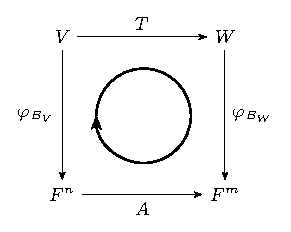
\includegraphics[width=0.4\textwidth]{diagramas_conmutativos3.pdf}
        \end{figure}
    
        En consecuencia, tenemos que 
        \begin{equation*}
            \varphi_{\BB_W} \circ T = A \circ \varphi_{\BB_V}
        \end{equation*}
        Con $A \in M_{m \times n}(F)$.
    \end{ejemplo}  

    \section{Representacion transformaciones por matrices}

    Tomemos la siguiente transformación lineal,
    \begin{align*}
        T : F^n & \to F^m\\
        e_1 & \mapsto (a_{1i}, a_{2i}, \dots , a_{mi})
    \end{align*}
    Luego,
    \begin{align*}
        (x_1, \dots, x_n) & = \sum_{i = 1}^{n}x_ie_i\\
        T(x_1, \dots, x_n) & = \sum_{i = 1}^{n}x_iT(e_i)\\
        & = \sum_{i = 1}^{n}x_i(a_{1i}, a_{2i}, \dots, a_{mi})\\
        & = \big( \sum_{i = 1}^n a_{1i}x_i, \sum_{i = 1}^n a_{2i}x_i, \dots, \sum_{i = 1}^n a_{mi}x_i \big)\\
        & = (a_{ij})
        \begin{pmatrix}
            x_1\\
            \vdots\\
            x_n
        \end{pmatrix}.
    \end{align*}
    Así, para toda transformación lineal $T:F^n \to F^m$ existe una matriz $A \in M_{m \times n}(F)$ tal que
    \begin{equation*}
        T(x_1, \dots, x_n) = A
        \begin{pmatrix}
            x_1\\
            \vdots\\
            x_n
        \end{pmatrix}.
    \end{equation*}
    Vamos a construir la matriz $A$ que satisface lo siguiente
    \begin{equation*}
        T: V \to W.
    \end{equation*}
    Sean $\BB_V = \llaves{v_1, \dots, v_n}$, $\BB_W = \llaves{w_1, \dots, w_m}$ bases ordenadas y $A \in M_{m \times n}(F)$. Notemos que
    \begin{equation*}
        A[v]_{\BB_V} = [T(v)]_{}\BB_W, \qquad \forall v \in V.
    \end{equation*}
    Luego,
    \begin{align*}
        T(v_j) = \sum_{i = 1}^na_{ij}w_i, \qquad \forall j \in \llaves{1, 2, \dots, n},\; a_{ij} \in F.\\
        \implies [T(v_j)]_{\BB_W} = (a_{1j}, a_{2j}, \dots, a_{mj}).
    \end{align*}
    Sea $v = \sum_{i = 1}^n x_j v_j \in V$, entonces
    \begin{equation*}
        T(v) = \sum_{j = 1}^{n}x_j T(v_j) = \sum_{j = 1}^n x_j \big( \sum_{i = 1}^ma_{ij}w_i \big) = \sum_{i = 1}^m \big( \sum_{j = 1}^n a_{ij}x_j \big)w_i.
    \end{equation*}
    En consecuencia
    \begin{equation*}
        [T(v)]_{\BB_W} = \big( \sum_{j = 1}^n a_{1j}x_j, \dots, \sum_{j = 1}^na_{mj}x_j \big) = A
        \begin{pmatrix}
            x_1\\
            \vdots\\
            x_n
        \end{pmatrix} = A[v]_{\BB_V},
    \end{equation*}
    donde $A = (a_{ij}) \in M_{m \times n}(F)$.

    \begin{figure}[H]
        \centering
        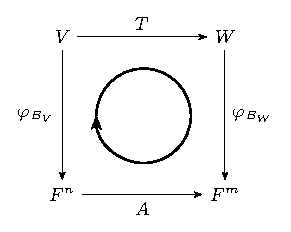
\includegraphics[width=0.4\textwidth]{diagramas_conmutativos3.pdf}
    \end{figure}

    \begin{definicion}[Representación matricial]
        La matriz $A = (a_{ij}) \in M_{m \times n}(F)$ construida anteriormente, se llama \textbf{representación matricial} de $T$ respecto a las bases $\BB_V, \BB_W$. Usaremos la siguiente notación
        \begin{gather*}
            A = [T]_{\BB_V, \BB_W}\\
            [T]_{\BB_V, \BB_W}[v]_{\BB_V} = [T(v)]_{\BB_W}.
        \end{gather*}
    \end{definicion}

    \begin{ejemplo}
        Sean
        \begin{align*}
            T: V^n & \to W^m\\
            v & \mapsto 0
        \end{align*}
        una transformación lineal y $\BB_V = \llaves{v_1, \dots, v_n}$ una base ordenada de $V$. Veamos que
        \begin{gather*}
            T(v_i) = 0 \implies [T(v)]_{\BB_V} = (0, \dots, 0) \in F^m\\
            \implies [T]_{\BB_V, \BB_W} = 0_{m \times n}.
        \end{gather*}
    \end{ejemplo}

    \begin{ejemplo}
        Sea la transformación lineal
        \begin{align*}
            T : V & \to V\\
            v & \mapsto v
        \end{align*}
        Así,
        \begin{gather*}
            T(v_i) = v_i\\
            \implies [T(v_i)]_{\BB_V} = [v_i]_{\BB_V} = e_i\\
            \implies [T]_{\BB_V} = I_n.
        \end{gather*}
    \end{ejemplo}

    \begin{ejemplo}
        Sea el espacio vectorial $\mathcal{P}_3$. Con su base ordenada $\BB = \llaves{1, x, x^2, x^3}$. Tomemos la transformación lineal
        \begin{align*}
            \mathcal{D} : \mathcal{P}_3 & \to \mathcal{P}_3\\
            \sum_{i = 0}^{3}a_ix^{i} & \mapsto \sum_{i = 0}^3ia_ix^{i - 1}
        \end{align*}
        Así,
        \begin{equation*}
            \mathcal{D}(1) = 0, \quad \mathcal{D}(x) = 1, \quad \mathcal{D}(x^2) = 2x, \quad \mathcal{D}(x^3) = 3x^2.
        \end{equation*}
        Tomemos
        \begin{align*}
            [\mathcal{D}]_{\BB}: \R^4 & \to \R^4\\
            (1, 0, 0, 0) & \mapsto (0, 0, 0, 0)\\
            (0, 1, 0, 0) & \mapsto (1, 0, 0, 0)\\
            (0, 0, 1, 0) & \mapsto (0, 2, 0, 0)\\
            (0, 0, 0, 1) & \mapsto (0, 0, 3, 0)\\
        \end{align*}
        Por tanto,
        \begin{equation*}
            [\mathcal{D}]_{\BB} = 
            \begin{pmatrix}
                0 & 1 & 0 & 0\\
                0 & 0 & 2 & 0\\
                0 & 0 & 0 & 3\\
                0 & 0 & 0 & 0
            \end{pmatrix}.
        \end{equation*}
        Tomemos ahora la base $\BB' = \llaves{1, x + 1, x^2 + 2, x^3 + 3}$, por lo que
        \begin{equation*}
            \mathcal{D}(1) = 0, \quad \mathcal{D}(x + 1) = 1, \quad \mathcal{D}(x^2 + 2) = 2x, \quad \mathcal{D}(x^3 + 3) = 3x^2.
        \end{equation*}
        Luego,
        \begin{align*}
            [\mathcal{D}]_{\BB'}: \R^4 & \to \R^4\\
            (1, 0, 0, 0) & \mapsto (0, 0, 0, 0)\\
            (0, 1, 0, 0) & \mapsto (1, 0, 0, 0)\\
            (0, 0, 1, 0) & \mapsto (-2, 2, 0, 0)\\
            (0, 0, 0, 1) & \mapsto (-6, 0, 3, 0)\\
        \end{align*}
        Por tanto,
        \begin{equation*}
            [\mathcal{D}]_{\BB'} = 
            \begin{pmatrix}
                0 & 1 & -2 & -6\\
                0 & 0 & 2 & 0\\
                0 & 0 & 0 & 3\\
                0 & 0 & 0 & 0
            \end{pmatrix}.
        \end{equation*}
    \end{ejemplo}

    \vspace{5cm}

    \begin{ejemplo}
        Tomemos las bases $\BB_{\mathcal{P}_3} = \llaves{1, x, x^2, x^3}$ y $\BB_{\mathcal{P}_4} = \llaves{1, x, x^2, x^3, x^4}$ y la siguiente transformación lineal,
        \begin{align*}
            \int : \mathcal{P}_3 & \to \mathcal{P}_4\\
            1 & \mapsto x\\
            x & \mapsto \frac{1}{2}x^2\\
            x^2 & \mapsto \frac{1}{3}x^3\\
            x^3 & \mapsto \frac{1}{4}x^4
        \end{align*}
        Lo cual implica que
        \begin{equation*}
            \big[ \int \big]_{\BB_{\mathcal{P}_3}, \BB_{\mathcal{P}_4}} =
            \begin{pmatrix}
                0 & 0 & 0 & 0\\
                1 & 0 & 0 & 0\\
                0 & \frac{1}{2} & 0 & 0\\
                0 & 0 & \frac{1}{3} & 0\\
                0 & 0 & 0 & \frac{1}{4}\\
            \end{pmatrix}
        \end{equation*}
    \end{ejemplo}

    Recapitulando, sean $V, W$ espacios vectoriales, con bases ordenadas
    \begin{equation*}
        \BB_V = \llaves{v_1, \dots , v_n}, \qquad \BB_W = \llaves{w_1, \dots w_m}
    \end{equation*}
    y la transformación lineal 
    \begin{equation*}
        T : V \to W.
    \end{equation*}
    Existe una matriz $[T]_{\BB_V, \BB_W} \in M_{m \times n}(F)$ tal que 

    \begin{figure}[H]
        \centering
        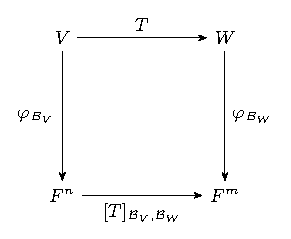
\includegraphics[width=0.4\textwidth]{diagramas_conmutativos4.pdf}
    \end{figure}

    En la columna $j \in [T]_{\BB_V, \BB_W}$ están las coordenadas de $T(v_j)$ respecto a $\BB_W$.
    \begin{equation*}
        [T(v)]_{\BB_W} = [T]_{\BB_V, \BB_W}[v]_{\BB_V}
    \end{equation*}

    \begin{proposicion}
        Sean $V_1, V_2, V_3$ espacios vectoriales con bases ordenadas $\BB_1, \BB_2, \BB_3$ respectivamente, $T_1: V_1 \to V_2$ y $T_2:V_2 \to V_3$ transformaciones lineales y $\dim V_i = n_i$. Se cumple que
        \begin{equation*}
            [T_2 \circ T_1]_{\BB_1, \BB_3} = [T_2]_{\BB_2, \BB_3}[T_1]_{\BB_1, \BB_2}
        \end{equation*}
    \end{proposicion}   

    \begin{proof}
        Podemos componer $T_2 \circ T_1: V_1 \to V_3$ obteniendo una transformación lineal. Podemos construir
        \begin{equation*}
            A = [T_1]_{\BB_1, \BB_2} \in M_{n_2 \times n_1}(F), \quad B = [T_2]_{\BB_2, \BB_3} \in M_{n_3 \times n_2}(F), \quad C = [T_2 \circ T_1]_{\BB_1, \BB_3} \in M_{n_3 \times n_1}(F)
        \end{equation*}
        Luego,
        \begin{align*}
            A[v_1]_{\BB_1} & = [T_1(v_1)]_{\BB_2}\\
            B[v_2]_{\BB_2} & = [T_2(v_2)]_{\BB_3}\\
            C[v_1]_{\BB_1} & = [T_2(T_1(v_1))]_{\BB_3}\\
            & = B[T_1(v_1)]_{\BB_2}\\
            & = B(A[v_1]_{\BB_1})\\
            & = BA[v_1]_{\BB_1}, \qquad \forall [v_1]_{\BB_1} = (x_1, \dots, x_n) \in F^n.
        \end{align*}
    \end{proof}

    \begin{teorema}
        Sean $V$ un espacio vectorial de dimensión $n$ sobre $F$ y $T: V \to V$ una transformación lineal. Si $\BB = \llaves{v_1, \dots, v_n}$ y $\BB' = \llaves{v_1', \dots, v_n'}$ son bases ordenadas de $V$, entonces
        \begin{equation*}
            P^{-1}[T]_{\BB'}P = [T]_{\BB},
        \end{equation*}
        donde $P$ es la matriz de cambio de base de $\BB$ a $\BB'$.
    \end{teorema}

    \begin{proof}
        Sabemos que existe una matriz invertible $P \in M_{n \times n}(F)$ tal que
        \[
        P[v]_\BB = [v]_{\BB'}, \qquad \forall v \in V.
        \]
        Dado que $T:V \to V$ es lineal y $[T]_{\BB'} \in M_{n \times n}(F)$, entonces tenemos que
        \begin{align*}
            [T]_{\BB}[v]_{\BB} = [T(v)]_{\BB}\\
            [T]_{\BB'}[v]_{\BB'} = [T(v)]_{\BB'}\\
        \end{align*}
        Luego,
        \begin{align*}
            [T]_{\BB'}P[v]_\BB & = P[T(v)]_{\BB}\\
            & = P[T]_{\BB}[v]_{\BB}, \qquad \forall[v]_{\BB} \in F^n
        \end{align*}
        \begin{equation*}
            \implies [T]_{\BB'}P = P[T]_{\BB} \iff P^{-1}[T]_{\BB'}P = [T]_{\BB}.
        \end{equation*}
        De manera similar podemos probar que si $Q$ es una matriz invertible de tamaño $n \times n$, entonces
        \begin{equation*}
            Q[T]_{\BB}Q^{-1} = [T]_{\BB'}.
        \end{equation*}
    \end{proof}

    \begin{figure}[H]
        \centering
        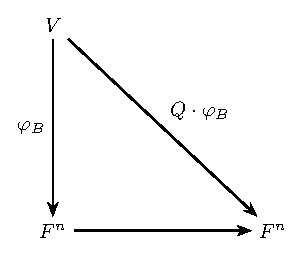
\includegraphics[width=0.4\textwidth]{diagramas_conmutativos5.pdf}
    \end{figure}

    \begin{definicion}[Matrices conjugadas]
        Sean $A, B \in M_{n \times n}(F)$ diremos que $A$ es \textbf{conjugada} con B si existe $P \in M_{n \times n }(F)$ invertible tal que
        \begin{equation*}
            A = PBP^{-1}.
        \end{equation*}
    \end{definicion}

    \begin{proposicion}
        La definición anterior, define una relación de equivalencia en $M_{n \times n}(F)$.
    \end{proposicion}
    
    \begin{proof}
        Es reflexiva, ya que $A = I_n A I_n^{-1}$. También es simétrica, a causa de que si $A = PBP^{-1}$, entonces $B = P^{-1}AP$. Por último, supongamos que $A = PBP^{-1}$ y $B = {QCQ^{-1}}$, entonces
        \begin{equation*}
            A = P(QCQ^{-1})P^{-1} = (PQ)C(PQ)^{-1}.
        \end{equation*}
    \end{proof}

    \vspace{1.2cm}

    \begin{ejemplo}
        Sea $T:\R^2 \to \R^2$ una transformación lineal dada por $T(x,y) = (-y, x + y)$. Tomemos las bases ordenadas $\BB = \llaves{(1,0), (0, 1)}$ y $\BB' = \llaves{(1, 0), (1, 1)}$.
        Construyamos la matriz $P$ de cambio de base de $\BB$ a $\BB'$, teniendo
        \begin{gather*}
            (1, 0) = 1(1,0) + 0(1, 1)\\
            (0, 1) = -1(1, 0) + 1(1, 1)\\
        \end{gather*}
        \begin{equation*}
            \implies P =
            \begin{pmatrix}
                1 & -1\\
                0 & 1\\
            \end{pmatrix}.
        \end{equation*}
        Luego,
        \begin{gather*}
            T(1,0) = (0,1)\\
            T(0,1) = (-1,1)\\
            \implies [T]_\BB =
            \begin{pmatrix}
                0 & -1 \\
                1 & 1
            \end{pmatrix}
        \end{gather*}
        y
        \begin{gather*}
            T(1,0) = (0,1) = -1(1,0) + (1,1)\\
            T(1,1) = (-1, 2) = -3(1, 0) + 2(1, 1)\\
            \implies [T]_{\BB'} =
            \begin{pmatrix}
                -1 & -3 \\
                1 & 2 \\
            \end{pmatrix}
        \end{gather*}
        Por tanto, se cumple que
        \begin{equation*}
            [T]_{\BB'}P = P[T]_{\BB} \implies [T]_{\BB'} = P[T]_{\BB}P^{-1}.
        \end{equation*}
    \end{ejemplo}

    \section{Funciones Lineales}

    Sean $V, W$ espacios vectoriales sobre $F$. Definimos
    \begin{equation*}
        \mathcal{L}(V, W) = \llaves{T:V \to W |\;\;T \text{\; es lineal }}
    \end{equation*}
    Con las operaciones
    \begin{equation*}
        \begin{aligned}
            +:\mathcal{L}(V,W)\times\mathcal{L}(V,W) & \longrightarrow \mathcal{L}(V,W) \\
            (T_{1},T_{2}) & \longmapsto T_{1}+T_{2}:V\longrightarrow W \\
            &\hspace{2.6cm} v\longmapsto T_{1}(v)+T_{2}(v).
        \end{aligned}
    \end{equation*}
    y
    \begin{equation*}
        \begin{aligned}
            \cdot: F \times\mathcal{L}(V,W)
            &\longrightarrow \mathcal{L}(V,W) \\
            (c,T)
            &\longmapsto cT:V\longrightarrow W \\
            &\hspace{1.6cm} v\longmapsto cT(v).
        \end{aligned}
    \end{equation*}
    le damos estructura de espacio vectorial sobre $F$ a $\mathcal{L}(V,W)$.

    \begin{teorema}
        Sean $V, W$ espacios vectoriales sobre $F$ de dimensión $\dim_FV = n$ y $\dim_FW = m$; y las bases ordenadas $\BB_V = \llaves{v_1, \dots, v_n}$ y $\BB_W = \llaves{w_1, \dots, w_m}$. La función
        \begin{align*}
            \Phi_{\BB_V, \BB_W}: \mathcal{L}(V, W) & \to M_{n \times n}(F)\\
            T & \mapsto [T]_{\BB_V, \BB_W} 
        \end{align*}
        Es un isomorfismo lineal.
    \end{teorema}

    \begin{proof}
        Veamos si es transformación lineal. Notemos que
        \begin{align*}
            \Phi_{\BB_v, \BB_w}(cT_1 + T_2) & = c[T_1]_{\BB_V,\BB_W} + [T_2]_{\BB_V,\BB_W}
        \end{align*}
        pues $[(cT_1 + T_2)(v_j)]_{\BB_W} = c[T_1(v_j)]_{\BB_W} + [T_2(v_j)]_{\BB_W}$. Por lo tanto es una transformación lineal. Para ver que es biyectiva, tenemos que
        \begin{equation*}
            \ker(\Phi_{\BB_V, \BB_W}) = \llaves{T \in \mathcal{L}(V, W) : [T]_{\BB_V, \BB_W} = 0_{m \times n}} = \llaves{0},
        \end{equation*}
        lo cual implica que es inyectiva. Veamos si $\Phi_{\BB_V, \BB_W}$ es sobreyectiva, dada $A = (a_{ij}) \in M_{m \times n}(F)$, tomemos la función
        \[
        \varphi_{\BB_W}: W \to F^m.
        \]
        Definimos $T(v_j) = \varphi_{\BB_W}^{-1}(a_{1j}, a_{2j}, \dots, a_{mj})$, entonces
        \[
        [T]_{\BB_V, \BB_W} = A.
        \]
        En consecuencia, $\Phi_{\BB_V, \BB_W}$ es un isomorfismo lineal.
    \end{proof}
    
    \begin{figure}[H]
        \centering
        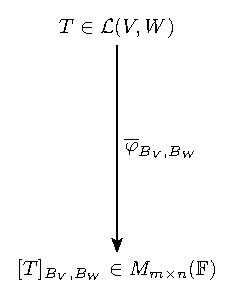
\includegraphics[width=0.2\textwidth]{diagramas_conmutativos6.pdf}
    \end{figure}

    Notemos que
    \begin{gather*}
        \dim_F \mathcal{L}(V, W) = (\dim_FV) \cdot (\dim_FW),\\
        \dim_FM_{m \times n}(F) = \dim_FF^{m \cdot n} = m \cdot n.
    \end{gather*}


    \begin{definicion}[Espacio vectorial dual]
        Sea $V$ un espacio vectorial sobre $F$, el \textbf{espacio vectorial dual de $V$} es por definición
        \begin{equation*}
            V^{*} \coloneqq \mathcal{L}(V, F) = \llaves{f:V \to F | \;\; f \text{ es lineal }}.
        \end{equation*}
        Los elementos en $V^{*}$ se llaman \textbf{funciones lineales de $V$}.
    \end{definicion}

    \begin{ejemplo}
        Sea la función
        \begin{align*}
            f: \R^2 & \to \R\\
            (x, y) & \mapsto x + y
        \end{align*}
        Veamos que
        \begin{align*}
            f(c(x_1, y_1) + (x_2, y_2)) & = f(cx_1 + x_2, cy_1 + y_2)\\
            & = cx_1 + x_2 + cy_1 + y_2\\
            & = c(x_1 + y_1) + (x_2 + y_2)\\
            & = cf(x_1, y_1) + f(x_2, y_2).
        \end{align*}
        Por tanto $f$ es una transformación lineal y en consecuencia $f \in (\R^2)^{*}$
    \end{ejemplo}

    \begin{ejemplo}
        Sea el conjunto $\mathcal{I}= \llaves{g:\R \to \R |\; g \text{ es integrable }}$. Tomemos la función
        \begin{align*}
            \int: \mathcal{I} & \to \R \\
            g & \mapsto \int_a^bg.
        \end{align*}
        Notemos que 
        \begin{equation*}
            \int(cg_1 + g_2) = c \int_a^bg_1 + \int_a^bg_2.
        \end{equation*}
        Lo cual implica que $\int \in \mathcal{I}^*$.
    \end{ejemplo}

    \vspace{1.6cm}

    \begin{ejemplo}
        Tomemos el conjunto $D = \llaves{h: \R \to \R | \; h \text{ es diferenciable en }0 \;}$, entonces, dada la función
        \begin{align*}
            f: D & \to \R\\
            g(x) & \mapsto g'(0),
        \end{align*}
        podemos afirmar que $f \in D^{*}$.
    \end{ejemplo}


    \textbf{Observación.} Si $\dim_FV = n$, entonces
    \begin{equation*}
        \dim_FV^{*} = \dim_F\mathcal{L}(V, F) = \dim_FV \cdot \dim_FF = n \cdot 1 = n.
    \end{equation*}

    \begin{definicion}[Traza]
        Definimos la \textbf{traza} de una matriz cuadrada como
        \begin{align*}
            \Tr: M_{n \times n}(F) & \to F\\
            (a_{ij}) & \mapsto \sum_{i = 1}^na_{ii}.
        \end{align*}
    \end{definicion}

    \begin{proposicion}
        La función $\Tr$ pertenece a $(M_{n \times n}(F))^*$.
    \end{proposicion}

    \begin{proof}
        Fijémonos en las siguientes igualdades,
        \begin{align*}
            \Tr (c(a_{ij}) + (b_{ij})) & = \Tr((ca_{ij} + b_{ij}))\\
            & = \sum_{i = 1}^{n}(ca_{ii} + b_{ii})\\
            & = c\sum_{i = 1}^n a_{ii} + \sum_{i = 1}^{n}b_{ii}\\
            & = c \Tr(a_{ij}) + \Tr(b_{ij})
        \end{align*}
        Por tanto es lineal y en consecuencia $\Tr \in (M_{n \times n}(F))^*$.
    \end{proof}

    \begin{ejemplo}
        Sean $v \in V$ y la función
        \begin{align*}
            \varphi_{V}: V^{*} & \longrightarrow F\\
            f & \longmapsto f(v)
        \end{align*}
        Notemos que
        \begin{align*}
            \varphi_{V}(cf_1 + f_2) & = (cf_1 + f_2)(v)\\
            & = cf_1(v) + f_2(v)\\
            & = c\varphi_V(f_1) + \varphi_V(f_2),
        \end{align*}
        por tanto $\varphi_V \in V^{*^*}$.
    \end{ejemplo}

    \begin{proposicion}
        Todo funcional lineal en $(F^n)^{\ast}$ es de la forma:
        \begin{align*}
            F^n & \to F,\\
            (x_1, \dots, x_n) & \mapsto \sum_{i = 1}^{n}a_ix_i,
        \end{align*}
        donde $a_1, \dots, a_n \in F$.
    \end{proposicion}

    \begin{proof}
        La demostración queda como ejercicio para el lector. :)
    \end{proof}


    Si $\BB = \llaves{v_1, \dots, v_n}$ es una base ordenada de $V$. Definimos la transformación lineal
    \begin{align*}
        f_i: V & \longrightarrow F\\
        v_j & \longmapsto \delta_{ij} = 
        \begin{cases}
            1 \quad \text{si } \; i = j,\\
            0 \quad \text{si } \; i \neq j.
        \end{cases}
    \end{align*}
    Sea $v = \sum_{j = 1}^n a_jv_j$ un vector cualquiera de $V$, entonces
    \begin{align*}
        f_i(v) & = f_i\parentesis{\sum_{j = 1}^na_jv_j}\\
        & = f_i\parentesis{\sum_{j = 1}^na_jf_i(v_j)}\\
        & = \sum_{j = 1}^na_j\delta_{ij}\\
        & = a_i.
    \end{align*}
    Así, $f_i$ manda el vector $v$ a la cordenada $i$-ésima respecto a $\BB$.

    \begin{proposicion}
        Las funciones $\llaves{f_1, \dots, f_n}$ forman una base de $V^{*}$.
    \end{proposicion}
    
    \begin{proof}
        Sabemos que $\dim_FV = \dim_{F}V^{*}$, basta probar que $\llaves{f_1, \dots, f_n}$ son linealmente independientes. Sean $c_i, \dots, c_n \in F$, tales que 
        \begin{gather*}
            c_1f_1 + \dots + c_nf_n = 0\\
            \implies0= \sum_{i = 1}^nc_if_i(v_j) = \sum_{i = 1}^{n}c_if_i(v_j) = \sum_{i = 1}^{n}c_i \delta_{ij} = c_j\\
            \implies c_j = 0.
        \end{gather*}
        Así, $\llaves{f_1, \dots, f_n}$ es una base de $V^{*}$.
    \end{proof}

    \begin{definicion}[Base dual]
        Si $\BB = \llaves{v_1, \dots, v_n}$ es una base ordenada de $V$, entonces
        \[
        \llaves{f_1, \dots, f_n} \subset V^{*}
        \]
        definidas mediante
        \begin{align*}
            f_i: V & \longrightarrow F\\
            v_j & \longmapsto \delta_{ij}
        \end{align*}
        forman una base ordenada de $V^*$, la cual llamaremos \textbf{base dual de $\BB$}, se denota por 
        \[
        \BB^* = \llaves{f_1, \dots, f_n}.
        \]
    \end{definicion}
    
    \textbf{Ejemplo.} Sean el espacio vectorial $V = \llaves{\sum_{i = 0}^na_ix^{i}:\; a_i \in \R}$ y la base ordenada $\BB = \llaves{1, x, x^2, \dots, x^n}$. Construyamos la base dual $\BB$ de $V^*$. Notemos que
    \begin{align*}
        f_i: V & \longrightarrow F\\
        x^j & \longmapsto \delta_{ij}.
    \end{align*}
    Luego,
    \[
    f\parentesis{\sum_{k = 0}^na_kx^k} = \sum_{k = 0}^{n}a_k\delta_{ik} = a_i
    \]
    Por lo cual, $\BB^* = \llaves{f_0, f_1, \dots, f_n}$. \hfill $\blacktriangleleft$

    Sea $V$ un espacio vectorial, tomemos $v \in V$, podemos definir
    \begin{align*}
        \varphi_v: V^* & \longrightarrow F\\
        f & \longmapsto f(v)
    \end{align*}
    Siendo esta una transformación lineal, ya que
    \begin{align*}
        \varphi_v(af_1 + f_2) & = (af_1 + f_2)(v)\\
        & = af_1(v) + f_2(v)\\
        & = a \varphi_v(f_1) + \varphi_v(f_2).
    \end{align*}
    Así que $\varphi_v \in V^{*^*}$.

    \begin{teorema}
        Sea $V$ un espacio vectorial de dimensión finita $n$, entonces la función
        \begin{align*}
            \varphi: V & \longrightarrow V^{*^*}\\
            v & \longmapsto \varphi_v\\[12pt]
            &\varphi_v \coloneqq \varphi(v).
        \end{align*}
        Es un isomorfismo lineal.
    \end{teorema}
    
    \begin{proof}
        Por lo visto anteriormente, sabemos que está bien definida, ya que $\varphi_v \in V^{*^*}$. Veamos que $\varphi$ es lineal. Sea $f \in V^{*^*}$, entonces 
        \begin{align*}
            \varphi_{av_1 + v_2}(f) & = f(av_i + v_2)\\
            & = af(v_1) + f({v_2})\\
            & = a \varphi_{v_1}(f) + \varphi_{v_2}(f)\\
            & = (a\varphi_{v_1} + \varphi_2)(f).
        \end{align*}
        Así que $\varphi_{av_1 + v_2} = a\varphi_1 + \varphi_2$. Por último probemos la biyectividad de $\varphi$. Notemos que
        \[
        \dim_FV = \dim_FV^* = \dim_FV^{*^*}.
        \]
        Como tienen la misma dimensión el dominio y el contradominio, se sigue que $\varphi$ es sobreyectiva. Basta ver que $\nul \varphi = 0$, para probar que es isomorfismo lineal. Veamos que 
        \[
        \ker (\varphi) = \llaves{v \in V : \varphi_v = 0}.
        \]
        Sea $\BB = \llaves{v_1, \dots, v_n}$ una base de $V$, entonces para $f_i(v) = 0$ es la $i$-ésima coordenada de $v$ en $\BB$. Así que $v = 0$. Concluyendo que
        \begin{align*}
        \varphi: V & \longrightarrow V^{*^*}\\
        v & \longmapsto \varphi_v\\
        \end{align*}
        es un isomorfismo, en especial uno canónico, es decir, no depende de las bases.
    \end{proof}

    \section{Transpuesta de una transformación lineal}

    \begin{definicion}[Matriz transpuesta]
        Sea $A = (a_{ij}) \in M_{m \times n}(F)$. La \textbf{matriz transpuesta} de $A$, se define como
        \[
        A^t = (a_{ji}) \in M_{n \times m}(F).
        \]
    \end{definicion}


    \textbf{Ejemplo.} Veamos los siguientes ejemplos.
    \[
    \begin{pmatrix}
        a_{11} & a_{12}\\
        a_{21} & a_{22}\\
    \end{pmatrix}^t = 
    \begin{pmatrix}
        a_{11} & a_{21}\\
        a_{12} & a_{22}\\
    \end{pmatrix}.
    \]
    \[
    \begin{pmatrix}
        a_{11}\\a_{21}
    \end{pmatrix}^t = 
    \begin{pmatrix}
        a_{11} & a_{21}
    \end{pmatrix}.
    \]
    \[
    I_n^t = I_n.
    \]
    \[
    \begin{pmatrix}
        1 & 2\\
        3 & 5\\
        0 & 1\\
    \end{pmatrix}^t =
    \begin{pmatrix}
        1 & 3 & 0\\
        2 & 5 & 1
    \end{pmatrix}.
    \]
    \hfill $\blacktriangleleft$

    Si $V, W$ son espacios vectoriales de dimensión $m$ y $n$ respectivamente y sus bases ordenadas $\BB_V = \llaves{v_1, \dots, v_n}$ y $\BB_W = \llaves{w_1, \dots, w_m}$. Tomemos la transformación lineal $T: V \to W$ y la representación matricial $[T]_{\BB_V, \BB_W} = A \in M_{m \times n}(F)$. Podemos definir
    \begin{equation*}
        \begin{aligned}
            T^*: W^* & \longrightarrow V^* \\
            g & \longmapsto g \circ T:V\longrightarrow F \\
            &\hspace{2.1cm} v\longmapsto g(T(v)).
        \end{aligned}
    \end{equation*}
    La cual resulta ser lineal, ya que $T^*$ es composición de lineales. También, tenemos que
    \[
    \ker(T^*) = \llaves{g \in W^* : g \circ T = 0}.
    \]
    Por otro lado,
    \[
    \Im (T^*) = \llaves{g \circ T : g \in W^*}.
    \]
    Por el teorema de rango-nulidad, tenemos que
    \[
    \ker (T^*) + \rg (T^*) = \dim W.
    \]

    \vspace{1.8cm}

    \begin{definicion}[Transformación dual]
        A la función
        \[
        T^*: W^*  \longrightarrow V^*
        \]
        se le llama \textbf{transformación dual de $T$}.
    \end{definicion}

    \begin{teorema}
        Sean $V, W$ de espacios vectoriales de dimensiones $n$ y $m$ respectivamente, y sus bases $\BB_V = \llaves{v_1, \dots, v_n}$ y $\BB_W = \llaves{w_1, \dots, w_m}$ y la transformación lineal $T: V \to W$ junto con su transformación dual
        \[
        T^* : W^* \longrightarrow V^*.
        \]
        Sea $A = (a_{ij}) = [T]_{\BB_V, \BB_W} \in M_{m \times n}(F)$, entonces se cumple que
        \[
        [T^*]_{\BB_W^*, \BB_{V}^*} = A^t = [T]^t_{\BB_V, \BB_W} = (a_{ji}) \in M_{n \times m}(F).
        \]
        Con las bases $\BB_{V}^* = \llaves{f_1, \dots, f_n}$ y $\BB_{W}^* = \llaves{g_1, \dots, g_m}$, donde $f_i(v_j) = \delta_{ij}$ y $g_i(w_i) = \delta_{ij}$.
    \end{teorema}
    
    \begin{proof}
        Sea $[T]_{\BB_V, \BB_W} = (a_{ij})$, entonces
        \[
        T(v_j) = \sum_{i = 1}^ma_{ij}w_i.
        \]
        Tomemos $[T^*]_{\BB^*_W, \BB^*_V} = (b_{ij}) \in M_{n \times m}(F)$, entonces
        \[
        T^*(g_j) = \sum_{i = 1}^nb_{ij}f_i.
        \]
        Por otro lado,
        \begin{align*}
            T^*(g_j)(v_i) & = (g_j \circ T)(v_i)\\
            & = g_j(T(v_i))\\
            & = g_j\parentesis{\sum_{k = 1}^ma_{ki}w_k}\\
            & = \sum_{k = 1}^ma_{ki}g_j(w_k)\\
            & = \sum_{k = 1}^ma_{ki}\delta_{jk}\\
            & = (a_{ji}).
        \end{align*}
        Dado $f \in V^*$, tenemos que $f = \sum_{i = 1}^n \alpha_if_i$. Luego,
        \begin{align*}
            f(v_j) & = \sum_{i = 1}^n \alpha_if_i(v_j)\\
            & = \sum_{i = 1}^n \alpha_i \delta_{ij}\\
            & = \alpha_j.
        \end{align*}
        Así,
        \[
        f = \sum_{i = 1}^nf(v_i)f_i.
        \]
        De lo anterior, obtuvimos que
        \[
        T^*(g_j)(v_i) = a_{ij} \quad \text{ y } \quad f = \sum_{i = 1}^nf(v_i)f_i, \quad \forall f \in V^*.
        \]
        En consecuencia,
        \[
        T^*(g_j) = \sum_{i = 1}^n(T^*(g_j))(v_i)f_i = \sum_{i = 1}^na_{ji}f_i.
        \]
        Concluyendo que
        \begin{gather*}
            (b_{ij}) = (a_{ji}),\\
            \implies [T^*]_{\BB^*_V, \BB^*_W} = [T]^t_{\BB_V, \BB_W}.
        \end{gather*}
    \end{proof}

    \begin{figure}[H]
        \centering
        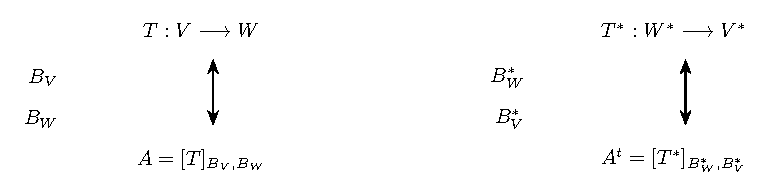
\includegraphics[width=0.9\textwidth]{diagramas_conmutativos7.pdf}
    \end{figure}

    \begin{ejemplo}
        Tomemos
        \begin{align*}
            T: \R^2 & \longrightarrow \R^3\\
            (x, y) & \longmapsto (x + y, y, 2x)
        \end{align*}
        y su transformación dual
        \begin{align*}
            T^* : (\R^3)^* & \longrightarrow (\R^2)^*\\
            g & \longmapsto g \circ T: \R^2 \longrightarrow \R.
        \end{align*}
        Sean $\BB_{2} = \llaves{e_1, e_2}$ base canónica de $\R^2$ y $\BB_3 = \llaves{\varepsilon_1, \varepsilon_2, \varepsilon_3}$ base canónica de $\R^3$. Definamos las bases duales
        $\BB_2^* = \llaves{f_1, f_2}$ dadas por
        \begin{align*}
            f_1: \R^2 & \longrightarrow \R\\
            (x, y) & \longmapsto x\\[12pt]
            f_2: \R^2 & \longrightarrow \R\\
            (x, y) &  \longmapsto y,
        \end{align*}
        y $\BB_3^* = \llaves{g_1, g_2, g_3}$, donde
        \begin{align*}
            g_1: \R^3 & \longrightarrow \R\\
            (x, y, z) & \longmapsto x\\[12pt]
            g_2: \R^3 & \longrightarrow \R\\
            (x, y, z) & \longmapsto y\\[12pt]
            g_3: \R^3 & \longrightarrow \R\\
            (x, y, z) & \longmapsto z\\[12pt]
        \end{align*}
        Por otra parte, como $T(e_1) = (1, 0, 2)$ y $T(e_2) = (1, 1, 0)$, se sigue que
        \[
        [T]_{\BB_2, \BB_3} = 
        \begin{pmatrix}
            1 & 1\\
            0 & 1\\
            2 & 0\\
        \end{pmatrix}.
        \]
        Por el teorema anterior, se colige que
        \[
        [T^*]_{\BB^*_3, \BB_2^*} = 
        \begin{pmatrix}
            1 & 0 & 2\\
            1 & 1 & 0\\
        \end{pmatrix}.
        \]
        Notemos ahora que
        \begin{equation*}
            \begin{aligned}
                T^*: (\R^3)^* & \longrightarrow (\R^2)^* \\
                g_1 & \longmapsto g_1 \circ T: \R^2 \longrightarrow \R\\
                &\hspace{1.9cm}   (x, y)\longmapsto (x + y, y, 2x) \longmapsto x + y
            \end{aligned}
        \end{equation*}
        Por lo cual $T^*(g_1) = f_1 + f_2$. De manera análoga, haciendo sus respectivos cambios, conseguimos que $T^*(g_2) = f_2$ y $T^*(g_3) = 2f_1$.
    \end{ejemplo}


    Sean $T_1: V \to V$ y $T_2: V \to V$ transformaciones lineales, entonces se cumple que
    \begin{align*}
        (T_1 \circ T_2)^*: V^* & \longrightarrow V^*\\
        f & \longmapsto f \circ(T_1 \circ T_2)\\
        & \hspace{0.6cm} = (f \circ T_1) \circ T_2\\
        & \hspace{0.6cm} = (T_1^*(f)) \circ T_2\\
        & \hspace{0.6cm} = T^*_2(T_1^*(f))
    \end{align*}
    Luego,
    \begin{align*}
        [T_2^* \circ T_1^*]_{\BB_V^*} & = [T_2^*]_{\BB_V^*}[T_1^*]_{\BB_V^*}\\
        & = [T_2]^t_{\BB_V}[T_1]^t_{\BB_V}\\
        & = ([T_1]_{\BB_V}[T_2]_{\BB_V})^t.
    \end{align*}

    \section{Ejercicios}

    En todos los problemas, $F$ es el campo $\Q, \R$ o $\C$.

    \begin{ejercicio}
        Determina cuales de las siguientes funciones $T$ de $\R^2$ a $\R^2$ son transformaciones lineales:
        \begin{itemize}
            \item[(a)] $T(x_1, x_2) = \parentesis{1 + x_1, x_2}$.
            \item[(b)] $T(x_1, x_2) = \parentesis{x_2, x_1}$.
            \item[(c)] $T(x_1, x_2) = \parentesis{x_1 + 2x_2, x_1 - 4x_2}$.
            \item[(d)] $T(x_1, x_2) = \parentesis{\sin(x_1), \sin (x_2)}$.
        \end{itemize}
        Justifica tus respuestas.
    \end{ejercicio}

    \begin{ejercicio}
        ¿Existe alguna transformación lineal de $\R^3$ en $\R^2$ tal que $T(2, 2, 2) = (2, 0)$ y $T(1, 1, 1) = (0, 1)$?
    \end{ejercicio}

    \begin{ejercicio}
        Sea $T: \R^3 \to \R^3$ tal que $T(1, 0, 0) = (0, 0, 1)$, $T(1, 1, 0) = (1, 1, 1)$ y $T(1, 1, 1) = (1, 1, 0)$.
        \begin{itemize}
            \item[(a)] Encuentra $T(x_1, x_2, x_3)$.
            \item[(b)] Encuentra el espacio nulo, imagen, nulidad y rango de $T$.
        \end{itemize}
    \end{ejercicio}

    \begin{ejercicio}
        Sean $V_1, V_2, V_3$ espacios vectoriales sobre $F$. Sean $T_1:V_1 \to V_2$ y $T_2: V_2 \to V_3$, transformaciones lineales. Demuestra que $T_2 \circ T_1 : V_1 \to V_3$ es una transformación lineal.
    \end{ejercicio}

    \begin{ejercicio}
        Sea $V$ un espacio vectorial de dimensión finita $n$ sobre $F$ y sea $T: V \to V$ una transformación lineal tal que $\Im {T} = \ker {T}$. Demuestra que $n$ es par y construye un ejemplo de una transformación lineal con esta propiedad.
    \end{ejercicio}

    \begin{ejercicio}
        Sea $V$ un espacio vectorial de dimensión $n$ sobre el campo $F$ y sea $\mathcal{B} = \llaves{v_1, \dots, v_n}$ una base ordenada de $V$. Definimos la transformación lineal $T:V \to V$ mediante $T(v_j) = v_{j + 1}$ para $j = 1, \dots, n-1$ y $T(v_n) = 0$. Demuestra que $T^n = 0$ y $T^{n-1} \neq 0$.
    \end{ejercicio}
    
    \begin{ejercicio}
        Sea $\mathcal{P}_3$ el espacio vectorial sobre $\R$ de polinomios de grado menor o igual a 3 con coeficientes en $\R$. Considera la función:
        \begin{align*}
            T: \mathcal{P}_3 & \to \R^4\\
            f(x) & \mapsto \parentesis{f(1), f(2), f(3), f(4)}.
        \end{align*}
        \begin{itemize}
            \item[(a)] Demuestra que $T$ es lineal.
            \item[(b)] Usa el teorema de rango nulidad para demostrar que para todos $a_1, a_2, a_3, a_4 \in \R$, existe $f(x) \in \mathcal{P}_3$ tal que $f(j) = a_j$ para todo $j = 1, 2, 3, 4$.
        \end{itemize}
    \end{ejercicio}

    \begin{ejercicio}
        Sea $A$ una matriz $m \times n$ con coeficientes en $F$. Demuestra que
        \begin{itemize}
            \item[(a)] El rango de filas de $A$ (que por definición es \textbf{la dimensión del subespacio vectorial que generan las filas de} $A$ vistas como vectores en $F^n$) más la dimensión del espacio de soluciones del sistema homogéneo asociado a $A$ es $n$.
            \item[(b)] Si el rango de filas de $A$ es $n$, entonces $AX = 0$ tiene solo la solución trivial.
            \item[(c)] Si el rango de filas de $A$ es menor que $n$, entonces $AX = 0$ tiene una infinidad de soluciones.
        \end{itemize}
    \end{ejercicio}
    
    \begin{ejercicio}
        Sean $V$ y $W$ espacios vectoriales de dimensión finita sobre $F$ y sea $T: V \to W$ una transformación lineal. Demuestra que $T$ es isomorfismo lineal si y solo si, para toda base $\mathcal{B}_V = \llaves{v_1, \dots, v_n}$ de $V$ se tiene que $\mathcal{B}_W = \llaves{T(v_1), \dots, T(v_n)}$ es base de $W$.
    \end{ejercicio}

    \begin{ejercicio}
        Sea $T: \R^3 \to \R^3$ definido por $(x_1, x_2, x_3) \mapsto (3x_1, x_1 - x_2, 2x_1 + x_2 + x_3)$. ¿Es $T$ isomorfismo lineal?. Si es así, encuentra $T^{-1}$.
    \end{ejercicio}

    \begin{ejercicio}
        Sean $V$ y $W$ espacios vectoriales sobre $F$, de dimensiones $n$ y $m$, respectivamente. Demuestra que $V$ y $W$ son isomorfismos si y solo si $m = n$.
    \end{ejercicio}

    \begin{ejercicio}
        Sea $V$ un espacio vectorial de dimensión finita sobre $F$ y sea $T: V \to V$. Demuestra que $T$ es isomorfismo si y solo si para alguna base ordenada $\mathcal{B}$ de $V$ se tiene que $[T]_\mathcal{B}$ es una matriz invertible.
    \end{ejercicio}

    \begin{ejercicio}
        Encuentra una base de $\Im (T)$ y de $\ker (T)$ donde $T: \R^3 \to \R^3$ está dada por:
        \[
        \begin{pmatrix}
            -1 & 2 & 1\\
            0 & 1 & 1\\
            1 & 3 & 4\\
        \end{pmatrix}.
        \]
    \end{ejercicio}

    \begin{ejercicio}
        Sea $V_2$ el espacio vectorial sobre $F$, de polinomios de grado $\leq 2$ y considera la transformación lineal
        \begin{align*}
            T : V_2 & \to F^3,\\
            a_0 + a_1x + a_2x^2 & \mapsto (a_0, a_1, a_2).
        \end{align*}
        Sean $\BB_1 = \llaves{1, x, x^2}$ y $\BB_2 = \llaves{e_1, e_2, e_3}$ bases ordenadas de $V_2$ y $F^3$. Encuentra $[T]_{\BB_1, \BB_2}$.
    \end{ejercicio}

    \begin{ejercicio}
        Sea $V = \llaves{f: \R \to \R | f(x) = \sum_{i = 0}^{3}a_ix^{i},\; a_i \in \R}$. Considera la transformación lineal:
        \begin{align*}
            \mathcal{T}: V & \to V,\\
            f(x) & \mapsto xf'(x).
        \end{align*}
        Encuentra $[\mathcal{T}]_{\BB_1}, \; [\mathcal{T}]_{\BB_2}, \; [\mathcal{T}]_{\BB_1, \BB_2}$ y $[\mathcal{T}^2]_{\BB_1, \BB_2}$, donde
        \[
        \BB_1 = \llaves{1, x, x^2, x^3} \; \text{ y } \; \BB_2 = \llaves{1, x + 1, (x + 1)^2, (x + 1)^3}.
        \]
    \end{ejercicio}

    \begin{ejercicio}
        Determina si, sobre $\R$, las siguientes matrices son semejantes:
        \[
        A = 
        \begin{pmatrix}
            4 & 1 & 0\\
            0 & 4 & 0\\
            0 & 0 & 2\\
        \end{pmatrix},
        \qquad
        B =
        \begin{pmatrix}
            4 & 0 & 0\\
            0 & 4 & 1\\
            0 & 0 & 2\\
        \end{pmatrix}.
        \]
    \end{ejercicio}

    \begin{ejercicio}
        Sean $V$ y $W$ espacios vectoriales sobre un campo $F$, definimos el conjunto:
        \[
        \mathcal{L}(V, W) = \llaves{T: V \to W | T \text{ es lineal }},
        \]
        demuestra que, con las siguientes operaciones, $\mathcal{L}(V, W)$ tiene estructura de  espacio vectorial sobre $F$:
        \begin{align*}
            + : \mathcal{L}(V, W) \times \mathcal{L}(V, W) & \to \mathcal{L}(V, W),\\
            (T_1, T_2) & \mapsto T_1 + T_2.
        \end{align*}
        \begin{align*}
            \cdot: \mathcal{L}(V, W) \times \mathcal{L}(V, W) & \to \mathcal{L}(V, W),\\
            (a, T) & \mapsto aT.
        \end{align*}
    \end{ejercicio} 

    \begin{ejercicio}
        Demuestra que todo elemento en $(F^n)^{\ast}$ es de la forma:
        \begin{align*}
            F^n & \to F,\\
            (x_1, \dots, x_n) & \mapsto \sum_{i = 1}^{n}a_ix_i,
        \end{align*}
        donde $a_1, \dots, a_n \in F$.
    \end{ejercicio}

    \begin{ejercicio}
        Considera la base ordenada $\BB = \llaves{(1, 0 ,-1), (1, 1, 1), (2, 2, 0)}$ de $\R^3$. Encuentra la base dual.
    \end{ejercicio}

    \begin{ejercicio}
        Si existe, describe explicitamente una transformación lineal de $\R^{3}$
        en $\R^{3}$ que tenga como imagen el subespacio vectorial generado por (1,0,1) y
        (1,1,0). Si no existe, demuestralo.
    \end{ejercicio}

    \begin{ejercicio}
        Sea $n\in\N$ y $\PP_{n}$ el espacio vectorial de polinomios
        de grado menor o igual a $n$ con coeficiente en $\R$. Considera la transformación
        lineal
        \begin{align*}
            T:\PP_{3}&\to\PP\\
            f(x)&\mapsto xf^{\prime}(x)
        \end{align*}
        Considera la base ordenada $\BB=\{1,x+1,x^{2},x^{3}\}$ de $\PP_{3}$. Encuentra la matriz
        que representa a $T$ en esta base ordenada.
    \end{ejercicio}

    \begin{ejercicio}
        Sea $T:\R^{4}\to\R^{3}$ la transformación lineal dada por el producto de la matriz
        \begin{equation*}
            \begin{pmatrix}
                2 & 1 & 0 & 1\\
                0 & 1 & 0 & 1\\
                2 & 2 & 0 & 2
            \end{pmatrix}
        \end{equation*}
        encuentra (y justifica)\\
        \textit{a)} (1 punto) la nulidad de $T$ y\\
        \textit{b)} (1 punto) el rango de $T$.
    \end{ejercicio}

    \begin{ejercicio}
        Sea $V$ un espacio vectorial de dimensión finita $n$, sobre $F$. Sea $T:V\to V$
        una transformación lineal tal que $T\neq0$ y $T^{2}=0$. Demuestre que:\\
        \textit{a)} $\Im(T)\subset\ker(T)$\\
        \textit{b)} $\text{rango}(T)\leq\frac{n}{2}$.
    \end{ejercicio}

    \begin{ejercicio}
        Sean $V,W$ y $U$ espacios vectoriales de dimensión finita, sobre un campo $F$. Sean $T:V\to W$ y $S:W\to U$ transformaciones lineales.
        Demuestre que
        \begin{equation*}
            \nul(S\circ T)=\nul(T)+\dim(\Im(T)\cap\ker(T)).
        \end{equation*}
    \end{ejercicio}

    \chapter{Determinante}

    \section{Funciones Determinantes}

    \begin{definicion}[Función $n$-lineal]
        Sea $F$ un campo. Una función
        \[
        D:M_{n \times n}(F) \longrightarrow F
        \]
        se llama \textbf{$n$-lineal} si para todo $i = \llaves{1, \dots, n}$ se cumple que
        \[
        D
        \begin{pmatrix}
            \alpha_1\\
            \vdots\\
            c \alpha_i + \beta_i\\
            \vdots\\
            \alpha_n
        \end{pmatrix} = 
        cD
        \begin{pmatrix}
            \alpha_1\\
            \vdots\\
            \alpha_i\\
            \vdots\\
            \alpha_n
        \end{pmatrix} + D
        \begin{pmatrix}
            \alpha_1\\
            \vdots\\
            \beta_i\\
            \vdots\\
            \alpha_n
        \end{pmatrix}.
        \]
        Con $\alpha_i = \llaves{a_{i1}, a_{i2}, \dots , a_{in}}$ y $\beta_i = \llaves{b_{i1}, b_{i2}, \dots , b_{in}}$.
    \end{definicion}

    \begin{ejemplo}
        Tomemos la función
        \begin{align*}
            D: M_{n \times n}(F) & \longrightarrow F\\
            (a_{ij}) & \longmapsto \prod_{i = 1}^na_{ii}
        \end{align*}
        Notemos que 
        \begin{align*}
            D\begin{pmatrix}
                \alpha_1\\
                \vdots\\
                c \alpha_i + \beta_i\\
                \vdots\\
                \alpha_n
            \end{pmatrix} & =
            a_{11}a_{22} \dotsi a_{i-1,i-1}(ca_{ii} + b_{ii})a_{i + 1, i + 1}\dotsi a_{nn}\\
            & = c \prod_{i = 1}^na_{ii} + a_{11}a_{22} \dotsi a_{i-1,i-1}b_{ii}a_{i + 1, i + 1}\dotsi a_{nn}\\
            & = cD
            \begin{pmatrix}
                \alpha_1\\
                \vdots\\
                \alpha_i\\
                \vdots\\
                \alpha_n
            \end{pmatrix} + D
            \begin{pmatrix}
                \alpha_1\\
                \vdots\\
                \beta_i\\
                \vdots\\
                \alpha_n
            \end{pmatrix}.
        \end{align*}
    \end{ejemplo}

    \begin{proposicion}
        La función
        \begin{align*}
            D: M_{2 \times 2}(F) & \longrightarrow F\\
            \begin{pmatrix}
                a_{11} & a_{12}\\
                a_{21} & a_{22}\\
            \end{pmatrix} & \longmapsto a_{11}a_{22} - a_{12}a_{21}
        \end{align*}
        es $n$-lineal.
    \end{proposicion}
    
    \begin{proof}
        Sigamos la siguiente cadena de igualdades,
        \begin{align*}
            D
            \begin{pmatrix}
                & c\alpha_1 + \beta_1&\\            
                a_{21}& & a_{22}
            \end{pmatrix} & = 
            D
            \begin{pmatrix}
                ca_{11} + b_{11} & ca_{12} + b_{12}\\
                a_{21} & a_{22}
            \end{pmatrix}\\
            & = (ca_{11} + b_{11})a_{22} - a_{21}(ca_{12} + b_{12})\\
            & = c(a_{11}a_{22} - a_{12}a_{21}) + b_{11}a_{22} - a_{21}b_{12}\\[6pt]
            & = c D\begin{pmatrix}
                a_{11} & a_{12}\\
                a_{21} & a_{22}\\
            \end{pmatrix} + D
            \begin{pmatrix}
                b_{11} & b_{12}\\
                a_{21} & a_{22}\\
            \end{pmatrix}
        \end{align*}
    \end{proof}

    \vspace{1.4cm}

    \begin{definicion}[Función alternante]
        Sea $F$ un campo. Una función $n$-lineal
        \[
        D: M_{n \times n}(F) \longrightarrow F
        \]
        se llama \textbf{alternante} si
        \[
        D
        \begin{pmatrix}
            \alpha_1\\
            \vdots\\
            \alpha_i\\
            \alpha_j\\
            \vdots\\
            \alpha_n
        \end{pmatrix} = 0, \qquad \alpha_i = \alpha_j,\quad i \neq j
        \]
        es decir, es cero si la matriz tiene dos filas iguales.
    \end{definicion}

    \begin{definicion}[Función Determinante]
        Una función
        \[
        \det:M_{n \times n}(F) \longrightarrow F
        \]
        se llama \textbf{determinante} si
        \begin{enumerate}
            \item Es alternante.
            \item $\det(I_n) = 1$.
        \end{enumerate}
    \end{definicion}

    \begin{lema}
        Si $D$ es alternante, entonces
        \[
        D\begin{pmatrix}
            \alpha_1\\
            \vdots\\
            \alpha_i\\
            \alpha_j\\
            \vdots\\
            \alpha_n
        \end{pmatrix} = -D
        \begin{pmatrix}
            \alpha_1\\
            \vdots\\
            \alpha_j\\
            \alpha_i\\
            \vdots\\
            \alpha_n
        \end{pmatrix}.
        \]
    \end{lema}
    
    \begin{proof}
        Supongamos $D$ alternante. Luego,
        \begin{align*}
            0 & = D
            \begin{pmatrix}
                \alpha_1\\
                \vdots\\
                \alpha_{i} + \alpha_j\\
                \alpha_{i} + \alpha_j\\
                \vdots\\
                \alpha_n
            \end{pmatrix}\\
            & = D
            \begin{pmatrix}
                \alpha_1\\
                \vdots\\
                \alpha_{i}\\
                \alpha_{i} + \alpha_j\\
                \vdots\\
                \alpha_n
            \end{pmatrix} + 
            D\begin{pmatrix}
                \alpha_1\\
                \vdots\\
                \alpha_j\\
                \alpha_{i} + \alpha_j\\
                \vdots\\
                \alpha_n
            \end{pmatrix}\\
            & = D
            \begin{pmatrix}
                \alpha_1\\
                \vdots\\
                \alpha_i\\
                \alpha_{i}\\
                \vdots\\
                \alpha_n
            \end{pmatrix} + D
            \begin{pmatrix}
                \alpha_1\\
                \vdots\\
                \alpha_i\\
                \alpha_{j}\\
                \vdots\\
                \alpha_n
            \end{pmatrix} + D
            \begin{pmatrix}
                \alpha_1\\
                \vdots\\
                \alpha_j\\
                \alpha_{i}\\
                \vdots\\
                \alpha_n
            \end{pmatrix} + D
            \begin{pmatrix}
                \alpha_1\\
                \vdots\\
                \alpha_j\\
                \alpha_{j}\\
                \vdots\\
                \alpha_n
            \end{pmatrix}
        \end{align*}
        En consecuencia,
        \[
            D\begin{pmatrix}
            \alpha_1\\
            \vdots\\
            \alpha_i\\
            \alpha_j\\
            \vdots\\
            \alpha_n
        \end{pmatrix} = -D
        \begin{pmatrix}
            \alpha_1\\
            \vdots\\
            \alpha_j\\
            \alpha_i\\
            \vdots\\
            \alpha_n
        \end{pmatrix}.
        \]
    \end{proof}

    \begin{lema}
        Si $D:M_{n \times n}(F) \to F$ es una función $n$-lineal, entonces $D(A) = 0$ si $A$ tiene una fila cero.
    \end{lema}
    
    \begin{proof}
        Notemos que
        \[
        D
        \begin{pmatrix}
        \alpha_1\\
        \vdots\\
        0\\
        \vdots\\
        \alpha_n
    \end{pmatrix} = D
    \begin{pmatrix}
        \alpha_1\\
        \vdots\\
        \alpha_i - \alpha_i\\
        \vdots\\
        \alpha_n
    \end{pmatrix} = D
    \begin{pmatrix}
        \alpha_1\\
        \vdots\\
        \alpha_i\\
        \vdots\\
        \alpha_n
    \end{pmatrix} - D
    \begin{pmatrix}
        \alpha_1\\
        \vdots\\
        \alpha_i\\
        \vdots\\
        \alpha_n
    \end{pmatrix} = 0.
        \]
    \end{proof}

    \begin{lema}
        Sea $D:M_{n \times n}(F) \to F$ una función $n$-lineal, lo siguiente es equivalente.
        \begin{itemize}
            \item[(1)] $D$ es alternante
            \item[(2)]  
            \[
            D\begin{pmatrix}
                \alpha_1\\
                \vdots\\
                \alpha_i\\
                \alpha_j\\
                \vdots\\
                \alpha_n
            \end{pmatrix} = -D
            \begin{pmatrix}
                \alpha_1\\
                \vdots\\
                \alpha_j\\
                \alpha_i\\
                \vdots\\
                \alpha_n
            \end{pmatrix}.
            \]
        \end{itemize}
    \end{lema}
    
    \begin{proof}
        Ya demostramos que
        \[
        (1) \implies (2).
        \]
        Supongamos $(2)$. Así,
        \[
        D
        \begin{pmatrix}
        \alpha_1\\
        \vdots\\
        \alpha_i\\
        \alpha_i\\
        \vdots\\
        \alpha_n
    \end{pmatrix} = - D
    \begin{pmatrix}
        \alpha_1\\
        \vdots\\
        \alpha_i\\
        \alpha_i\\
        \vdots\\
        \alpha_n
    \end{pmatrix} \quad \implies \quad D
    \begin{pmatrix}
        \alpha_1\\
        \vdots\\
        \alpha_j\\
        \alpha_i\\
        \vdots\\
        \alpha_n
    \end{pmatrix} = 0.
        \]
        Por lo tanto, $D$ es alternante.
    \end{proof}

    Es claro que $\det: M_{n \times n}(F) \to F$ es la única función determinante para $n = 1$.

    \begin{proposicion}
        La única función determinante para $n = 2$ es
        \begin{align*}
                D: M_{2 \times 2}(F) & \longrightarrow F\\
                \begin{pmatrix}
                    a_{11} & a_{12}\\
                    a_{21} & a_{22}\\
            \end{pmatrix} & \longmapsto a_{11}a_{22} - a_{12}a_{21}
        \end{align*}
    \end{proposicion}

    \begin{proof}
        Ya probamos que esta función es determinante. Si
        $D:M_{2\times2}(F)\to F$ una función determinante.
        D es 2-lineal, sea $e_{1}=(1,0)$ y $e_{2}=(0,1)$, entonces
        \begin{align*}
            D
            \begin{pmatrix}
                a_{11} & a_{12}\\
                a_{21} & a_{22}
            \end{pmatrix}
            &=
            D
            \begin{pmatrix}
                a_{11}e_{1} & a_{12}e_{2}\\
                a_{21}e_{1} & a_{22}e_{2}
            \end{pmatrix}
            \\
            &=a_{11}D
            \begin{pmatrix}
                e_{1}\\
                a_{21}e_{1}+a_{22}e_{2}
            \end{pmatrix}
            +
            \begin{pmatrix}
                a_{12}e_{2}\\
                a_{21}e_{1}+a_{22}e_{2}
            \end{pmatrix}\\
            &=a_{11}\parentesis{
                a_{21}D
                \begin{pmatrix}
                    e_{1}\\
                    e_{1}
                \end{pmatrix}
                +D
                \begin{pmatrix}
                   e_{1}\\
                   a_{22}e_{2} 
                \end{pmatrix}
            }+a_{21}D
            \begin{pmatrix}
                a_{12}e_{2}\\
                e_{1}
            \end{pmatrix}
            +D
            \begin{pmatrix}
                a_{12}e_{2}\\
                a_{22}e_{2}
            \end{pmatrix}
        \end{align*}
    \end{proof}

    \section{Ejercicios}

    En todos los problemas, $F$ es el campo $\Q, \R$ o $\C$.

    \begin{ejercicio}
        Sean $A, B \in M_{n \times n}(F)$. Demuestre que
        \begin{itemize}
            \item[(a)] $\parentesis{A^t}^t = A$.
            \item[(b)] $\parentesis{A + B}^t = A^t + B^t$.
            \item[(c)] $\parentesis{AB}^t = B^t A^t$.
        \end{itemize}
    \end{ejercicio}

    \begin{ejercicio}
        Sea $D : M_{2 \times 2}(F) \to F$ una función alternante y $2$-lineal. Demuestre que para toda matriz $A$:
        \[
        D(A) =  \det(A) D(I_2).
        \]
    \end{ejercicio}

    \begin{ejercicio}
        Sea $A \in M_{n \times n}(F)$, demuestra que $\det(A) = \det(A^t)$.
    \end{ejercicio}

    \begin{ejercicio}
        Considera la matriz de Vandermonde
        \[
        A = 
        \begin{pmatrix}
            1 & a & a^2\\
            1 & b & b^2\\
            1 & c & c^2\\
        \end{pmatrix},
        \]
        sobre $F$. Demuestra que es invertible si y solo si $a, b, c$ son distintos entre sí.
    \end{ejercicio}

    \begin{ejercicio}
        Sean $n \in \N$, $\sigma \in S_n$, demuestra que:
        \[
        \text{signo}(\sigma) \coloneqq \det
        \begin{pmatrix}
            \quad \varepsilon_{\sigma (1)} \quad \\
            \vdots\\
            \varepsilon_{\sigma (n)}\\
        \end{pmatrix}
        = \prod_{1 \leq i \leq j \leq n} \frac{\sigma (i) - \sigma(j)}{i - j},
        \]
        donde $\varepsilon_i$ es la fila con todas las entradas cero, excepto el lugar $i$ que tiene un $1$.
    \end{ejercicio}


% ku.e.de :)
% aaaah no JAJAJJAJA
% jajajajajajaj
% ya quedaron ahora siiiiiii
\end{document}